\documentclass[11pt,a4paper]{article}

\usepackage{polski}
\usepackage[polish]{babel}
%\usepackage[none]{hyphenat} %no hyphen breaks
\usepackage[utf8]{inputenc}

%font
\usepackage[scaled]{helvet}
\renewcommand*\familydefault{\sfdefault}
\usepackage[T1]{fontenc}

\usepackage{color}

\usepackage{graphicx}

\usepackage{pdfpages}

%justify - no hyphens
\tolerance=1000
\emergencystretch=\maxdimen
\hyphenpenalty=1000
\hbadness=10000

%colors
\definecolor{darkyellow}{RGB}{244,213,9}
\definecolor{darkgreen}{RGB}{28,135,12}
\definecolor{darkishgreen}{RGB}{35,165,14}

\usepackage{fancyhdr}
\lhead{}
\rhead{}
\chead{\textsc{\textcolor{darkgreen}{PLQ Rulebook 2018-2020}}}
\cfoot{\thepage}
\renewcommand{\headrulewidth}{0pt}

\usepackage{enumitem}
%\setenumerate[1]{leftmargin=2.9cm,label=\Alph*.}
\setenumerate[1]{leftmargin=1.2cm,label=\textbf{\textcolor{darkgreen}{\Alph*.}}}
\setenumerate[2]{label=\textbf{\roman*.}}
\setenumerate[3]{label=\textbf{\alph*.}}
\setenumerate[4]{label=\textbf{\arabic*.}}

% Section numbering
\setcounter{secnumdepth}{5}
\setcounter{tocdepth}{2}

\usepackage{letltxmacro}

% Unnumbered sections included in ToC
\newcommand{\psection}[1]{
  \section*{#1}
  \addcontentsline{toc}{section}{#1}
}
\newcommand{\psubsection}[1]{
  \subsection*{#1}
  \addcontentsline{toc}{subsection}{#1}
}

\usepackage[explicit]{titlesec}
\usepackage{ulem}
\titleformat{\section}[block]{\center\normalfont\LARGE\bfseries}{\thesection.}{2ex}{#1}
\titleformat{\subsection}{\normalfont\Large\bfseries}{\textcolor{darkgreen}{\thesubsection.}}{1.5ex}{\textcolor{darkgreen}{\textsc{#1}}}
\titleformat{\subsubsection}{\normalfont\normalsize\bfseries}{\thesubsubsection.}{1ex}{#1}
\titleformat{\paragraph}[block]{\normalfont\normalsize}{}{0pt}{\uline{\theparagraph.\hspace*{1ex}#1}} %

%custom spacing
\newcommand{\sectionbreak}{\clearpage} %section starts on new page
% \titlespacing*{\subsection}{0.5cm}{0pt}{0pt}
\titlespacing*{\subsubsection}{0pt}{0.5cm}{-0.1cm}
%\titlespacing*{\paragraph}{2cm}{0pt}{0pt}

% Indent subsubsections
\newenvironment{indentpar}[1]%
  {\begin{list}{}%
          {\setlength{\leftmargin}{#1}}%
          \item[]%
  }
  {\end{list}}


% \LetLtxMacro{\oldsubsection}{\subsection}
% \renewcommand{\subsection}[1]{
%   \oldsubsection{#1}%
%   \leftskip0.5cm
% }
% \LetLtxMacro{\oldsubsubsection}{\subsubsection}
% \renewcommand{\subsubsection}[1]{
%   \oldsubsubsection{#1}%
%   \leftskip1.3cm
% }
% \LetLtxMacro{\oldparagraph}{\paragraph}
% \renewcommand{\paragraph}[1]{
%   \oldparagraph{#1}%
%   \leftskip2cm
% }

% Custom subparagraphs
\newcommand\redcard[1]{\bgroup\textcolor{darkgreen}{\textbf{Kara: }}\bgroup\textcolor{red}{\textbf{Czerwona Kartka}} -- #1}
\newcommand\yellowcard[1]{\bgroup\textcolor{darkgreen}{\textbf{Kara: }}\bgroup\textcolor{darkyellow}{\textbf{Żółta Kartka}} -- #1}
\newcommand\bluecard[1]{\bgroup\textcolor{darkgreen}{\textbf{Kara: }}\bgroup\textcolor{blue}{\textbf{Niebieska Kartka}} -- #1}
\newcommand\penaltyd[2]{\bgroup\textcolor{darkgreen}{\textbf{Kara: #1}} -- #2}

\usepackage{geometry}

\newcommand\image[2]{
	\newgeometry{left=0cm,top=#2}
	\includegraphics[width=\paperwidth]{#1}
	\restoregeometry
}

\setlength{\parindent}{0pt} % brak wcięć
\setlength{\parskip}{1ex plus 0.5ex minus 0.2ex}
\normalem %emphasis isn't underline
\linespread{1.1} %interlinia

\title{Zasady gry w~quidditcha}
\author{Polska Liga Quidditcha}
\date{Sezon 2018 - 2020}

\begin{document}

\maketitle

\setlength{\parskip}{0ex}

\pagestyle{fancy}

\tableofcontents

\setlength{\parskip}{1ex plus 0.5ex minus 0.2ex}

\newpage

\psection{Wstęp}

Popularność quidditcha stale rośnie i~rozwija się on w~dynamiczną i~ambitną dyscyplinę sportową,
wymagającą nie lada wysiłku fizycznego,
złożonych strategii i~nielichych umiejętności.

Każdego dnia treningi i mecze quidditcha odbywają się w 40 krajach na całym świecie.
W ciągu ostatnich dwóch lat ten sport przeżył niesamowity skok w rozwoju, co oznacza,
że zasady również muszą być rozwijane. Bazując na opiniach graczy, sędziów i trenerów
dokonaliśmy odpowiednich modyfikacji, mających polepszyć przyszłość quidditcha.

Rulebook został skondensowany, część zasad lepiej wyjaśniona, a niektóre elementy gry
zmienione. Mamy nadzieję, że te zmiany pomogą ustalić poprawny kierunek dla sportu, aby gracze
z całego świata byli podekscytowani quidditchem.

To wydanie \emph{Zasad gry w~quidditcha} opiera się na Rulebooku 2018-2020 wydanym przez IQA.

Polska Liga Quidditcha dziękuje wszystkim zaangażowanym (w kolejności alfabetycznej) w stworzenie przekładu niniejszych \emph{Zasad} z języka angielskiego:
\begin{center}
	\begin{tabular}{c c}

	\end{tabular}
\end{center}

%\image{team_poland}{6cm}
\pagebreak

\section{Drużyna i ławka rezerwowych}

\subsection{Kapitan oraz personel drużyny}

\subsubsection{Obowiązkowy \emph{speaking captain}}
Każda drużyna musi wyznaczyć jedną osobę, która będzie
wpisana w oficjalny roster, aby pełniła rolę
\emph{speaking captain} podczas gry.

\begin{enumerate}
  \item \emph{Speaking captain} może rozmawiać z
  \emph{officials} w imieniu całej drużyny.
  \begin{enumerate}
    \item Zawodnicy mogą rozmawiać z \emph{officials} w
    swojej sprawie.
    \item \emph{Officials} mogą nakazać dowolnej osobie
    zaprzestania mówienia do dowolnego \emph{official}.
  \end{enumerate}

  \item Jeśli wyznaczony \emph{speaking captain} nie jest w
  stanie kontynuować swoich obowiązków, z dowolnego względu,
  drużyna musi wybrać jego zastępcę.
  \begin{enumerate}
    \item Jeśli poprzedni \emph{speaking captain} legalnie
    powróci na boisko lub ławkę rezerwowych, na powrót
    przejmuje obowiązki \emph{speaking captain}.
  \end{enumerate}

  \item \emph{Speaking captain} nie może wejść na boisko,
  jeśli gra nie została zatrzymana, chyba że wchodzi jako 
  gracz.
  \begin{enumerate}
    \item Jeśli \emph{speaking captain} znacząco wejdzie na
    boisko lub wpłynie na grę w jakikolwiek sposób będąc
    nielegalnie na boisku, liczy się to jako wtargnięcie na
    boisko.
  \end{enumerate}
\end{enumerate}

\bluecard{Wtargnięcie na boisko.}

\subsubsection{Personel drużyny}
Niegrający członkowie drużyny, włączając niegrających
coachów, to personel drużyny.
\begin{enumerate}
  \item Organizatorzy turnieju mogą ograniczyć liczbę
  członków personelu drużyny, którzy mogą przebywać
  wewnątrz strefy graczy.
  \begin{enumerate}
    \item Ograniczenie musi pozwolić na conajmniej trzech
    członków personelu drużyny.
  \end{enumerate}

  \item Personel drużyny nie może wejść do gry.
  \item Jeśli członek personelu drużyny zrobi coś co
  skutkowałoby karą dla zawodnika rezerwowego, to ten
  członek personelu musi dostać tą samą karę.
  \item Personel drużyny nie może wchodzić na boisko jeśli
  gra nie jest zatrzymana.
  \begin{enumerate}
    \item Jeśli członek personelu drużyny znacząco wejdzie
    na boisko lub wpłynie na grę w jakikolwiek sposób będąc
    nielegalnie na boisku, liczy się to jako wtargnięcie
    na boisko.
  \end{enumerate}
\end{enumerate}

\bluecard{Wtargnięcie na boisko.}

\subsection{Roster i zawodnicy}

\subsubsection{Roster}
\begin{enumerate}
  \item Drużyna składa się z minimum siedmiu i maksymalnie
  21 zawodników.
  \begin{enumerate}
    \item Drużyna musi mieć siedmiu zdolnych do gry zawodników, aby rozpocząć lub kontynuować grę.
    \begin{enumerate}
      \item Jeśli drużyna nie będzia miała conajmniej siedmiu zdolnych do gry zawodników w dowolnym momencie gry, taka drużyna musi się poddać.
    \end{enumerate}
  \end{enumerate}
\end{enumerate}

\penaltyd{Poddanie się}{Drużyna nie posiada 7 zawodników zdolnych do gry.}

\subsubsection{Pozycje}
\begin{enumerate}
  \item Drużyna ma jednego obrońcę w grze.
  \begin{enumerate}
    \item Obrońcy muszą nosić zieloną opaskę na czole.
    \item Obrońcy mogą używać kafla na każdy legalny sposób.
  \end{enumerate}

  \item Drużyna ma trzech ścigających w grze.
  \begin{enumerate}
    \item Ścigający muszą nosić białą opaskę na czole.
    \item Ścigający mogą używać kafla na każdy legalny sposób.
  \end{enumerate}

  \item Drużyna ma dwóch pałkarzy w grze.
  \begin{enumerate}
    \item Pałkarze muszą nosić czarną opaskę na czole.
    \item Pałkarze mogą używać tłuczków na każdy legalny sposób.
  \end{enumerate}

  \item Podczas \emph{seeker floor}, drużyna nie może mieć w grze szukającego. Po za nim, drużyna musi mieć szukającego w grze.
  \begin{enumerate}
    \item Szukający muszą nosić żółtą opaskę na czole.
  \end{enumerate}

  \item Zawodnicy poza grą są zawodnikami rezerwowymi.
  \begin{enumerate}
    \item Zawodnicy rezerwowi nie mają przypisanej pozycji.
    \item Zawodnicy rezerwowi nie muszą mieć na głowie żadnej opaski.
  \end{enumerate}

  \item Zawodnicy w \emph{penalty box} uznawani są jako w grze i liczą się do wymogów pozycji dla swojej drużyny.

  \item Nie można ukarać drużyny za chwilowe niespełnienie wymogów pozycji ze względu na zmianę zawodników lub jeśli szukający zagapi się i nie wejdzie na boisko po zakończeniu \emph{seeker floor}.

\end{enumerate}

\yellowcard{(\emph{Speaking captain}) Nieprzestrzeganie wymogów pozycji w grze.}

\yellowcard{(\emph{Speaking captain}) Umyślne niewystawienie szukającego do gry.}

\subsubsection{Zasada gender}
\begin{enumerate}
  \item Drużyna może mieć conajwyżej czterech zawodników identyfikujących się z daną płcią w grze, w tym samym czasie.
  \begin{enumerate}
    \item Zawodnik przebywający w \emph{penalty box} uznawany jest jako w grze.
  \end{enumerate}

  \item Płeć z jaką zawodnik się identyfikuje uznawana jest za płeć tego zawodnika.

  \item Jeśli drużyna nie może wystawić pełnego zestawu zawodników, bo nie spełniłaby zasady gender, to może kontynuować grę z mniejszą ilością zawodników na boisku.
  \begin{enumerate}
    \item Drużyna nie może rozpocząć gry, jeśli nie spełniają wymogów pełnego zestawu zawodników.
    \item Jeden obrońca, jeden pałkarz i jeden ścigający są obowiązkowo w grze, nawet jeśli drużyna wystawia mniej niż siedmiu zawodników.
    \begin{enumerate}
      \item Wliczamy w to zawodników w \emph{penalty box}.
      \item Po zakończeniu \emph{seeker floor}, jeden szukający również jest obowiązkowy.
    \end{enumerate}
    \item Jeśli drużyna odzyska możliwość wystawienia pełnego zestawu zawodników to musi to zrobić.
    \begin{enumerate}
      \item W tym przypadku zawodnik wchodzi na boisko z ławki rezerwowych.
    \end{enumerate}
  \end{enumerate}
\end{enumerate}

\yellowcard{(\emph{Speaking captain}) Nieprzestrzeganie wymogów zestawu zawodników w grze.}

\subsubsection{Poprawianie niewłaściwego zestawu zawodników}
Kiedy \emph{speaking captain} otrzyma karę za nieprzestrzeganie wymogów zestawu zawodników w grze, drużyna musi naprawić sytuację jak najmniejszą liczbą zmian zanim gra zostanie wznowiona.

\subsection{Zmiany}

\subsubsection{Procedura zmiany}
Aby wymienić zawodnika z rezerwowym kiedy gra nie jest wstrzymana muszą nastąpić poniższe:
\begin{enumerate}
  \item Zawodnik schodzący z boiska nie jest zbity.
  \item Zawodnik schodzi z boiska w strefie zmian swojej drużyny, a następnie schodzi z miotły.
  \begin{enumerate}
    \item Zawodnik nie może zejść z miotły zanim opuści boisko.
    \item Zawodnik, który zszedł z miotły aby się zmienić, nie może już być zbity.
  \end{enumerate}
  \item Wszelkiego rodzaju wymiana sprzętu (również opasek) musi się odbyć poza boiskiem.
  \item Zawodnik rezerwowy wchodzący do gry wsiada na miotłę w strefie zmian i wchodzi na boisko zanim będzie mógł wejść w interakcję z grą.
  \begin{enumerate}
    \item Zawodnik rezerwowy wchodzi na boisko mniej więcej w tym samym miejscu, gdzie zmieniający się zawodnik z niego zszedł.
    \item Zmiana jest zakończona gdy zawodnik przekroczy krawędź boiska i dotyka tylko ziemię na boisku.
    \begin{enumerate}
      \item W tym momencie zawodnik może zacząć interakcje z grą i może zostać zbity.
    \end{enumerate}
  \end{enumerate}
  \item Wchodzący na boisko zawodnik dostaję karę jeśli niewłaściwie przeprowadzono zmianę.
  \item Jeśli zawodnik wejdzie na boisko po niewłaściwym przeprowadzeniu zmiany, ale jeszcze nie wejdzie w interakcję z grą, \emph{official} powinien nakazać mu powtórzenie procedury.
  \begin{enumerate}
    \item Jeśli zawodnik wejdzie w interakcję z grą przed decyzją \emph{official} lub przed poprawieniem procedury, musi być ukarany za nielegalną zmianę.
    \item Zawodnik, który wielokrotnie nieprzestrzega procedury zmiany, musi być ukarany za nielegalną zmianę.
  \end{enumerate}
\end{enumerate}

\penaltyd{Powtórz procedurę}{Niewłaściwe przeprowadzenie zmiany.}

\bluecard{Nielegalna zmiana.}

\subsubsection{Zmiana pozycji}
Zawodnicy mogą wymienić się pozycjami przez przeprowadzenie procedury zmiany i wymianę opasek, po tym jak zeszli z mioteł w strefie zmian.
\begin{enumerate}
  \item Kiedy zawodnicy się wymieniają opaski to obserwujemy dwie oddzielne zmiany. Schodzą z boiska jako zawodnik starej pozycji i wchodzą jako zawodnik nowej pozycji.
\end{enumerate}

\subsubsection{Zasady zmian}
\begin{enumerate}
  \item Zmiany mogą być przeprowadzane tylko kiedy gra nie jest wstrzymana, z poniższymi wyjątkami:
  \begin{enumerate}
    \item Zmiana zawodnika wyrzuconego z boiska (patrz 9.1.6. Wyrzucenie) %TODO ref
    \item Zmiana zawodnika kontuzjowanego (patrz 1.3.4. Zmiana z powodu kontuzji) %TODO ref
    \item Obrońca zamienia się pozycją z innym zawodnikiem kiedy idzie do \emph{penalty box} (patrz 9.4.2.) %TODO ref
    \item Zamiana zawodnika z rezerwowym, który popełnił faul (patrz 9.4.5.) %TODO ref
    \item Poprawianie niewłaściwego zestawu zawodników po otrzymaniu kary (patrz 1.2.4.) %TODO ref
  \end{enumerate}
\end{enumerate}

\subsubsection{Zmiana z powodu kontuzji}
\begin{enumerate}
  \item Jeśli zawodnik dozna kontuzji ale gra nie została wstrzymana, to aby się zmienić musi przejść procedurę zmiany (patrz 1.3.1.) %TODO ref
  \item Gra musi zostać wstrzymana jeśli zawodnik krwawi lub leży i jest zbyt mocno kontuzjowany aby kontynuować grę lub się zmienić.
  \begin{enumerate}
    \item Gra powinna zostać wstrzymana natychmiast jeśli kontuzjowany zawodnik znajduje się w pobliżu akcji lub został poważnie kontuzjowany, włączając w to niepowierzchowne urazy głowy.
    \item Jeśli kontuzja nie jest poważna, a zawodnik nie przeszkadza w dalszym rozegraniu akcji, sędzia główny powinien pozwolić grze na kontynuację, dopóki jej zatrzymanie nie będzie powodowało przewagi dla którejś z drużyn lub gra zbliży się do kontuzjowanego zawodnika.
  \end{enumerate}
  \item Jeśli gra została wstrzymana i zawodnik jest kontuzjowany:
  \begin{enumerate}
    \item Kontuzjowany zawodnik może opuścić boisko i zostać zastąpionym przez zawodnika rezerwowego.
    \begin{enumerate}
      \item Jeśli gra została wstrzymana z powodu kontuzji zawodnika, to musi on opuścić boisko.
      \item Jeśli zawodnik krwawi, musi opuścić boisko.
      \begin{enumerate}
        \item Krwawiący zawodnik nie może powrócić do gry, dopóki nie otrzyma pozwolenia od \emph{official}, który uzna, że krwawienie ustało.
      \end{enumerate}
      \item Miotła kontuzjowanego zawodnika pozostaje na boisku tam gdzie była gdy gra została wstrzymana.
    \end{enumerate}
    \item Kontuzjowany zawodnik, który opuszcza boisko musi być zastąpiony dowolnym rezerwowym nadającym się do gry.
    \begin{enumerate}
      \item Podczas wstrzymania gry, rezerwowy zamienia zawodnika w miejscu oznaczonym przez jego miotłę.
      \item Jeśli nie ma żadnych nadających się rezerwowych, spełniających zasadę gender, drużyna może grać z jednym zawodnikiem mniej.
      \begin{enumerate}
        \item Jeśli to by oznaczało brak zawodnika o danej pozycji, to inny zawodnik musi zająć pozycję i miejsce na boisku kontuzjowanego zawodnika.
      \end{enumerate}
      \item Jeśli zawodnik jest zmuszony przez zasady do opuszczenia boiska, ale ma lekką kontuzję i może grać dalej, a nie ma stosownych rezerwowych, to zawodnik ten może wziąć miotłę i kontynuować grę od granicy strefy zmian.
    \end{enumerate}
  \end{enumerate}
  \item Zawodnik nie może symulować kontuzji.
\end{enumerate}

\yellowcard{Symulowanie kontuzji.}

\subsubsection{Zmiany między etapami gry}
Drużyny mogą robić dowolnie wiele zmian między etapami gry nie wykonując procedury zmiany.
\begin{enumerate}
  \item Zawodnik przebywający w \emph{penalty box} nie może zostać zmieniony między etapami gry.
  \item Jeśli zawodnik otrzyma kartkę za faul popełniony po tym jak sędzia główny oznajmił koniec etapu gry, ta kara powinna zostać potraktowana jako kara dla zawodnika rezerwowego, a \emph{speaking captain} może wybrać pozycję, pod którą faulujący zawodnik odbędzie karę.
\end{enumerate}

\yellowcard{(\emph{Speaking captain}) Nielegalna zmiana między etapami gry.}

\subsection{Strefa zmian i ławka drużyny}

\subsubsection{Ograniczenia ławki drużyny i strefy zmian}
\begin{enumerate}
  \item Wszelkie zmiany muszą odbyć się w strefie zmian, a nie w ławce drużyny.
  \item Zawodnicy rezerwowi i personel drużyny muszą przebywać na ławce drużyny lub strefie zmian kiedy gra nie jest wstrzymana i nie mogą tłumić się przy granicy boiska o ile nie będą za chwilę się zmieniać.
  \begin{enumerate}
    \item Jeśli drużyna wielokrotnie tłumi się przy granicy boiska, \emph{officials} mogą nakazać rezerwowym pozostanie tylko na ławce drużyny, o ile zaraz taki zawodnik nie będzie się zmieniał.
  \end{enumerate}
  \item Wszelkiego rodzaju sprzęt, który nie jest niezbędny do gry, musi pozostać na ławce drużyny.
  \begin{enumerate}
    \item Wszelkie dodatkowe piłki drużyny mogą znajdować się na ławce, ale muszą być schowane w torbie lub innym pojemniku.
  \end{enumerate}
\end{enumerate}

\subsubsection{Opuszczanie strefy zmian, ławki lub strefy graczy}
\begin{enumerate}
  \item Jeden zawodnik rezerwowy lub członek personelu drużyny może opuścić strefę zmian lub ławkę drużyny, aby sprawdzić czas lub wynik, ale nie może przeszkadzać \emph{timekeeper} i \emph{scorekeeper} w ich obowiązkach, ani wejść na boisko.
  \item \emph{Speaking captain} może opuścić strefę graczy, aby porozumieć się z organizatorami turnieju.
  \item Każdy kto potrzebuje pomocy medyków może opuścić strefę graczy, aby ją otrzymać.
  \begin{enumerate}
    \item Każdy zawodnik, który opuści w ten sposób strefę graczy, może wrócić do gry jeśli medycy uznają, że może.
    \item Jeśli zajdzie taka potrzeba, to \emph{speaking captain} może wyznaczyć osobę, która opuści strefę graczy, aby pomóc kontuzjowanemu zawodnikowi.
    \item W przypadku urazu głowy zawodnika, sędzia główny może nakazać mu opuszczenie strefy gry, aby zasięgnąć pomocy medyków.
  \end{enumerate}
  \item Celowe nielegalne opuszczenie strefy zmian lub ławki drużyny, mające na celu obejście zasad to nielegalne obejście.
\end{enumerate}

\bluecard{Nielegalne obejście.}

\subsubsection{Przeszkadzanie przy liniach bocznych}
Zawodnicy rezerwowi nie mogą przeszkadzać grze przy liniach bocznych.
\begin{enumerate}
  \item Rezerwowy przeszkadza przy linii bocznej jeśli bezpośrednio oddziaływuje na grę i zachodzi jedno z poniższych:
  \begin{enumerate}
    \item Rezerwowy jest nielegalnie i celowo poza strefą zmian i ławką drużyny.
    \item Rezerwowy nie usiłował odsunąć się, aby uniknąć interakcji z grą.
  \end{enumerate}
\end{enumerate}

\bluecard{Przeszkadzanie przy liniach bocznych}

\redcard{Celowe przeszkadzanie przy liniach bocznych}

\section{Sprzęt i wymiary boiska}
%TODO img

\subsection{Linie i oznaczenia boiska}

\subsubsection{Linie granic}
Boisko składa się z czterech granic, które tworzą prostokąt 33m na 60m.
\begin{enumerate}
  \item Linie granic długości 33m to linie końcowe.
  \item Linie granic długości 60m to linie boczne.
  \begin{enumerate}
    \item Linia boczna najbliższej stołu \emph{scorekeeper} to linia boczna \emph{scorekeepera}.
  \end{enumerate}
\end{enumerate}

\subsubsection{Linia środkowa}
Linia środkowa łączy środki linii bocznych.

\subsubsection{Linie pola obrońcy}
Są dwie linie pola pola obrońcy, równoległe do linii końcowych, łączące linie boczne i usytuowane są 11 metrów od linii środkowej, bo obu jej stronach.

\subsubsection{Linie bramkowe}
Są dwie linie bramkowe, równoległe do linii końcowych, łączące linie boczne i usytuowane są 16,5 metra od linii środkowej, bo obu jej stronach.

%TODO img
\subsubsection{\emph{Penalty boxes}}
Każda drużyna ma \emph{penalty box} poza boiskiem.
\begin{enumerate}
  \item Każdy \emph{penalty box} to kwadrat o boku 5,5 metra, zaczynający się na linii środkowej i ciągnący w stronę ławki drużyny przy linii bocznej \emph{scorekeepera}.
\end{enumerate}

\subsubsection{Pozycje piłek}
Na linii środkowej są oznaczone cztery pozycje piłek.
\begin{enumerate}
  \item Pierwsze dwie piłki są położone 2,75m po obu stronach linii środkowej.
  \item Kolejne dwie piłki są położone 8,25m po obu stronach linii środkowej.
\end{enumerate}

\subsubsection{Strefy zmian}
Strefa zmian to prostokąt 19m na 2,75m poza boiskiem graniczący z polem obrońcy drużyny po stronie linii bocznej \emph{scorekeppera}.

\subsubsection{Ławki drużyn}
Ławka drużyny to prostokąt 19m na 2,75m przylegający dłuższym bokiem do strefy zmian drużyny i dotykający granicy strefy gracza.

%TODO img

\subsubsection{Strefa graczy}
Strefa graczy to prostokąt, który po środku ma boisko.
\begin{enumerate}
  \item Prostokąt ten ma wymiary 44m na 66m.
  \item Strefa graczy nie może zawierać żadnych przeszkód ani niebezpiecznego terenu.
  \begin{enumerate}
    \item Żadne elementy turniejowe, np. stół \emph{scorekeeper}, nie mogą być ustawione wewnątrz strefy graczy.
  \end{enumerate}
  \item Podczas gry strefa graczy jest zarezerwowana dla:
  \begin{enumerate}
    \item Zawodników w grze.
    \item Sędziów i \emph{officials} przypisanych do danej gry.
    \item Organizatorów turnieju, którzy otrzymali uprawnienia (na swoje ryzyko) od sędziego głównego lub dyrektora turnieju.
    \item Personel drużyny zgodnie z opisem w 1.1.2 %TODO ref
  \end{enumerate}
  \item Widzowie nie mogą wchodzić do strefy graczy.
\end{enumerate}

%TODO img

\subsubsection{Oznaczenia boiska}
Poszczególne części boiska i otaczającej strefy powinny być oznaczone w jasny sposób. Te oznaczenia zazwyczaj robi się rysując linie lub stawiając znaczniki stożkowe.
\begin{enumerate}
  \item Poniższe muszą być oznaczone:
  \begin{enumerate}
    \item Granice boiska (2.1.1.) %TODO ref
    \item Linia środkowa (2.1.2.) %TODO ref
    \item Linie pola obrońcy (2.1.3.) %TODO ref
    \item Pozycja piłki najbardziej oddalona od stołu \emph{scorekeepera} (2.1.6.) %TODO ref
  \end{enumerate}
  \item Poniższe oznaczenia są opcjonalne, ale zalecane:
  \begin{enumerate}
    \item Linie bramkowe (2.1.4.) %TODO ref
    \item \emph{Penalty boxes} (2.1.5.) %TODO ref
    \item Pozostałe pozycje piłek (2.1.6.) %TODO ref
    \item Ławki drużyn (2.1.8.) %TODO ref
    \item Strefa graczy (2.1.9.) %TODO ref
    \item Pozycje pętli (2.2.3.) %TODO ref
    \begin{enumerate}
      \item Te oznaczenia nie mogą wpływać na stabilność pętli.
    \end{enumerate}
  \end{enumerate}
\end{enumerate}

%TODO img

\subsection{Pętle}

\subsubsection{Konstrukcja pętli}
\begin{enumerate}
  \item Każda pętla musi się składać ze słupa i okgrągłej obręczy na szczycie słupa. Materiał ich wykonania może być dowolny, poza metalem i cementem, i nie może stanowić zagrożenia dla zawodników.
  \item Pętla może być umieszczona na podstawce, aby stała pionowo.
  \begin{enumerate}
    \item Wielkość podstawki nie może naruszać wysokości pętli.
    \item Podstawka może zawierać metalowe mocowania, ale nie może być wykonana z metalu lub cementu.
  \end{enumerate}
  \item Pętle muszą samodzielnie stać i wytrzymać grę.
  \begin{enumerate}
    \item Sędziowie muszą odmówić gry na pętlach lub podstawkach, które ich zdaniem są niebezpieczne dla graczy.
  \end{enumerate}
\end{enumerate}

\subsubsection{Kształt pętli}
\begin{enumerate}
  \item Każdy zestaw pętli ma trzy słupy o różnych wysokościach.
  \begin{enumerate}
    \item Te wysokości to 0,91m, 1,37m, 1,83m.
  \end{enumerate}
  \item Obręcz musi być zamocowana do szczytu każdego słupa.
  \begin{enumerate}
    \item Wewnętrzna średnica obręczy musi wynosić między 81cm, a 86cm.
    \item Mocowanie obręczy do słupa nie może spowodować, że słup będzie wyższy niż jego wymagana wysokość.
  \end{enumerate}
\end{enumerate}

\subsubsection{Pozycje pętli}
\begin{enumerate}
  \item Trzy pętle są umieszczone na linii bramkowej.
  \begin{enumerate}
    \item Najwyższa pętla (1,83cm) musi być umieszczona na środku linii bramkowej.
    \item Pozostałe dwie pętle umieszczane są na linii bramkowej w odległości 234cm po obu stronach najwyższej pętli.
    \item Patrząc na pętle ze środka boiska, mała pętla (0,91m) musi być po lewej stronie, a średnia (1,37m) po prawej stronie.
  \end{enumerate}
  \item Obręcze pętli muszą być obrócone tak aby ich płaszczyzna zawierała linię bramkową.
\end{enumerate}

\subsection{Piłki}

\subsubsection{Kafel}
Kafel musi spełniać poniższe:
\begin{enumerate}
  \item Być piłką do siatkówki.
  \item Mieć między 65cm a 67cm w średnicy.
  \item Kafel musi zachowywać okrągły kształt, nie może być w pełni napompowany, ani tak spompowany, aby zawodnik był w stanie złapać wałek pokrycia jedną ręką.
\end{enumerate}

\subsubsection{Tłuczki}
Trzy tłuczki muszą spełniać:
\begin{enumerate}
  \item Być okrągłą piłką zrobioną z elastycznego, gumowego lub podobnego tworzywa (np. dodgeball).
  \item Mieć 22cm w średnicy i 68cm w obwodzie.
  \item Tłuczki muszą zachowywać okrągły kształt, nie mogą być w pełni napompowane, ani tak spompowane, aby zawodnik był w stanie złapać wałek pokrycia jedną ręką.
\end{enumerate}

\subsubsection{Ogonek zniczowy}
Ogonek zniczowy powinien spełniać:
\begin{enumerate}
  \item Być piłką tenisową w skarpecie.
  \begin{enumerate}
    \item Skarpeta musi mieć widoczną długość między 25cm i 30cm.
    \begin{enumerate}
      \item Jeśli skarpeta jest przyczepiona do zewnątrz spodenek (np. rzepem) to maksymalnie 5cm elementu przyczepienia może się liczyć do minimalnej długości skarpety.
    \end{enumerate}
  \end{enumerate}
  \item Skarpeta musi być przyczepiona do spodenek znicza lub włożona za spodenki tak, żeby nie wypadała i pozwalała na odłączenie od spodenek przez szukającego.
\end{enumerate}

\subsubsection{Uszkodzone piłki w trakcie gry}
Jeśli piłka zostanie uszkodzona w trakcie gry (np. zejdzie z niej powietrze lub pęknie), to sędzia główny musi wstrzymać grę i naprawić lub wymienić piłkę. Należy stosować poniższe:
\begin{enumerate}
  \item Sędzia główny zatrzymuje grę od razu jak tylko piłka zostanie uszkodzona.
  \item Jeśli piłka została uszkodzona w trakcie lotu, to naprawiona lub wymieniona piłka trafia do zawodnika, który jako ostatni miał tę piłkę w posiadaniu, z wyłączeniem kafla po uznanym golu.
  \begin{enumerate}
    \item Jeśli ten zawodnik spadł z miotły przed zatrzymaniem gry, to piłka jest przekazywana najbliższemu nadającemu się do tego zawodnikowi z tej samej drużyny.
    \begin{enumerate}
      \item Jeśli takiego zawodnika nie ma, to piłka zostaje położona w miejscu gdzie ten zawodnik się znajduje.
    \end{enumerate}
  \end{enumerate}
  \item Nie można zdobyć bramki ani kogoś zbić jeśli sędzia stwierdził uszkodzenie piłki przed zbiciem lub golem.
  \item Jeśli tłuczek zostanie uszkodzony w momencie zbicia, to zbicie się liczy, a tłuczek staje się martwy.
  \begin{enumerate}
    \item Jeśli tłuczek zostanie uszkodzony podczas ostatniego ruchu prowadzącego do jego złapania, to to złapanie się liczy.
  \end{enumerate}
  \item Jeśli ogonek zniczowy zostanie uszkodzony podczas łapania (np. skarpeta przerwie się na pół), to złapanie się liczy jeśli szukający czysto zerwał piłkę.
  \begin{enumerate}
    \item Jeśli ogonek zniczowy został uszkodzony przed złapaniem to złapanie to nie jest dobre.
  \end{enumerate}
\end{enumerate}

\subsection{Miotły}

\subsubsection{Przepisy dotyczące mioteł}
Każdy zawodnik w grze musi mieć miotłę. Miotła spełnia poniższe:
\begin{enumerate}
  \item Składa się z plastikowej rurki.
  \begin{enumerate}
    \item Ta rurka ma długość między 81cm i 106cm.
  \end{enumerate}
  \item Nie może mieć drzazg ani ostrych elementów.
  \begin{enumerate}
    \item Jeśli miotła jest pusta w środku, to oba końce muszą zostać zakryte (np. zaklejone).
  \end{enumerate}
  \item Nie może być przyczepiona do ciała, ubrań lub innego sprzętu zawodnika.
\end{enumerate}

\subsubsection{Złamane miotły}
Jeśli miotła się złamie lub zepsuje podczas gry, sędzia główny musi natychmiast przerwać grę i wymienić miotłę, zanim gra będzie kontynuowana.
\begin{enumerate}
  \item Rozpoczęcie zagrania z zepsutą miotłą, jeśli jest się tego świadomym, jest nielegalne.
\end{enumerate}

\redcard{Świadome rozpoczęcia zagrania z zepsutą miotłą.}

\subsubsection{Zapewnianie mioteł}
Organizatorzy turnieju muszą zapewnić co najmniej 10 identycznych mioteł obu drużynom. Drużyna może przyjść z własnym zestawem mioteł, o ile nie jest to zabronione przez regulacje wydarzenia, ustalone przed rozpoczęciem wydarzenia.

\subsection{Sprzęt zawodników}

\subsubsection{Bezpieczeństwo}
Zawodnicy nie mogą używać sprzętu lub nosić na sobie czegoś, co stanowi zagrożenie dla nich lub innych zawodników.
\begin{enumerate}
  \item Zawodnicy nie mogą mieć długich lub ostrych paznokci. Czy dane paznokcie są dopuszczalne decyduje sędzia główny. Paznokcie widoczne gdy patrzymy na wewnętrzną część dłoni są uznawane za długie.
\end{enumerate}

\bluecard{Wejście do gry z za długimi lub ostrymi paznokciami.}

\subsubsection{Obowiązkowy sprzęt}
Podczas gry zawodnicy muszą mieć na sobie poniższe:
\begin{enumerate}
  \item Kolorową opaskę, która musi być widoczna na czole, określającą pozycję zawodnika.
  \item Koszulkę.
  \begin{enumerate}
    \item Koszulki zawodników z jednej drużyny muszą być tego samego koloru i jasno odróżnialne od koszulek przeciwnej drużyny.
    \item Głównym kolorem koszulki nie może być żółty lub złoty.
    \item Koszulka nie może mieć głównie pionowych biało-czarnych pasów.
  \end{enumerate}
  \item Spodenki lub spódniczka.
  \begin{enumerate}
    \item Główny kolor najbardziej zewnętrznego ubrania nie może być żółty lub złoty.
    \item Trzeba mieć bieliznę pod spodenkami lub spódniczką.
  \end{enumerate}
  \item Buty lub korki.
  \begin{enumerate}
    \item Korki nie mogą być ostre.
    \item Korki nie mogą być z metalu lub zakończone metalem.
  \end{enumerate}
  \item Ochraniacz na zęby, który spełnia:
  \begin{enumerate}
    \item Posiada część międzyzębową (occlusal).
    \item Posiada część przednią, chroniącą zęby (labial).
    \item Pokrywa tylne zęby odpowiednią grubością.
  \end{enumerate}
\end{enumerate}

\bluecard{Wejście na boisko bez wymaganego sprzętu.}

\bluecard{Celowe pozbycie się wymaganego sprzętu w trakcie gry.}

\subsubsection{Wymagania opasek}
Opaski oznaczające pozycje zawodników muszą spełniać poniższe:
\begin{enumerate}
  \item Kolor opaski musi być wystarczająco rozróżnialny, żeby jednoznacznie określić pozycję gracza.
  \item Opaska musi być łatwo widoczna z pewnego dystansu i widoczna spośród włosów lub innego sprzętu zawodnika.
  \item Czapki lub inne nakrycia głowy nie mogą stanowić opaski.
  \begin{enumerate}
    \item Opaska musi być noszona na nakryciu głowy, a kolor nakrycia musi być wyraźnie różny od koloru opaski.
    \item Nakrycie głowy, które przypomina opaskę i jest koloru opaski, może być użyte jako opaska.
    \begin{enumerate}
      \item Właściwa opaska nie może być noszona na takim nakryciu głowy.
    \end{enumerate}
  \end{enumerate}
  \item Jeśli zawodnik zgubi opaskę w trakcie gry, może kontynuować grę bez niej. Kiedy następi dowolne z poniższych to musi założyć spowrotem opaskę.
  \begin{enumerate}
    \item Zostanie zbity.
    \item Gra zostanie wstrzymana.
    \item Zdobyto bramkę.
    \begin{enumerate}
      \item Szukający i pałkarze nie muszą poprawiać opaski kiedy zdobyto bramkę.
    \end{enumerate}
  \end{enumerate}
  \item Jeśli \emph{official} uzna opaskę zawodnika za niedopuszczalną, z dowolnego powodu, to musi on natychmiast naprawić sytuację.
  \begin{enumerate}
    \item Jeśli z jakiegoś powodu nie jest to możliwe, stosowana jest procedura przypadkowego naruszenia sprzętu (patrz 2.5.7.). %TODO ref
  \end{enumerate}
\end{enumerate}

\penaltyd{Powrót do pętli}{Nie poprawienie opaski po jej zgubieniu.}

\subsubsection{Numery na koszulkach}
Każdy zawodnik musi mieć z tyłu na koszulce liczbę z zakresu 0 do 99 włącznie. Numer zawodnika musi być jasno widoczny.
\begin{enumerate}
  \item Numer nie może mieć więcej jak dwie cyfry, włączając w to poprzedzające zera.
  \item Żadnych dwóch zawodników w jednej drużynie może mieć taki sam numer.
  \begin{enumerate}
    \item Poprzedzające zera są pomijane przy określaniu numeru zawodnika.
    \item Jeśli drużyna zostanie ukarana za posiadanie dwóch zawodników o tym samym numerze, \emph{speaking captain} musi wyznaczyć zawodnika, który zmieni swój numer.
    \begin{enumerate}
      \item Wyznaczony gracz, nie może brać udziału w grze dopóki na jego plecach nie wyznaczony zostanie nowy numer i numer ten zostanie przekazany \emph{scorekeeper}.
    \end{enumerate}
  \end{enumerate}
  \item Jeśli numer zawodnika dozna usterki podczas gry, tak że nie da się go rozpocznać:
  \begin{enumerate}
    \item Gra nie jest wstrzymana.
    \item Sędzia informuje zawodnika o usterce.
    \item Zawodnik musi naprawić numer podczas najbliższego wstrzymania gry lub zejściem z boiska na zmianę.
    \begin{enumerate}
      \item Jeśli gra jest wstrzymana, a numeru nie można naprawić szybko, zawodnik musi zostać zmieniony podczas tej przerwy.
      \item Jeśli sytuację można naprawić wyłącznie nadając zawodnikowi nowy numer, to numer ten musi zostać zgłoszony \emph{scorekeeperowi}.
    \end{enumerate}
  \end{enumerate}
  \item Żaden zawodnik nie może wejść do gry bez legalnego i czytelnego numeru na plecach.
\end{enumerate}

\bluecard{Wejście do gry bez legalnego i czytelnego numeru na plecach.}

\bluecard{(\emph{Speaking captain}) Posiadanie dwóch graczy o tym samym numerze w strefie graczy.}

\subsubsection{Dodatkowy sprzęt}
Poniższe elementy określone są jako dodatkowy sprzęt i mają pewne ograniczenia.
\begin{enumerate}
  \item Ochraniacze.
  \begin{enumerate}
    \item Maksymalna grubość wynosi 2,5cm.
    \item Musi przechodzić test "pukania" -- jeśli sędzia zapuka knykciem w ochraniacz, nie powinno być żadnego dźwięku.
    \item Musi zginać się łatwo przy minimalnej ilości siły.
  \end{enumerate}
  \item Ortezy -- muszą spełniać wymagania dla ochraniaczy.
  \begin{enumerate}
    \item Orteza może zawierać twarde elementy, ale muszą one być pokryte i przechodzić test "pukania".
    \item Jeśli twarde elementy zostaną odsłonięte podczas gry, zawodnik musi opuścić boisko i naprawić problem (patrz 2.5.7.) %TODO ref
    \item Sędziowie mogą zabronić ortez, które ich zdaniem będą stanowić zagrożenie dla osób na boisku.
  \end{enumerate}
  \item Wspomagacze atletyczne (np. na miejsca intymne) są dozwolone.
  \item Okulary -- gracze mogą nosić okulary.
  \begin{enumerate}
    \item Okulary nie mogą być ze szkła, chyba że noszone są pod goglami.
    \item Gogle z metalu, np. jak do lacrosee, nie są dozwolone.
  \end{enumerate}
  \item Rękawice -- muszą spełniać wymagania dla ochraniaczy.
  \item Dodatkowy sprzęt na ramieniu -- tylko rękawy, rękawice i ortezy mogą być noszone na przedramieniu.
  \item Specjalistyczny sprzęt -- osoby leczące kontuzje, potrzebujące specjalistycznego sprzętu muszą dostać pozwolenie aby go używać od zarządców ligi przed turniejem.
  \item Każdy inny sprzęt musi być zaakceptowany przez sędziego głównego przed meczem. Sprzęt, który zostanie uznany przez sędziego za niebezpieczny lub niefair dla jednej z drużyn, będzie niedopuszczony.
\end{enumerate}

\bluecard{Nielegalne użycie dodatkowego sprzętu w grze.}

\subsubsection{Dopuszczanie dodatkowego sprzętu}
Ochraniacze, ortezy i specjalistyczny sprzęt muszą być zaprezentowane do akceptacji sędziemu głównemu lub wyznaczonemu \emph{official} przed każdą grą, niezależnie od tego czy było przeprowadzane sprawdzanie sprzętu.

\redcard{Używanie zabronionego sprzętu.}

\subsubsection{Przypadkowe naruszenie zasad sprzętu}
Jeśli podczas gry sprzęt zawodnika, który był legalny ulegnie zmianie stanu na nielegalny:
\begin{enumerate}
  \item Gra nie jest wstrzymywana, chyba że sędzia stwierdzi, że naruszenie sprzętu stwarza zagrożenie dla zawodników.
  \item Zawodnik musi opuścić boisko i poprawić naruszenie od razu. Może zmienić się na ten czas z zawodnikiem rezerwowym.
  \begin{enumerate}
    \item Zawodnicy nie muszą opuszczać boiska by naprawić zepsutej miotły.
  \end{enumerate}
  \item Zawodnik, który opuści boisko nie może wrócić dopóki nie poprawi naruszenia sprzętu.
  \begin{enumerate}
    \item Obowiązkowy sprzęt musi zostać wymieniony lub naprawiony.
    \begin{enumerate}
      \item Jeśli nie ma zamienników dla miotły lub opaski, sędzia główny wstrzymuje grę aż odpowiedni sprzęt zostanie zapewniony.
    \end{enumerate}
  \end{enumerate}
  \item Jeśli zawodnik nie opuści boiska będąc poinformowanym przez sędziego o naruszeniu sprzętu lub wejdzie na boisko bez poprawienia naruszenia, musi zostać ukarany za olanie polecenia sędziego.
\end{enumerate}

\yellowcard{Olanie polecenia sędziego.}

\subsubsection{Ograniczenia sprzętu specyficzne dla lokalizacji}
Organizatorzy turnieju mogą wyłączyć z użycia nieobowiązkowy sprzęt, aby zadowolić wymagania lokalizacji.

\redcard{Używanie sprzętu zakazanego przez organizatorów turnieju.}

\subsubsection{Celowe modyfikowanie sprzętu}
Nielegalne jest celowe modyfikowanie sprzętu, włączając w to piłki i pętle, w celu zdobycia przewagi nad innymi zawodnikami.

\redcard{Nielegalne celowe modyfikowane sprzętu}

\subsubsection{Zakazany sprzęt}
Poniższe są zakazane i nie mogą być noszone przez zawodników w grze:
\begin{enumerate}
  \item Urządzenia nagrywające dźwięk i wideo.
  \item Biżuteria
  \begin{enumerate}
    \item Plastikowe substytuty kolczyków niewystające poza skórę są dozwolone.
  \end{enumerate}
  \item Substancje ułatwiające łapanie, które mogą zostać przeniesione na piłkę.
\end{enumerate}

\redcard{Noszenie zakazanego sprzętu.}

\section{Procedury gry}

\subsection{Czynności przygotowawcze}

\subsubsection{Spotkanie przed grą}
Przed każdą grą, sędzia główny zwołuje reprezentantów obu drużyn, aby omówić ogólne zasady.
\begin{enumerate}
  \item Drużyna wybiera jedną osobę, która będzie ich \emph{speaking captain} do reprezentowania drużyny podczas gry.
  \begin{enumerate}
    \item \emph{Speaking captain} musi być obecny na spotkanie przed grą.
    \item Dodatkowi reprezentanci drużyny również mogą uczestniczyć w spotkaniu.
  \end{enumerate}
  \item Podczas spotkania sędzia główny powinien poruszyć następujące tematy z reprezentatami drużyn:
  \begin{enumerate}
    \item Zasady specyficzne dla boiska.
    \item Kto będzie zniczem.
    \item Zawodnicy, o których sędziowie powinni wiedzieć na potrzeby zasady gender.
    \item Pozostałe pytania i~zastrzeżenia uczestniczących stron dotyczące gry.
  \end{enumerate}
\end{enumerate}

\subsubsection{Rzut monetą}
Drużyny mogą poprosić o rzut monetą, aby określić, która drużyna będzie atakować który zestaw pętli.
\begin{enumerate}
  \item Jeśli dowolna z drużyn poprosi o rzut monetą, sędzia główny i druga drużyna muszą się dostosować.
  \item Drużyna, która przejechała większą odległość aby dotrzeć na mecz wybiera stronę monety i ogłasza ją kiedy moneta jest w powietrzu.
  \item Drużyna, która wygrała rzut monetą wybiera zestaw pętli, na który będzie atakować w pierwszym etapie gry.
\end{enumerate}

\subsection{Rozpoczynanie gry}

\subsubsection{Procedura rozpoczęcia}
Aby rozpocząć grę:
\begin{enumerate}
  \item Pierwszy skład drużyn ustawia się na linii startowej.
  \begin{enumerate}
    \item Każda drużyna musi zacząć grę z trzema ścigającymi, obrońcą i dwoma pałkarzami.
    \item Zawodnicy mogą ustawić się dowolnie w ich polu obrońcy.
    \item Zawodnicy mogą zimeniać ustawienie i opaski pozycji dopóki sędzia nie zawoła ,,Miotły w dół!''
    \item Zawodnik, który otrzyma kartkę przed rozpoczęciem meczu (lub rezerwowy w przypadku czerwonej kartki) musi rozpocząć grę w \emph{penalty box}.
  \end{enumerate}
  \item Kafel i tłuczki muszą być umieszczone na określonych pozycjach (patrz 2.1.6.) %TODO ref
  \begin{enumerate}
    \item Kafel musi zostać umieszczony na jednej z pozycji piłek bliżej środka.
    \item Jeśli piłki poruszą się, muszą być umieszczone spowrotem na ich pozycjach przed zawołaniem ,,Miotły w górę!''
  \end{enumerate}
  \item Sędzia główny potwierdza, że drużyny, sędziowie i pozostali \emph{officials} są gotowi.
  \item Sędzia główny woła ,,Miotły w dół!''
  \item Po tym jak zawołano ,,Miotły w dół!'':
  \begin{enumerate}
    \item Zawodnicy nie mogą się przemieszczać ani zamieniać opaskami.
    \item Żadna część ciała zawodnika nie może dotykać ziemi za linią pola obrońcy.
    \begin{enumerate}
      \item Miotła zawodnika może przekraczać linię pola obrońcy.
    \end{enumerate}
    \item Każdy zawodnik musi mieć miotłę w ręce.
    \begin{enumerate}
      \item Poza dłonią, miotła powinna leżeć płasko na ziemi, do momentu zawołania ,,Miotły w górę!''
    \end{enumerate}
  \end{enumerate}
  \item Sędzia główny woła ,,Gotowi!''
  \begin{enumerate}
    \item Zawodnicy mogą przyjąć pozycję startową po zawołaniu ,,Gotowi!'', ale miotła nadal musi pozostać płasko na ziemi.
  \end{enumerate}
  \item Kilka sekund po zawołaniu ,,Gotowi!'', sędzia główny woła ,,Miotły w górę!''
  \begin{enumerate}
    \item Na dźwięk ,,M'' w ,,Miotły w górę!'' zawodnicy muszą wejść na miotły i rozpoczać grę.
    \item Jeśli pojawi się fałszywe zawołanie ,,Miotły w górę!'', sędzia główny resetuje zawodników i powtarza procedurę rozpoczęcia gry.
    \item W przypadku faulu przed zawołaniem ,,Miotły w górę!'', sędzia główny daje zawodnikowi karę, resetuje zawodników i powtarza procedurę rozpoczęcia gry.
  \end{enumerate}
  \item Zawodnik popełnia falstart gdy:
  \begin{enumerate}
    \item Jego miotła jest w powietrzu w przed zawołaniem ,,Miotły w górę!''
    \item Wyrusza za wcześnie i dotyka ziemi za linią pola obrońcy przed zawołaniem ,,Miotły w górę!''
  \end{enumerate}
\end{enumerate}

\bluecard{Zmiana opaski po zawołaniu ,,Miotły w dół!''}

\bluecard{Zmiana lokalizacji w polu obrońcy po zawołaniu ,,Miotły w dół!''}

\bluecard{Falstart.}

\subsection{Przerwy w grze}

\subsubsection{Wstrzymywanie gry}
Aby wstrzymać grę:
\begin{enumerate}
  \item Sędzia gwiżdże krótkie parowane gwizdki.
  \item \emph{Timekeeper} zatrzymuje stopery liczący czas gry, czas kar, itd.
  \item Zawodnicy się zatrzymują, upuszczają miotły i nie ruszają się z miejsca.
  \begin{enumerate}
    \item Zawodnicy nie odkładają posiadanych piłek, chyba że nastąpiła strata na rzecz przeciwnej drużyny.
    \begin{enumerate}
      \item Zawodnicy nie mogą podnosić ani przesuwać piłek, które nie były w ich posiadaniu.
    \end{enumerate}
    \item Zawodnicy, którzy zatrzymali się w nielegalnej pozycji są poprawiani do legalnej pozycji.
    \item Zawodnicy, którzy niecelowo i znacząco przesunęli się po gwizdkach, są cofnięci do miejsca, w którym byli.
  \end{enumerate}
\end{enumerate}

\yellowcard{Celowe, nielegalne przesunięcie się podczas przerwy w grze.}

\yellowcard{Celowe, nielegalne podniesienie lub przesunięcie piłki podczas przerwy w grze.}

\subsubsection{Procedura wstrzymania}
Kiedy gra zostanie wstrzymana:
\begin{enumerate}
  \item Sędzia główny konsultuje się z innymi \emph{officials} w miarę potrzeby.
  \item Sędzia główny rozdaje kary za faule, komunikując rodzaj faulu do zawodników, \emph{scorekeepera} i widzów.
  \begin{enumerate}
    \item Zawodnicy ukarani kartką przechodzą do \emph{penalty box}.
    \item Zawodnicy, którzy są wyrzuceni, opuszczają strefę graczy.
  \end{enumerate}
  \item Następuje ewentualne przekazanie piłek zgodnie z odpowiednimi procedurami.
  \item Piłki, które były w powietrzu i niczego nie dotknęły przed gwizdkami (zawodnika, sprzętu, ziemi) są zwrócone do osoby, która wprawiła piłkę w ruch.
  \begin{enumerate}
    \item Ta zasada nie jest uwzględniana jeśli drużyna traci piłkę na rzecz przeciwnika.
    \item Jeśli zawodnik, który wprawił piłkę w ruch nie spełnia wymagań aby ją otrzymać (np. jest zbity), piłka nie jest ruszana.
  \end{enumerate}
  \item Piłki, które wyleciały za granice boiska są umieszczane dwa jardy wewnątrz boiska od miejsca gdzie piłka opuściła boisko.
  \begin{enumerate}
    \item Piłka jest \emph{inbounds} i nie musi zostać \emph{inbounded} przez którąkolwiek z drużyn.
    \item Ta zasada nie jest brana pod uwagę, jeśli piłka będzie przeniesiona ze względu na inną zasadę.
  \end{enumerate}
  \item Wszelkie przeszkody z zewnątrz są usuwane.
  \item Wszelkie inne sprawy, włączając w to kontuzjowanych graczy i uszkodzony sprzęt, zostają ogarnięte.
  \item Jeśli kafel jest martwy (po golu) w momencie wznowienia gry, to przekazywany jest broniącemu obrońcy.
\end{enumerate}

\subsubsection{Wznawianie gry}
Aby wznowić grę:
\begin{enumerate}
  \item Sędzia główny powiadamia zawodników, że gra zaraz będzie wznowiona zawołaniem ,,Na miotły!''
  \begin{enumerate}
    \item Zawodnicy muszą wsiąść na miotły w miejscu gdzie byli gdy gra została wstrzymana.
    \item Zawodnicy muszą stać na zawołanie ,,Na miotły!''
    \begin{enumerate}
      \item Jeśli dwóch lub więcej zawodników trzyma piłkę leżąc na ziemi w momencie wstrzymania gry i tak muszą wstać. Następnie mogą ponownie chwycić piłkę. Nie muszą koniecznie trzymać jej w ten sam sposób jak przed wstrzymaniem gry.
    \end{enumerate}
    \item Zawodnicy mogą zmienić lekko pozycję aby przygotować się do startu, ale nie mogą popełnić falstartu.
    \begin{enumerate}
      \item Falstart zachodzi gdy zawodnik zrobi jedno z poniższych:
      \begin{enumerate}
        \item Rozpocznie ruch rzucenia piłką.
        \item Rozpocznie kontakt fizyczny.
        \item Rozpocznie ruch z miejsca.
        \item Spróbuje bezpośrednio wpłynąć na piłkę, która nie jest w jego posiadaniu.
      \end{enumerate}
      \item Jeśli doszło do falstartu, gra pozostaje wstrzymana, a gracz zostaje cofnięty do poprzedniej pozycji.
      \item Pierwszy falstart skutkuje ostrzeżeniem dla wszystkich zawodników na boisku.
      \begin{enumerate}
        \item Każdy kolejny falstart skutkuje karą.
      \end{enumerate}
    \end{enumerate}
  \end{enumerate}
  \item Sędzia główny wznawia grę krótkim gwizdkiem.
  \begin{enumerate}
    \item Gra zostaje wznowiona.
    \item \emph{Timekeeper} wznawia wszelkie stopery.
  \end{enumerate}
\end{enumerate}

\penaltyd{Powrót do pętli}{Drugi falstart}

\subsubsection{\emph{Timeouty}}
\begin{enumerate}
  \item Są dwa sposoby aby poprosić o \emph{timeout}.
  \begin{enumerate}
    \item \emph{Speaking captain} może poprosić o \emph{timeout} podczas dowolnego wstrzymania gry.
    \item \emph{Speaking captain} lub obrońca może poprosić o \emph{timeout} podczas gry, jeśli obrońca posiada kafel w swoim polu obrońcy i ma immunitet.
    \begin{enumerate}
      \item Ten rodzaj \emph{timeoutu} może być zwołany tylko podczas pierwszych 17 minut czasu gry.
      \begin{enumerate}
        \item \emph{Timekeeper} musi jasno ogłosić moment 17 minuty czasu gry.
      \end{enumerate}
    \end{enumerate}
    \item Jeśli żadne z powyższych warunków nie były spełnione, drużyna nie może otrzymać \emph{timeoutu}.
    \item Każda drużyna może poprosić o \emph{timeout} tylko raz w trakcie gry.
    \item Kara za nielegalny \emph{timeout} może być dana tylko jeśli prośba o \emph{timeout} była celowo nielegalna albo sędzia zatrzyma grę albo sędzia spełni prośbę zanim się zorientuje, że \emph{timeout} był nielegalny.
  \end{enumerate}
  \item Kiedy \emph{timeout} jest właściwie zgłoszony:
  \begin{enumerate}
    \item Jeśli gra nie jest wstrzymana, sędzia główny wstrzymuje grę.
    \begin{enumerate}
      \item Sędzia główny może lekko opóźnić wstrzymanie gry, aby poczekać na zakończenie aktywnej gry pałkarzy.
    \end{enumerate}
    \item Sędzia główny powiadamia \emph{scorekeepera} o zgłoszeniu \emph{timeoutu}.
    \item Po spełnieniu wszystkich kroków procedury zatrzymania (3.3.2.) rozpoczyna się jedno-minutowy \emph{timeout}. %TODO ref
    \item Sędzia główny gwiżdże długi gwizd po upływie 45 sekund \emph{timeoutu}.
    \item Po zakończeniu \emph{timeoutu} sędzia główny wznawia grę standardową procedurą (3.3.3.) %TODO ref
    \begin{enumerate}
      \item Każdy gracz, który nie wsiadł na miotłę na czas wznowienia gry, musi wrócić do pętli.
    \end{enumerate}
  \end{enumerate}
\end{enumerate}

\bluecard{Nielegalne żądanie \emph{timeoutu}.}

\subsection{Regulowanie czasu gry}

\subsubsection{Czas gry}
Czas gry mierzony jest od momentu ,,M'' w ,,Miotły w górę!''
\begin{enumerate}
  \item Czas gry i wszelkie inne czasy z nim związane (np. kar) muszą zostać wstrzymane na czas przerw w grze i wznowione wraz ze wznowieniem gry.
\end{enumerate}

\subsubsection{\emph{Seeker floor}}
\emph{Seeker floor} to pierwsze 18 minut czasu gry pierwszego etapu gry i 30 sekund drugiego etapu gry (dogrywki), podczas których znicz nie może zostać złapany.
\begin{enumerate}
  \item \emph{Seeker floor} jest mierzony w czasie gry, a nie w czasie rzeczywistym.
  \item Podczas \emph{seeker floor}, szukający nie biorą udziału w grze.
  \item Szukający z każdej drużyny musi stawić się do \emph{timekeepera} do 17 minuty czasu gry.
  \begin{enumerate}
    \item Szukający są zawodnikami rezerwowymi podczas \emph{seeker floor} i nie mogą wejść na boisko zanim nie zostaną wypuszczeni przez \emph{timekeepera}.
    \item Nie ma kary za niestawienie się do \emph{timekeepera} na czas. Aczkolwiek pierwszy szukający drużyny nie może wejść na boisko, jeśli nie zostanie wypuszczony przez \emph{timekeepera}.
    \begin{enumerate}
      \item Pierwszy szukający, który wejdzie na boisko nie będąc wypuszczonym przez \emph{timekeepera} popełnił falstart szukającego i musi odsiedzieć karę jako szukający.
    \end{enumerate}
  \end{enumerate}
  \item Znicz musi wejść do strefy graczy między 17 i 18 minutą czasu gry.
  \item Po zakończeniu \emph{seeker floor} \emph{timekeeper} wypuszcza szukających z ich \emph{penalty boxes}.
\end{enumerate}

\bluecard{Falstart szukającego.}

\subsection{Etapy gry}

\subsubsection{Kończenie etapu gry}
\begin{enumerate}
  \item Pierwszy etap gry kończy się dobrym złapaniem znicza.
  \item Drugi etap gry (dogrywka) kończy się albo dobrym złapaniem znicza albo kiedy skończy się czas, którekolwiek nastąpi pierwsze.
  \item Trzeci etap gry (druga dogrywka) kończy się po pierwszym zdobytym punkcie przez drużynę.
  \item Sędzia główny lub sędzia zniczowy wstrzymują grę jeśli podejrzewają, że nastąpił koniec etapu.
  \begin{enumerate}
    \item Po upewnieniu się ze wszystkimi \emph{officials}, że nie ma więcej spraw, kar itd. oraz że etap się zakończył, sędzia główny gwiżdże trzykrotnie długie gwizdki aby oznajmić koniec etapu gry.
    \begin{enumerate}
      \item Jeśli drużyny nie remisują, gra się kończy i drużyna z większą ilością punktów wygrywa.
      \item Jeśli drużyny remisują, gra przechodzi do kolejnego etapu gry.
    \end{enumerate}
  \end{enumerate}
\end{enumerate}

\subsubsection{Przejście do kolejnego etapu gry}
\begin{enumerate}
  \item Jeśli drużyny remisują na koniec pierwszego etapu gry, gra przechodzi do dogrywki.
  \item Jeśli drużyny remisują podczas dogrywki, gra przechodzi do drugiej dogrywki.
  \item Zawodnicy odsiadujący czas kary, kontynuują karę w kolejnym etapie.
  \item Jeśli poprzedni etap zakończył się złapaniem znicza, to złapanie liczy się jako pojedyńczy gol na rzecz wypuszczenia zawodnika z \emph{penalty box}.
\end{enumerate}

\subsubsection{Dogrywka}
Następująca procedura ma miejsce aby przejść do dogrywki.
\begin{enumerate}
  \item Drużyny zamieniają się połowami boiska.
  \item Sędziowie resetują boisko.
  \item Sędzia główny daje drużynom około 3 minuty przerwy między pierwszym i drugim etapem gry.
  \item Sędzia główny rozpoczyna grę zgodnie z procedurą rozpoczęcia (patrz 3.2.1.) %TODO ref
  \item Znicz musi znaleźć się na boisku przed upływem 30 sekund czasu gry dogrywki.
  \item Zanim szukający będą mogli wystartować za zniczem, obowiązuje ich 30 sekundowy \emph{seeker floor}.
  \begin{enumerate}
    \item Przed zawołaiem ,,Miotły w górę!'' szukający muszą stawić się do \emph{timekeepera}, aby być wypuszczonym po zakończeniu 30 sekundowego \emph{seeker floor}.
    \item Jeśli czas kary szukającego nie zakończył się w poprzednim etapie, to jest kontynuowany dopiero po zakończeniu \emph{seeker floor}.
    \begin{enumerate}
      \item Szukający pozostaje w \emph{penalty box} i nie może wejść do gry w trakcie \emph{seeker floor}.
      \item Zdobyte punkty podczas \emph{seeker floor} nie wypuszczają szukającego.
    \end{enumerate}
  \end{enumerate}
  \item Dogrywka trwa 5 minut czasu gry lub do złapania znicza.
  \item \emph{Timekeeper} podczas dogrywki:
  \begin{enumerate}
    \item \emph{Timekeeper} ogłasza co minutę pozostały czas gry podczas dogrywki (4, 3, 2, 1).
    \item \emph{Timekeeper} ogłasza pozostałe 30 sekund i 15 sekund.
    \item \emph{Timekeeper} odlicza na głos ostatnie 10 sekund.
    \item Jeśli sędzia podniesie rękę na \emph{advantage} lub opuźnioną karę, \emph{timekeeper} zatrzymuje zegar dopóki gra nie zostanie wstrzymana, a faul ukarany.
  \end{enumerate}
\end{enumerate}

\subsubsection{Druga dogrywka}
Następująca procedura ma miejsce aby przejść do drugiej dogrywki.
\begin{enumerate}
  \item Drużyny nie zamieniają się połowami.
  \item Sędziowie od razu restartują boisko.
  \item Sędzia główny rozpoczyna grę zgodnie z procedurą rozpoczęcia (patzr 3.2.1.) %TODO ref
  \item Znicz pozostaje na linii środkowej do zawołania ,,Miotły w górę!''
  \item Nie ma \emph{seeker floor}. Szukający startują z pola obrońcy z resztą drużyny.
  \item Druga dogrywka kończy się jeśli padnie bramka lub zostanie złapany znicz.
\end{enumerate}

\subsection{Poddanie gry}

\subsubsection{Ogłoszenie poddania gry}
\begin{enumerate}
  \item Sędzia główny ogłasza poddanie gry jeśli:
  \begin{enumerate}
    \item \emph{Speaking captain} lub cała drużyna chce się poddać.
    \item Drużyna odmawia wznowienia odłożonej gry w przeciwieństwie do drugiej drużyny i organizatorów turnieju.
    \item Drużyna dopuściła się fauly, który skutkuje karą poddania meczu.
  \end{enumerate}
  \item Gra może zostać ogłoszona jako poddana ze względu na nieprzestrzeganie zasad ligi lub turnieju.
  \item W przypadku poddania:
  \begin{enumerate}
    \item Gra od razu się kończy, a poddająca się drużyna przegrywa.
    \item Zawodnicy opuszczają boisko.
  \end{enumerate}
\end{enumerate}

\subsection{Odłożone gry}

\subsubsection{Deklarowanie odłożonej gry}
\begin{enumerate}
  \item Sędzia główny lub dyrektor turnieju deklaruje odłożenie gry ze względu na pogodę, bezpieczeństwo, niewłaściwe zachowanie zawodników lub inne zewnętrzne przeszkody.
  \item Musi zostać zarejestrowany obecny czas gry, wynik, zawodnicy na boisku, posiadanie piłek.
  \item Odłożone gry powinny być wznowione przy najbliższej możliwej okazji, kiedy jest już bezpiecznie.
\end{enumerate}

\subsubsection{Wznawianie odłożonej gry}
\begin{enumerate}
  \item Jeśli którykolwiek z oryginalnych \emph{officials} jest niedostępny to dyrektor turnieju wyznacza jego zastępcę.
  \item Zawodnicy rozpoczynają grę w swoich polach obrońcy.
  \begin{enumerate}
    \item Jeśli podczas odłożenia gry, zawodnik, który był na boisku, nie jest dostępny, może zostać zastąpiony innym zawodnikiem.
  \end{enumerate}
  \item Piłki muszą zostać przekazane zawodnikom, którzy je posiadali przed odłożeniem gry.
  \begin{enumerate}
    \item Piłki, które nie były posiadane są układane na linii środkowej na pozycjach piłek, zaczynając od pozycji bliżej środka.
    \begin{enumerate}
      \item Jeśli kafel trafia na linię środkową to musi być na jednej z pozycji bliżej środka.
    \end{enumerate}
  \end{enumerate}
  \item Jeśli gra została odłożona po tym jak szukający zostali wypuszczeni, to startują oni ze swojego pola obrońcy, a znicz musi znajdować się na boisku przed wznowieniem gry.
  \begin{enumerate}
    \item Wszelkie \emph{handicap} nałożone na znicz przed odłożeniem gry, nadal muszą być stosowane.
  \end{enumerate}
  \item Sędzia główny woła ,,Miotły w dół!''
  \item Zawodnicy pozostają na swoich pozycjach z miotłami płasko na ziemi, tak jak przy standardowej procedurze (3.2.1.) %TODO ref
  \item Sędzia główny woła ,,Gotowi!''
  \item Sędzia główny woła ,,Miotły w górę!''
  \begin{enumerate}
    \item Na ,,M'' w ,,Miotły w górę!'' zawodnicy rozpoczynają grę.
  \end{enumerate}
\end{enumerate}

\subsubsection{Odrzucone gry}
\begin{enumerate}
  \item Jeśli odłożona gra nie może zostać rozegrana podczas tego samego turnieju, dyrektor turnieju musi ogłosić tę grę jako odrzuconą.
  \item Jeśli obu \emph{speaking captain} wspólnie zdecyduje, że nie chcą kontynuować odłożonej gry, dyrektor turnieju może ogłosić grę jako odrzuconą.
  \begin{enumerate}
    \item Jeśli tylko jedna z drużyn nie będzie chciała kontynuować gry lub dyrektor turnieju się nie zgodzi na odrzucenie gry, to ta drużyna lub obie się poddają.
  \end{enumerate}
\end{enumerate}

\section{Zdobywanie punktów}

\subsection{Zdobywanie bramek}

\subsubsection{Dobry gol}
Drużyna otrzymuje 10 punktów jeśli kafel przejdzie przez pętlę przeciwnika w całości, niezależnie od tego kto wprawił go w ruch, oraz gol zostanie potwierdzony przez sędziego.
\begin{enumerate}
  \item Poniższe warunki muszą być spełnione, aby uznać gol za dobry:
  \begin{enumerate}
    \item Cały kafel przeszedł przez jedną z pętli.
    \begin{enumerate}
      \item Można zdobyć bramkę z obu stron pętli.
    \end{enumerate}
    \item Kafel nie był martwy.
    \item Kafel nie był \emph{unscorable} (patrz 5.6.3.) %TODO ref
    \item Gol nie nastąpił po faulu skutkującym kartką, popełnionym przez zawodnika drużyny atakującej, zanim zawodnik ten został ukarany.
    \item Gol nie nastąpił po faulu skutkującym stratą piłki, popełnionym przez zawodnika drużyny atakującej, zanim piłka została przekazana.
    \item Zawodnik strzelający gola nie popełnił faulu skutkującego powrotem do pętli, kartką lub wyrzuceniem zanim otrzymał kafel lub w trakcie posiadania żywego kafla.
    \item Pętla nie była przewrócona lub zniszczona (patrz 4.3.1.) %TODO ref
  \end{enumerate}
  \item Kafel staje się martwy gdy zdobyto dobry gol.
  \item Sędzia główny musi potwierdzić dobry gol jednym długim gwizdem i podniesieniem obu rąk.
  \item Dobre gole zdobyte po poprawnym złapaniu znicza nie mogą być zaliczone (patrz 4.4.3.) %TODO ref
\end{enumerate}

\subsubsection{\emph{Goaltending}}
\begin{enumerate}
  \item Zagranie określone jest terminem \emph{goaltending} i liczy się jakby kafel przeszedł przez pętlę, jesli zachodzi jedno z poniższych:
  \begin{enumerate}
    \item Zawodnik w swoim polu obrońcy, który nie jest obrońcą, dotyka kafla częścią siebie lub sprzętu przekładając ją przez pętlę od strony gdzie kafel wyleciałby z pętli.
    \item Zawodnik w swoim polu obrońcy, który nie jest obrońcą, dotyka kafla częścią siebie lub sprzętu zasłaniając pętlę ze strony gdzie kafel wyleciałby z niej, ale nie przekładając tej części przez pętlę.
  \end{enumerate}
  \item Pałkarz lub szukający, który celowo popełnia \emph{goaltending} musi zostać ukarany.
\end{enumerate}

\redcard{Celowy \emph{goaltending} pałkarza lub szukającego.}

\subsection{Restartowanie po golu}

\subsubsection{Martwy kafel}
Po zdobyciu gola, zanim gra kaflem jest zrestartowana, kafel jest martwy.
\begin{enumerate}
  \item Dowolny ścigający z drużyny, która przed chwilą się broniła, może podać do swojego obrońcy, w polu obrońcy, martwy kafel, ale nie może z kaflem zrobić nic innego.
  \begin{enumerate}
    \item Rezerwowi mogą podać w ten sam sposób kafel do obrońcy, ale nie mogą opuścić strefy zmian lub ławki drużyny.
  \end{enumerate}
  \item Zawodnicy poprzednio atakującej drużyny nie mogą dotknąć kafla, chyba że obrońca poprzednio broniącej się drużyny o niego poprosi.
  \begin{enumerate}
    \item Poprzednio atakująca drużyna może odmówić podania kafla.
  \end{enumerate}
  \item Zawodnicy nie mogą być ukarani za grę jakby kafel był żywy przed potwierdzeniem bramki przez sędziego.
  \begin{enumerate}
    \item Ta zasada nie będzie brana pod uwagę jeśli sędzia stwierdzi, że zawodnik miał na celu opóźnienie restartu gry kaflowej.
  \end{enumerate}
  \item Poprzednio broniący się obrońca może poprosić sędziego o podanie kafla.
  \item Jeśli kara skutkuje stratą martwego kafla na rzecz poprzednio atakującej drużyny, to kafel stanie się żywy w momencie zrestartowania gry po przekazaniu kafla.
\end{enumerate}

\bluecard{Celowa, nielegalna interakcja z martwym kaflem.}

\subsubsection{Restartowanie obrońcy}
Jeśli obrońca drużyny, która przed chwilą się broniła, jest pierwszą osobą posiadającą martwego kafla na swojej połowie, kafel staje się żywy, a gra kaflowa została zrestartowana.
\begin{enumerate}
  \item Jeśli ktokolwiek inny posiada kafla pierwszy, obrońca musi rozpocząć grę ze swojego pola obrońcy.
  \item Sędzia główny musi zagwizdać krótko w momencie kiedy gra jest zrestartowana przez posiadanie kafla przez obrońcę.
\end{enumerate}

\subsection{Zepsute lub przewrócone pętle}

\subsubsection{Zdobywanie bramki przez zepsutą pętlę}
Nie można zdobyć bramki przez pętlę, która jest przewrócona lub zepsuta.
\begin{enumerate}
  \item Jeśli pętla jest w trakcie psucia się lub przewracania kiedy przeleci przez nią kafel, to gol jest zaliczony.
  \begin{enumerate}
    \item Przewracająca się pętla przewróciła się w pełni jeśli obręcz dotknęła ziemi lub przestała się przewracać ale jest przekrzywiona.
  \end{enumerate}
  \item Jeśli obręcz się obróci i nie jest w linii z linią pętli, to nadal można przez nią zdobyć gola.
  \begin{enumerate}
    \item Obręcze powinny być obrócone do poprawnej pozycji, gdy gra odsunie się od pętli.
  \end{enumerate}
  \item Pętla jest zepsuta, gdy słup lub obręcz pęknie lub obręcz spadnie ze słupa.
  \item Jeśli sędzia stwierdzi, że pętla jest zepsuta może to ogłosić.
  \item Pętla musi być naprawiona i ustawiona w poprawnej pozycji zanim będzie można zdobyć przez nią gola.
\end{enumerate}

\subsubsection{Procedura zepsutej pętli}
Kiedy pętla się zepsuje, gra jest kontynuowana.
\begin{enumerate}
  \item Jeśli pętla się zespuje oraz występuje jedno z poniższych, gra musi zostać zatrzymana.
  \begin{enumerate}
    \item Zepsuta pętla stanowi zagrożenie dla zawodników.
    \item Zepsuta pętla potrzebuje dodatkowych części lub potrzeba dużej ilości czasu aby ją naprawić, a jest to pętla po stronie atakującej drużyny.
    \begin{enumerate}
      \item Sędzia główny może poczekać na spowolnienie gry, aby zatrzymać grę.
    \end{enumerate}
    \item Wszystkie trzy pętlę ulegną zepsuciu.
  \end{enumerate}
  \item Wszelkie popsute pętle muszą być naprawione podczas wstrzymania gry.
  \item Jeśli gra nie będzie wstrzymana, pętla musi zostać naprawiona kiedy gra się odsunie w inną część boiska.
  \item Zawodnik z kaflem, który nie przekroczył połowy boiska i nie jest atakowany, może poprosić sędziego o wstrzymanie gry w celu poprawienia pętli.
\end{enumerate}

\subsubsection{Psucie i poprawianie pętli}
\begin{enumerate}
  \item Zawodnicy nie mogą poprawiać pętli przeciwnika.
  \item Zawodnicy nie mogą lekkomyślnie lub wielokrotnie psuć pętli.
  \begin{enumerate}
    \item Ta zasada nie jest brana pod uwagę w poniższych sytuacjach:
    \begin{enumerate}
      \item Pętla została popsuta rzuconą piłką.
      \item Atakujący zawodnik psuje pętlę w trakcie próby zdobycia bramki, kiedy przeciwnik próbuje go powstrzymać.
      \item Zawodnik psuje pętlę w wyniku starcia z przeciwnikiem.
    \end{enumerate}
    \item Jeśli zawodnik nielegalnie zepsuje pętlę zdobywając bramkę, to gol jest zaliczony, a następnie dana jest kara.
  \end{enumerate}
  \item Zawodnik nie może celowo psuć pętli.
  \item Zawodnik nie może przesunąć lub zmodyfikować pętli, aby wpłynąć na to czy przeleci przez nią kafel.
\end{enumerate}

\bluecard{Nielegalne poprawianie pętli przeciwnika.}

\bluecard{Niecelowe, wielokrotne psucie pętli.}

\yellowcard{Lekkomyślne psucie pętli.}

\redcard{Celowe psucie pętli.}

\redcard{Przesuwanie lub modyfikowanie pętli, aby wpłynąć na to czy przeleci przez nią kafel.}

\subsection{Złapanie znicza}

\subsubsection{Złapanie znicza}
Kiedy szukający złapie znicz i to złapanie zostanie potwierdzone jako dobre złapanie, to drużyna tego szukającego dostaje 30 punktów oraz etap gry zostaje zakończony.
\begin{enumerate}
  \item Złapanie znicza jest potwierdzone jeśli zachodzą wszystkie poniżej:
  \begin{enumerate}
    \item Szukający oderwał ogonek zniczowy od znicza i był jedyną osobą go posiadającą w chwili oderwania.
    \item Ogonek zniczowy był poprawnie przymocowany do spodenek znicza przed złapaniem.
    \item Znicz nie był \emph{down} w czasie złapania (patrz 8.4.1.) %TODO ref
    \item Łapiący szukający nie popełnił faulu, który skutkuje powrotem do pętli, otrzymaniem kartki lub wyrzuceniem, tuż przed lub w trakcie złapania.
    \item Złapanie nie miało miejsca między faulem skutkującym otrzymanie kartki popełnionym przez członka drużyny łapiącej oraz zatrzymaniem gry, kiedy osoba ta została ukarana.
    \item Żaden \emph{official} ani zawodnik drużyny łapiącej nie wpadł na znicz w taki sposób, że ułatwiłoby to złapanie.
    \begin{enumerate}
      \item Jeśli wpadnięcie było legalną akcją szukającego opisaną w 6.3.1.A. to powinno być zignorowane. %TODO ref
    \end{enumerate}
    \item Szukający nie był zbity w momencie złapania.
    \item Obaj szukający nie złapali znicza w tym samym momencie.
    \item Gra nie była wstrzymana w momencie złapania.
  \end{enumerate}
\end{enumerate}

\subsubsection{Sygnalizowanie dobrego złapania}
\begin{enumerate}
  \item Jeśli sędzia główny lub sędzia zniczowy uważa, że złapanie mogło być dobre, gra musi zostać wstrzymana.
  \item Jeśli złapanie jest potwierdzone, łapiąca drużyna otrzymuje 30 punktów, a sędzia główny kończy etap gry.
\end{enumerate}

\subsubsection{Zagrania w bardzo krótkim czasie}
\begin{enumerate}
  \item Kiedy poprawne złapanie znicz i albo faul popełniony przez łapiącą drużynę albo dobry gol, zdobyty przez dowolną z drużyn, wystąpią w krótkim czasie jeden po drugim, to sędzia główny musi określić co zdarzyło się najpierw, w oparciu o dostępne informacje.
  \begin{enumerate}
    \item Tylko słowa \emph{officials} mogą być dopuszczone jako informacje.
    \item Jeśli gol był dobry, ale nastąpił po poprawnym złapaniu znicza, to nie może być zaliczony.
    \item Jeśli w drugiej dogrywce dobry gol nastąpił przed poprawnym złapaniem, to złapanie nie może być zaliczone.
    \item Jeśli poprawne złapanie odbyło się przed faulem, to musi się ono liczyć.
    \item Jeśli nie ma żadnych informacji, i tylko wtedy, sędzia główny może określić zdarzenia jako jednoczesne.
    \begin{enumerate}
      \item Jeśli faul negujący złapanie i poprawne złapanie występują jednocześnie, to złapanie nie może być zaliczone.
      \item Jeśli dobry gol i poprawne złapanie występują jednocześnie, to oba muszą być zaliczone.
      \begin{enumerate}
        \item Jeśli zdarzy się to w drugiej dogrywce, to wygrywa drużyna, która złapała znicz.
      \end{enumerate}
    \end{enumerate}
  \end{enumerate}
\end{enumerate}

\subsubsection{Odrzucenie złapania znicza}
W nielicznych sytuacjach, drużyna może odrzucić swoje poprawne złapanie.
\begin{enumerate}
  \item Nie można odrzucić złapania, chyba że nastąpiło jedno z poniższych:
  \begin{enumerate}
    \item Złapanie nastąpiło między zdobyciem bramki, a potwierdzeniem gola przez sędziego.
    \item Złapanie nastąpiło po określeniu przez sędziego, że gol był dobry lub niedobry i przed oficjalną zmianą decyzji zgodnie z 10.2.4. %TODO ref
  \end{enumerate}
  \item Nie można odrzucić złapania, chyba że zmiana wyniku decyduje o zakończeniu etapu gry remisem.
  \item Jeśli odrzucono złapanie, gra jest wznawiana tak jakby złapanie nie było poprawne.
\end{enumerate}

\section{Tłuczki i zbicia}

\subsection{Przebywanie na miotle}

\subsubsection{Dosiadanie miotły}
Każdy zawodnik musi być na miotle, aby brać udział w grze.
\begin{enumerate}
  \item Aby zawodnik był na miotle, musi ona być między jego nogami i dotykać jakiejś części jego ciała.
  \item Zawodnik pozostaje na miotle dopóki nie nastąpi jedno z poniższych:
  \begin{enumerate}
    \item Miotła lub ręka trzymająca tę miotłę nie przecina płaszczyzny między nogami zawodnika.
    \item Zawodnik nie ma fizycznego kontaktu z miotłą.
    \item Miotła leży płasko na ziemi, nie mając pod sobą ręki zawodnika.
  \end{enumerate}
\end{enumerate}

\subsubsection{Zejście z miotły}
Jeśli zawodnik zejdzie z moitły podczas gry, gracz jest natychmiastowo zbity i musi przejść procedurę zbicia.
\begin{enumerate}
  \item Jeśli zawodnik zejdzie z miotły w wyniku nielegalnej akcji przeciwnika, \emph{official} może pozwolić zawodnikowi spowrotem wejść na miotłę i kontynuować grę. Jeśli zawodnik od razu nie wejdzie na miotłę, musi przejść procedurę zbicia.
\end{enumerate}

\subsection{Zbijanie zawodników}

\subsubsection{Zbijanie}
\begin{enumerate}
  \item Zawodnik jest zbity jeśli nastąpi jedno z poniższych:
  \begin{enumerate}
    \item Zawodnik zejdzie z miotły.
    \item Zawodnik zostanie uderzony żywym tłuczkiem przez przeciwnika.
    \begin{enumerate}
      \item Włączamy w to uderzenie we włosy, ubranie i sprzęt zawodnika, poza piłkami.
      \item Poniżsi zawodnicy nie są zbici jeśli nawet dostaną żywym tłuczkiem od przeciwnika:
      \begin{enumerate}
        \item Chroniony obrońca (patrz 7.2.2.) %TODO ref
        \item Pałkarz z immunitetem (patrz 5.5.2.) %TODO ref
        \item \emph{Inbounding players while out of bounds to inbound a ball} (patrz 7.5.4.) %TODO ref
      \end{enumerate}
      \item Pałkarze bez immunitetu mogą opóźnić zejście z miotły na czas próby złapania tłuczka, który w nich trafił, dopóki nie stanie się on martwy (patrz 5.4.3.). %TODO ref
    \end{enumerate}
  \end{enumerate}
  \item Jak tylko zawodnik zostanie zbity musi przejść procedurę zbicia (patrz 5.3.1.). %TODO ref
  \begin{enumerate}
    \item Zawodnicy nie mogą świadomie ignorować zbić.
  \end{enumerate}
\end{enumerate}

\yellowcard{Świadome ignorowanie zbić.}

\subsubsection{Żywy tłuczek}
Żeby móc zbić zawodnika, tłuczek musi być żywy.
\begin{enumerate}
  \item Aby byż żywy, tłuczek:
  \begin{enumerate}
    \item Musi być jednym z:
    \begin{enumerate}
      \item Być rzuconym, kopniętym, lub inaczej celowo wprawionym w ruch przez pałkarza.
      \item Być celowo upuszczonym przez pałkarza, kiedy żadna zasada tego upuszczenia nie wymaga.
    \end{enumerate}
    \item Nie może mieć kontaktu z przeciwnikiem w momencie wypuszczenia z rąk lub zakończenia innego sposobu wprawienia w ruch.
    \item Nie mógł dotknąć ziemi, \emph{become out of bounds} lub być złapanym.
    \begin{enumerate}
      \item W przypadku jednej z tych akcji, tłuczek jest żywy do momentu jej wystąpienia.
    \end{enumerate}
    \item Nie mógł zostać wytrącony przez ciało przeciwnika, inny tłuczek lub kafel.
  \end{enumerate}
  \item Każdy tłuczek, który nie jest żywy, jest martwy.
\end{enumerate}

\subsubsection{Trzymany tłuczek}
\begin{enumerate}
  \item Pałkarz nie może próbować oszukać przeciwnika, dotykając go trzymanym tłuczkiem.
  \begin{enumerate}
    \item Przypadkowy kontakt nie powinien być karany.
  \end{enumerate}
\end{enumerate}

\bluecard{Nielegalne dotykanie przeciwnika trzymanym tłuczkiem.}

\subsubsection{Zbicie w drużynie}
Zawodnik nie może zostać zbity przez tłuczek ożywiony przez siebie lub osobę ze swojej drużyny.

\subsubsection{Zawołanie ,,safe''}
Jeśli zawodnik jest uderzony tłuczkiem, który nie może go zbić, sędzia musi zawołać ,,safe'' (z ang. bezpieczny) lub ,,czysto''. W przeciwnym wypadku zawodnik jest zbity.
\begin{enumerate}
  \item Uderzony zawodnik powinien od razu zejść z miotły i rozpocząć procedurę zbicia (chyba że jest to pałkarz próbujący złapać tłuczek).
  \begin{enumerate}
    \item Jeśli zawodnik został uderzony tłuczkiem i sędzia nie zawołał ,,safe'' lub ,,czysto'', to zawodnik ten jest zbity.
  \end{enumerate}
  \item Jeśli zawodnik zejdzie z miotły w wyniku uderzenia tłuczkiem, ale sędzia zawoła ,,safe'' lub ,,czysto'', zawodnik może spowrotem wejść na miotłę i kontynuować grę.
  \begin{enumerate}
    \item Jeśli zawodnik nie wejdzie od razu spowrotem na miotłę, to musi w pełni przejść procedurę zbicia.
  \end{enumerate}
  \item Jeśli zawodnik nie rozpocznie procedury zbicia od razu, może zostać ukarany.
  \begin{enumerate}
    \item Jeśli ostatecznie sędzia krzyknie ,,safe'' lub ,,czysto'', to zawodnik gra dalej bez kary.
    \item Jeśli początkowo sędzia krzyknął ,,safe'' lub ,,czysto'' ale potem zmienił decyzję na ,,zbity'', zawodnik nie dostaje kary pod warunkiem, że zareaguje na zawołanie ,,zbity'' zejściem z miotły.
    \item Jeśli żaden sędzia nie zawołał ,,safe'' lub ,,czysto'' i ostateczna decyzja to ,,zbity'', to oznacza, że zawodnik świadomie ignoruje zbicie.
    \begin{enumerate}
      \item Jeśli sędzia stwierdzi, że zawodnik nie był świadomy, że dostał tłuczkiem, to można to potraktować jako niezauważone zbicie (patrz 5.3.4.). %TODO ref
      \begin{enumerate}
        \item To że zawodnik był przekonany, że sędzia zawoła za chwilę ,,safe'' lub ,,czysto'' nie jest brane pod uwagę przy wyznaczaniu kary.
      \end{enumerate}
    \end{enumerate}
  \end{enumerate}
\end{enumerate}

\yellowcard{Świadome ignorowanie zbić.}

\subsection{Procedura zbicia}

\subsubsection{Procedura zbicia}
Zbity zawodnik pozostaje zbity dopóki nie ukończy poniższej procedury, w kolejności:
\begin{enumerate}
  \item Pozbądź się posiadania wszelkich piłek przez upuszczenie ich oraz zejdź z miotły.
  \begin{enumerate}
    \item Zawodnik nie może podać, poturlać lub kopnąć piłki, chyba że kończy naturalny ruch (patrz 5.6.2.) %TODO ref
    \item Upuszczony tak tłuczek jest martwy.
    \item Upuszczony tak kafel nie może zdobyć gola.
  \end{enumerate}
  \item Dotknij jednej z pętli w swoim polu obrońcy.
  \begin{enumerate}
    \item Należy dotknąć obręczy lub słupa, nie podstawki.
    \item Należy dotknąć pętlę częścią ciała, nie miotłą.
  \end{enumerate}
  \item Ponownie dosiądź miotły przed opuszczeniem okolicy pęlti.
\end{enumerate}

\penaltyd{Powtórz procedurę}{Nieprawidłowe przeprowadzenie procedury zbicia.}

\yellowcard{Celowe lub wielokrotne nieprawidłowe przeprowadzanie procedury zbicia.}

\subsubsection{Zbici zawodnicy}
Zbici zawodnicy nie mogą brać udziału w grze, więc:
\begin{enumerate}
  \item Nie mogą rozgrywać.
  \item Nie mogą nadawać ruchu lub rozgrywać piłkami, chyba że kończąc naturalny ruch (patrz 5.6.2.) %TODO ref
  \begin{enumerate}
    \item Jeśli zawodnik nada ruch piłce tuż po zbiciu to należy to uznać jako naruszenie naturalnego ruchu.
  \end{enumerate}
  \item Muszą upuścić wszelkie posiadane piłki.
  \item Muszą aktywnie unikać interakcji z innymi zawodnikami.
  \item Nie mogą się zmienić jeśli gra nie jest wstrzymana.
\end{enumerate}

\bluecard{Nielegalna interakcja z rozgrywką kiedy jest się zbitym.}

\subsubsection{Wszczynanie kontaktu będąc zbitym}
\begin{enumerate}
  \item Zbity zawodnik nie może wszcząć kontaktu fizycznego, poza kontaktem przypadkowym.
  \begin{enumerate}
    \item Jeśli zawodnik jest w finalnym ruchu rozpoczęcia kontaktu zanim zostaje zbity, to może dokończyć ten ruch, jeśli nie był w stanie go zatrzymać.
    \begin{enumerate}
      \item Zawodnik musi natychmiast zaprzestać ataku.
      \item Jeśli zawodnik zrobi kilka kroków od momentu zbicia i rozpoczęcia kontaktu, to ten kontakt jest nielegalny.
    \end{enumerate}
  \end{enumerate}
  \item Jeśli zawodnik jest już w kontakcie z przeciwnikiem kiedy jest zbity, to musi natychmiast zaprzestać kontaktu w bezpieczny sposób i z jak najmniejszym skutkiem dla przeciwnika, na ile to możliwe.
\end{enumerate}

\yellowcard{Nielegalny kontakt po zbiciu.}

\subsubsection{Niezauważone zbicie}
Jeśli zawodnik niecelowo kontynuuje grę po zejściu z miotły lub uderzeniu tłuczkiem od przeciwnika:
\begin{enumerate}
  \item Sędzia powinien słownie i gestem poinformować zawodnika o tym, że został zbity.
  \item Sędzia może zatrzymać grę, aby poinformować zawodnika o tym, że był zbity.
  \begin{enumerate}
    \item W takim wypadku piłka posiada przez tego zawodnika musi zostać przekazana przeciwnej drużynie.
  \end{enumerate}
  \item Jeśli zawodnik oddziaływuje na grę będąc nieświadomym, że był zbity lub spadł z miotły, powinien zostać ukarany.
  \begin{enumerate}
    \item Jeśli zawodnik rozpocznie legalny konktakt, nie wiedząc, że był zbity, jest karany za ten kontakt wyłącznie karą za nieświadomość bycia zbitym.
    \item Jeśli zawodnik nada ruch piłce naruszając zasadę naturalnego ruchu, zaraz po zbiciu, nie są karani za nieświadomość bycia zbitym.
  \end{enumerate}
\end{enumerate}

\bluecard{Oddziaływanie na grę, nie wiedząc że jest się zbitym.}

\subsection{Zmiana kierunku lotu i łapanie żywych tłuczków}

\subsubsection{Blokowanie i odbijanie tłuczków}
Zawodnik posiadający piłkę może spróbować zablokować lub odbić nadlatujący, żywy tłuczek przy pomocy tej piłki.
\begin{enumerate}
  \item Trzymana piłka może zostać użyta do odbicia nadlatującego tłuczka.
  \item Odbicie lub zablokowanie nie zmienia stanu tłuczka, nadal jest żywy.
  \item Nie można używać martwego kafla do interakcji z tluczkiem.
  \item Zawodnicy nie mogą celowo użyć trzymanej piłki aby dotknąć martwego tłuczka lub tłuczka ożywionego przez swoją drużynę.
  \begin{enumerate}
    \item Jeśli sędzia stwierdzi, że zawodnik nie był świadomy, że tłuczek był martwy lub ożywiony przez swoją drużynę, i po za tym zagranie było legalne, to nie ma kary.
  \end{enumerate}
\end{enumerate}

\bluecard{Nielegalne odbicie.}

\bluecard{Nielegalny blok.}

\subsubsection{Trzepnięcie tłuczka}
Każdą próbę odbicia lub celowego nadania ruchu żywemu tłuczkowi, w sposób inny niż przy użyciu innej piłki, nazwiemy trzepnięciem tłuczka.
\begin{enumerate}
  \item Pałkarze mogą trzepnąć lub próbować zmienić tor lotu żywego tłuczka.
  \begin{enumerate}
    \item Uderzony pałkarz nie może trzepnąć żadnego tłuczka, chyba że jest to element próby złapania go (patrz 5.4.3.). %TODO ref
    \item Pałkarz posiadający tłuczek nie może trzepnąć innego tłuczka.
    \begin{enumerate}
      \item Ta zasada nie zabrania odbijania żywego tłuczka trzymanym, martwym tłuczkiem (patrz 5.4.1.).
    \end{enumerate}
    \item Jeśli tłuczek był żywy to pozostaje żywy dla drużyny, która go początkowo ożywiła.
    \begin{enumerate}
      \item Jeśli przeciwna drużyna ożywiła tłuczek, to trzepiący pałkarz staje się uderzonym pałkarzem (patrz 5.4.3.). %TODO ref
    \end{enumerate}
  \end{enumerate}
  \item Ściagający, obrońcy i szukający nie mogą trzepnąć żadnego tłuczka.
  \begin{enumerate}
    \item Ta zasada nie zabrania odbijania żywego tłuczka trzymanym kaflem (patrz 5.4.1.). %TODO ref
  \end{enumerate}
\end{enumerate}

\bluecard{Nielegalne trzepnięcie tłuczka.}

\subsubsection{Uderzony pałkarz}
Pałkarz, który nie miał immunitetu, staje się uderzonym pałkarzem w momencie, gdy uderzy go tłuczek. W momencie gdy tłuczek stanie się martwy, pałkarz przestaje być uderzonym pałkarzem.
\begin{enumerate}
  \item Uderzony pałkarz nie może ożywić tłuczka.
  \item Uderzony pałkarz musi upuścić wszelkie posiadane tłuczki.
  \begin{enumerate}
    \item Zawodnik nie może podać, poturlać lub kopnąć piłki, chyba że kończy naturalny ruch (patrz 5.6.2.) %TODO ref
    \item Niewypuszczenie tłuczka jest naruszeniem tej zasady.
  \end{enumerate}
  \item Uderzony pałkarz musi próbować złapać tłuczek, którym został uderzony lub od razu rozpoczać procedurę zbicia.
  \begin{enumerate}
    \item Pałkarz może podbić tłuczek próbując go złapać.
    \item Po pierwszym uderzeniu, wszelkie próby zmiany kierunku lotu tłuczka, w sposób inny niż próbowanie go złapać, popełnione przez uderzonego pałkarza są naruszeniem tej zasady.
  \end{enumerate}
  \item Jeśli uderzony pałkarz zrobi cokolwiek innego niż akcje określone w punktach A-C, to jest on karany zgodnie z zasadami dla zbitego zawodnika.
  \item Jeśli uderzony pałkarz złapie tłuczek zanim stanie się on martwy, to pałkarz ten nie jest zbity.
  \begin{enumerate}
    \item Uderzony pałkarz musi złapać wszystkie tłuczki, ożywione przez przeciwników, które w niego uderzyły, aby nie być zbitym.
  \end{enumerate}
  \item Uderzony pałkarz, który nie złapie tłuczka zanim ten stanie się martwy, jest zbity musi natychmiast rozpocząć procedurę zbicia.
\end{enumerate}

\bluecard{Naruszenie zasad uderzonego pałkarza.}

\subsection{Trzeci tłuczek i immunitet}

\subsubsection{Trzeci tłuczek}
Kiedy jedna drużyna posiada dwa tłuczki, a pozostały tłuczek leży martwy na ziemi, ten wolny tłuczek staje się trzecim tłuczkiem.
\begin{enumerate}
  \item Piłka pozostaje trzecim tłuczkiem dopóki nie zdarzy się jedno z poniższych:
  \begin{enumerate}
    \item Posiadająca drużyna spróbuje zbić przeciwnika.
    \item Posiadająca drużyna straci tłuczek przez bezpośrednią akcję przeciwnika.
    \item Drużyna bez tłuczka wejdzie w posiadanie dowolnego tłuczka.
  \end{enumerate}
  \item Zawodnicy posiadającej drużyny nie mogą popełnić przeszkodzenia w zdobyciu trzeciego tłuczka.
  \begin{enumerate}
    \item Przeszkodzeniem w zdobyciu trzeciego tłuczka jest:
    \begin{enumerate}
      \item Zawodnik drużyny posiadającej weźmie lub przesunie trzeci tłuczek.
      \item Zawodnik drużyny posiadającej uniemożliwia lub opóźnia przeciwnikom przed dojściem do trzeciego tłuczka, celowo lub wielokrotnie wchodząc im na drogę.
    \end{enumerate}
    \item Dwa tłuczki przekazane drugiej drużynie za przeszkodzenia w zdobyciu trzeciego tłuczka są wybierane przez sędziego ale powinny zawierać trzeci tłuczek.
  \end{enumerate}
\end{enumerate}

\penaltyd{Powrót do pętli i strata dwóch tłuczków}{Przeszkadzanie w zdobyciu trzeciego tłuczka.}

\subsubsection{Zgłaszanie immunitetu}
Kiedy mamy sytuację z trzecim tłuczkiem, pałkarz drużyny bez tłuczków może podnieść rękę ponad ramię, pięść zamknięta, aby zgłosić immunitet od bycia zbitym przez żywe tłuczki.
\begin{enumerate}
  \item Niewłaściwe jest zgłoszenie immunitetu gdy przeciwnik ma dwa tłuczki, ale:
  \begin{enumerate}
    \item Pozostały tłuczek jest nadal żywy.
    \item Trzeci tłuczek był wypuszczony przez zgłaszającego zawodnika bez próby zbicia przeciwnika.
    \item Obaj pałkarze w drużynie zgłaszają immunitet.
    \begin{enumerate}
      \item Jeśli tak się stanie, to jeden z pałkarzy musi opuścić rękę, aby uniknąć kary.
    \end{enumerate}
  \end{enumerate}
  \item Nielegalne jest zgłoszenie immunitetu jeśli nie ma trzeciego tłuczka, chyba że przeciwna drużyna ma dwa tłuczki, a pozostały jest żywy.
  \begin{enumerate}
    \item Jeśli zgłoszenie immunitetu było niecelowo nielegalne i nie miało wpływu na grę, zawodnik może być ukarany za niewłaściwe zgłoszenie immunitetu.
  \end{enumerate}
  \item Pałkarz nie ma immunitetu od tłuczków, które były ożywione zanim zgłosił immunitet.
  \item Jeśli pałkarz zacznie ostatni ruch rzutu zanim przeciwnik straci immunitet, to nadal nie będzie on zbity tym tłuczkiem nawet jeśli stracił immunitet przed uderzeniem.
\end{enumerate}

\penaltyd{Powrót do pętli}{Niewłaściwe zgłoszenie immunitetu.}

\bluecard{Nielegalne zgłoszenie immunitetu.}

\subsubsection{Ograniczenia immunitetu}
Kiedy pałkarz ma immunitet:
\begin{enumerate}
  \item Musi bezpośrednio i od razu iść po trzeci tłuczek.
  \begin{enumerate}
    \item Może podejść do piłki z dowolnej strony.
    \item Zrobienie czegokolwiek innego podczas immunitetu jest naruszeniem zasad immunitetu.
    \item Pałkarz traci immunitet kiedy zdobędzie posiadanie tłuczka.
    \begin{enumerate}
      \item Pałkarz nadal ma immunitet kiedy schyla się po piłkę, nawet jeśli opuścił przez to rękę.
    \end{enumerate}
  \end{enumerate}
  \item Pałkarz nie może pozbyć się immunitetu, chyba że stracił go przez zasadę lub przeciwnicy pozbyli się tłuczka.
  \begin{enumerate}
    \item Pałkarz musi pozbyć sie immunitetu jeśli nie próbuje bezpośrednio odzyskać trzeci tłuczek.
    \item Nielegalne pozbycie się immunitetu to naruszenie zasad immunitetu.
  \end{enumerate}
  \item Jeśli stan trzeciego tłuczka ulegnie zmianie, pałkarz traci immunitet i musi opuścić rękę.
\end{enumerate}

\bluecard{Naruszenie zasad immunitetu.}

\subsection{Naturalny ruch}

\subsubsection{Naturalny ruch}
Kiedy zawodnik jest zbity lub staje się uderzonym pałkarzem, może dokończyć rozpoczęty, pojedyńczy ruch, jeśli nie może go powstrzymać.

\subsubsection{Warunki naturalnego ruchu}
\begin{enumerate}
  \item Aby mówić o naturalnym ruchu, muszą zachodzić następujące:
  \begin{enumerate}
    \item Zawodnik wypuszcza posiadaną piłkę jako część pojedyńczego ruchu, rozpoczętego przed zbiciem.
    \begin{enumerate}
      \item Wszelkie ruchy rozpoczęte po zbiciu nie mogą być naturalnym ruchem.
    \end{enumerate}
    \item Zawodnik miał już kontakt z piłką w momencie zbicia.
  \end{enumerate}
  \item Jeśli zawodnik wprawi piłkę w ruch tuż po zbiciu nie łapiąc się w powyższe warunki, to mówimy o naruszeniu naturalnego ruchu.
  \item Tłuczek wypuszczony przez naturalny ruch jest martwy.
  \item Dla celów tej zasady, uderzony pałkarz jest traktowany jak zbity zawodnik.
\end{enumerate}

\penaltyd{Strata}{Niecelowe naruszenie naturalnego ruchu.}

\yellowcard{Celowe naruszenie naturalnego ruchu.}

\subsubsection{Nieaktywny kafel}
Kafel wypuszczony w wyniku naturalnego ruchu, po zbiciu, jest nieaktywny.
\begin{enumerate}
  \item Nieaktywny kafel nie może zdobyć gola, nawet jeśli przejdzie przez pętlę.
  \item Kafel jest nadal żywy i gra ciągnie się dalej.
  \item Kafel jest aktywowany gdy nastąpi jedno z poniższych:
  \begin{enumerate}
    \item Zostanie dotknięty przez zawodnika z tej samej drużyny, co rzucający, który gra kaflem i nie jest zbity.
    \item Wejdzie w posiadanie dowolnego zawodnika.
  \end{enumerate}
\end{enumerate}

\section{Kontakt fizyczny i interakcje}

\subsection{Ogólne interakcje}

\subsubsection{Nielgalny kontakt fizyczny}
Poniższe formy kontaktu są zawsze nielegalne, chyba że sędzia uzna, że było to przypadkowe:
\begin{enumerate}
  \item Celowe kontaktowanie zawodnika innej pozycji, oprócz między ścigającymi i obrońcami.
  \item Celowe kontaktowanie znicza, poza szukającymi.
  \item Kopnięcie przeciwnika.
  \item Kontakt z użyciem siły głową.
  \item Kontakt z głową, szyją lub kroczem przeciwnika.
  \item Rozpoczęcie kontaktu lub wywarcie siły na lub poniżej kolan przeciwnika.
  \item Podcinanie przeciwnika.
  \item Wślizg lub zanurkowanie w przeciwnika.
  \item Wskoczenie lub wejście na dowolnego zawodnika.
  \item Celowe podniesienie lub trzymanie w powietrzu dowolnego zawodnika.
  \item Łapanie za miotłę lub ubranie przeciwnika.
  \item Próba skradzenia kafla, kontaktowanie lub inna interakcja z chronionym obrońcą, który jest w samodzielnym posiadaniu kafla (patrz 7.2.) %TODO ref
\end{enumerate}

\penaltyd{Standardowa kara za kontakt}{Nielegalny kontakt fizyczny.}

\subsubsection{Bloki}
Blokiem nazywamy kontakt, w którym zawodnik ustawia się w legalnej pozycji na boisku na drodze przeciwnika, aby ich spowolnić lub zmusić do zmiany toru, nie popychając, szarżując lub obejmując.
\begin{enumerate}
  \item Blok jest ustawiony kiedy blokujący zawodnik ustawi się na przewidywanej drodze przeciwnika.
  \item Wszystkie bloki muszą stosować się do poniższych, niezależnie czy któryś z zawodników ma piłkę:
  \begin{enumerate}
    \item Nielgalne jest blokowanie zawodnika innej pozycji, z wyłączeniem obrońców i ścigających wzajemnie.
    \item Nielegalne jest wystawienie pojedyńczego punktu ciała podczas bloku, np. łokcia lub ramienia, aby przeciwnik na niego nabiegł.
    \item Jeśli zawodnik inicjuje kontakt, a nie wbiegnięto na niego, to nie jest to blok.
    \item Stopy zawodnika nie muszą być ustawione na ziemi aby zagranie było legalne.
    \begin{enumerate}
      \item Jeśli zawodnik chce wykonać blok ruszając się w stronę przeciwnika i w momencie kontaktu przykłada siłę, to takie zagranie jest szarżą.
    \end{enumerate}
  \end{enumerate}
  \item Jeśli żaden z zawodników nie ma piłki, należy zastosować poniższe, dodatkowe ograniczenia:
  \begin{enumerate}
    \item Blok ustawiony od tyłu, musi początkowo dać blokowanemu zawodnikowi miejsce na zatrzymanie się lub zmianę kierunku.
    \item Blok ustawiony na ruszającego się zawodnika musi mu dać wystarczająco miejsca, aby ten się zatrzymał lub zmienił kierunek, co jest określane na podstawie prędkości blokowanego zawodnika w momencie ustawienia bloku, a nie, czy był on tego bloku świadomy.
    \item Blokowany zawodnik musi zrobić wszystko co w jego mocy aby uniknąć szarży na blokującym zawodniku, przez zwolnienie lub ominięcie.
    \begin{enumerate}
      \item Przypadkowy kontakt nie powinien być karany.
    \end{enumerate}
  \end{enumerate}
  \item Jeśli blokowany zawodnik zmieni swoją ścieżkę, reagując na blok, to przesunięcie się na nową ścieżkę jest nowym blokiem.
  \item Zawodnik szarżujący przez nielegalny blok nie powinien być karany, o ile nie zwiększa siły w odpowiedzi na blok.
\end{enumerate}

\penaltyd{Standardowa kara za kontakt}{Nielegalny blok.}

\penaltyd{Standardowa kara za kontakt}{Nielegalny szarża na blokującym zawodniku.}

\subsubsection{Kopanie piłki}
Ogólnie kopanie piłki, którą przeciwnik chce zagrać jest legalne, przy czym:
\begin{enumerate}
  \item Zawodnik nie może kopnąć przeciwnika.
  \item Kopnięcie piłki, której przeciwnik dotyka ręką jest niebezpiecznym kopnięciem.
  \item Jeśli sędzia stwierdzi, że kopnięcie byłoby nielegalne gdyby przeciwnik nie zareagował i się nie odsunął, to jest to niebezpieczne kopnięcie.
  \item Jeśli sędzia stwierdzi, że kopnięty lub niemal kopnięty zawodnik był winny, bo ruszył w stronę piłki późno, np. kiedy przeciwnik rozpoczął ruch nogą do przodu, to nie będzie to karane.
\end{enumerate}

\yellowcard{Niebezpieczne kopnięcie.}

\yellowcard{Kopnięcie przeciwnika.}

\redcard{Agresywne lub poważnie nielegalne kopnięcie.}

\subsubsection{Wślizgi i nurkowanie}
Zawodnicy mogą robić wślizgi i nurkować. Aczkolwiek, nielegalne jest:
\begin{enumerate}
  \item Robić wślizg lub nurkować w przeciwnika.
  \item Robić wślizg lub nurkować w stronę przeciwnika w taki sposób, który zmusza go do zmiany kierunku aby uniknąć zderzenia.
  \item Zawodnik, którzy rzuca się prosto na piłkę nie robi wślizgu lub nurkowania.
  \item Nurkowania lub wślizgi, które nie naruszają powyższych zasad (np. ruch równoległy), nie są lekkomyślne, niebezpieczne lub inaczej nielegalne, są legalne.
\end{enumerate}

\penaltyd{Standardowa kara za kontakt}{Nielegalny wślizg.}

\penaltyd{Standardowa kara za kontakt}{Nielegalne nurkowanie.}

\subsubsection{Przeskakiwanie}
Skakanie lub nurkowanie w pełni przez inną osobę to przeskakiwanie.
\begin{enumerate}
  \item Nielagalne jest przeskakiwanie lub jego próba w stosunku do osoby, która nie dotyka ziemi częścią ciała inną niż stopami.
  \begin{enumerate}
    \item Jeśli przeskakujący zawodnik, był zmuszony do nielegalnego przeskoku ze względu na działania osoby, nad którą przeszkoczył, aby uniknąć bardziej niebezpiecznej sytuacji, to taki przeskok powinien być karany.
  \end{enumerate}
  \item Jeśli zawodnik podskoczy aby sięgnąć nad osobę, włączając w to próbę rzutu lub złapania znicza, i wyląduje na ziemi po tej samej stronie gdzie skoczył, to nie jest to przeskakiwanie.
  \begin{enumerate}
    \item Jeśli zawodnik spróbuje przeszkoczyć ale mu się nie uda, to jest to próba przeskakiwania.
  \end{enumerate}
  \item Jeśli zawodnik wyskoczy, nie próbując przeskoczyć, ale updanie na osobę ponieważ doznał kontaktu w powietrzu, to nie jest to przeskakiwanie.
\end{enumerate}

\yellowcard{Nielegalne przeskakiwanie lub jego próba.}

\redcard{Agresywane lub poważnie nielegalne przeskakiwanie.}

\subsubsection{Kontakt przez zawodnika ze swojej drużyny}
\begin{enumerate}
  \item Nielegalne jest kontaktowanie zawodnika ze swojej drużyny, aby celowo wpłynąć na jego interakcję z przeciwnikiem.
  \item Przypadkowy kontakt przez zawodnika ze swojej drużyny nie powinien być karany.
\end{enumerate}

\penaltyd{Standardowa kara za kontakt}{Nielegalny kontakt przez zawodnika ze swojej drużyny.}

\subsubsection{Bezbronny łapacz}
Zawodnik, który jest w trakcie łapania piłki, która leci w powietrzu jest bezbronnym łapaczem.
\begin{enumerate}
  \item Łapiący zawodnik nie musi opuścić ziemi, żeby być bezbronnym.
  \item Łapiący zawodnik pozostaje bezbronny dopóki nie stoi stabilnie po zdobyciu samodzielnego, pełnego posiadania piłki lub jeśli przestaje próbować złapać piłkę.
  \item Nie można popychać, obejmować, szarżować lub przewracać bezbronnego łapacza.
  \item Zawodnik, który zdaniem sędziego podrzucił piłkę aby wymusić faul na przeciwniku, nie będzie uznany za bezbronnego łapacza dla tego rzutu.
\end{enumerate}

\yellowcard{Nielegalny kontakt z bezbronnym łapaczem.}

\redcard{Szarżowanie na bezbronnego łapacza.}

\redcard{Przewracanie bezbronnego łapacza.}

\subsubsection{Odebranie}
Odebranie to próba zabrania piłki przeciwnikowi bez zabranie mu jej lub wybicie.
\begin{enumerate}
  \item Zawodnik może próbować odebrać przeciwnikowi piłkę podczas gdy go obejmuje.
  \begin{enumerate}
    \item Nie można obejmować dwiema rękami. Włączamy w to, sięganie za przeciwnika jedną ręką, gdy drugą go już obejmujemy.
  \end{enumerate}
  \item Zawodnik nie może zrobić zamachu do wybicia piłki.
  \item Dla celów kontaktu, zawodnik od którego piłka jest odbierana zachowuje samodzielne posiadanie jej do momentu, gdy straci bezpośrednią kontrolę nad tą piłką.
\end{enumerate}

\penaltyd{Standardowa kara za kontakt}{Nielegalna próba odebrania.}

\subsubsection{Miejsce rozpoczęcia kontaktu}
Podczas pchania, blokowania ciałem, szarży lub obejmowania, zawodnik nie może zainicjować kontaktu od tyłu.
\begin{enumerate}
  \item Kontakt musi być inicjowany od przodu ciała przeciwnika.
  \begin{enumerate}
    \item Granica między przodem i~tyłem tułowia zdefiniowana jest jako
    płaszczyzna przechodząca przez środki obu ramion zawodnika i~dzieląca go na pół.
    \item Żeby rozpoczęcie kontaktu zostało uznane za prawidłowe, pępek
    zawodnika rozpoczynającego kontakt musi znajdować się z~przodu granicy między przodem i~tyłem tułowia przeciwnika.
    \item Dopóki ciało zawodnika inicjującego kontakt jest ustawione w~ten
    sposób, właściwym początkowym punktem kontaktu może być każda dozwolona część tułowia, rąk lub ud przeciwnika.
  \end{enumerate}
  \item Jak już kontakt rozpoczął się prawidłowo, zawodnik może kontynuować kontakt nawet jeśli przejdzie on na kontakt od tyłu, o ile kontakt nie był przerwany.
  \begin{enumerate}
    \item Włączamy w to zmianę rodzaju kontaktu.
  \end{enumerate}
  \item Jeśli zawodnik inicjuje kontakt prowadząc plecami (idąc do tyłu), przeciwnik może kontynuować ten kontakt bez faulu.
  \item Jeśli zawodnik obróci się tuż przed kontaktem, wymuszając kontakt od tyłu, to nie ma faulu, chyba że przeciwnik miał wystarczająco czasu aby uniknąć kontaktu od tyłu.
  \item Jeśli zawodnik wyprzedza lub przebiega obok przeciwnika i próbuje ropocząć kontakt, który jednak jest od tyłu, to to nadal jest faul.
\end{enumerate}

\penaltyd{Standardowa kara za kontakt}{Nielegalny kontakt od tyłu.}

\subsubsection{Ograniczony kontakt od tyłu}
\begin{enumerate}
  \item Legalne jest położenie ręki na przeciwniku od tyłu bez udziału siły.
  \begin{enumerate}
    \item Włączamy w to wyciągnięcie ręki, bez popychania, aby zablokować przeciwnika przed poruszaniem się w stronę zawodnika.
  \end{enumerate}
  \item Ograniczony kontakt od tyłu jest dozwolony w przypadku:
  \begin{enumerate}
    \item Przepychania się o pozycję.
    \item Podczas próby odebrania piłki.
  \end{enumerate}
  \item Kontakt rozpoczęty w ten sposób nie pozwala na kontynuowanie kontntaktu w sposób wymieniony w 6.1.9. %TODO ref
\end{enumerate}

\subsubsection{Poprawianie nielegalnego kontaktu}
\begin{enumerate}
  \item Zawodnik, który dokonuje nielegalnego kontaktu w wyniku bezpośrednich działań przeciwnika, musi natychmiast poprawić kontakt lub odpuścić, aby uniknąć kary.
  \begin{enumerate}
    \item Poprawa kontaktu nie może korzystać z ani przedłużać nielegalnego kontaktu.
    \item Jeśli zawodnik ma wystarczająco dużo czasu, aby poprawić pozycję przed inicjacją kontaktu, to musi to zrobić.
  \end{enumerate}
\end{enumerate}

\subsubsection{Lekkomyślna gra}
Lekkomyślna gra jest nielegalna. Zalicza się do tego granie w~sposób,
który zagraża przeciwnikom lub widzom.

\yellowcard{Lekkomyślna gra.}

\redcard{Poważnie lub niebezpiecznie lekkomyślna gra.}

\subsubsection{Wyjątkowo nadmierny kontakt}
Wyjątkowo nadmierny kontakt jest zabroniony. Następujące są zawsze wyjątkowo nadmiernym nielegalnym kontaktem:
\begin{enumerate}
  \item Kontaktowanie przeciwnika z przyłożeniem zbyt dużej siły.
  \begin{enumerate}
    \item Zbyt duża siła jest zdefiniowana jako przekroczenie niezbędnej siły do ukończenia akcji oraz stworzenie zagrożenia kontuzji przeciwnika.
  \end{enumerate}
  \item Celowe uszkodzenie lub próba uszkodzenia dowolnej osoby, używając ciała lub sprzętu, w tym piłek.
  \item Uderzenie lub próba uderzenie dowolnej osoby, włączając w to kopnięcie kolanem, łokciem, głową.
  \item Celowy kontakt z głową, szyją lub kroczem dowolnej osoby.
  \item Celowy kontakt z \emph{official}, poza zniczem.
  \item Szarżowanie na bezbronnego łapacza (patrz 6.1.7.) %TODO ref
  \item Przewracanie bezbronnego łapacza (patrz 6.1.7.) %TODO ref
\end{enumerate}

\penaltyd{Wyrzucenie}{Wyjątkowo nadmierny kontakt przeciwko zawodnikowi ze swojej drużyny.}

\redcard{Wyjątkowo nadmierny kontakt przeciwko przeciwnikowi, \emph{official}, widzowi lub organizatorowi turnieju.}

\subsection{Rodzaje kontaktu}

\subsubsection{Blokowanie ciałem}
Blokowanie ciałem zachodzi wtedy, kiedy po zetknięciu ciałem (lub rękoma jeśli są przy ciele) bez użycia siły zawodnik przykłada siłę, przepychając przeciwnika.
\begin{enumerate}
  \item Nielegalne jest blokowanie ciałem używając głowy, nóg lub stóp.
  \item Nielagalne jest wystawianie łokcia w kierunku przeciwnika podczas blokowania ciałem.
  \item Nielegalne jest blokowanie ciałem, jeśli kontakt został zainicjowany od tyłu (patrz 6.1.9.) %TODO ref
\end{enumerate}

\penaltyd{Standardowa kara za kontakt}{Nielegalne blokowanie ciałem.}

\subsubsection{Popychanie}
Popchnięcie to zainicjowanie siły na przeciwniku przy pomocy wyciągniętej ręki, niezależnie czy ręka została wyciągnięta w trakcie czy przed zainicjowaniem kontaktu.
\begin{enumerate}
  \item Tylko jedna ręka może być użyta do popychania.
  \item Nielegalne jest pchanie łokciem.
  \item Nielegalne jest popychanie jeśli kontakt został zainicjowany od tyłu.
  \item Nielegalne jest bezpośrednie popychanie miotły przeciwnika.
  \begin{enumerate}
    \item Przypadkowe popychanie miotły przeciwnika jest dozwolone.
  \end{enumerate}
\end{enumerate}

\penaltyd{Standardowa kara za kontakt}{Nielegalne popychanie.}

\subsubsection{Szarżowanie}
Szarża to wejście w kontakt z przeciwnikiem z użyciem siły, używając ciała lub rąk jęśli są przy ciele.
\begin{enumerate}
  \item Nielegalne jest szarżowanie przy użyciu głowy, nóg lub stóp.
  \item Nielegalne jest szarżowanie na przeciwniku, który nie ma pełnego, samodzielnego posiadania piłki, chyba że zawodnik posiada piłkę.
  \begin{enumerate}
    \item Pałkarz bez piłki nie może szarżować na przeciwnika bez objęcia go w legalny sposób.
  \end{enumerate}
  \item Nielegalne jest wejście w szarżę pojedyńczym punktem ciała (np. łokciem lub ramieniem).
  \begin{enumerate}
    \item Kontakt ramię w ramię jest dozwolony.
  \end{enumerate}
  \item Nielegalne jest aby stopy osoby szarżującej opuściły ziemię w całości podczas głównego przyłożenia siły.
  \item Nielegalne jest szarżowanie jeśli kontakt został zainicjowany od tyłu (patrz 6.1.9.). %TODO ref
\end{enumerate}

\penaltyd{Standardowa kara za kontakt}{Nielegalna szarża.}

\subsubsection{Obejmowanie}
Objęcie polega na otoczeniu dowolnej części ciała przeciwnika ręką (włączając w to dłoń).
\begin{enumerate}
  \item Nielegalne jest obejmowanie przeciwnika, który nie jest w posiadaniu piłki.
  \item Nielegalne jest obejmowanie przeciwnika dwiema rękoma.
  \item Nielegalne jest aby zawodnik opuścił ziemię podczas objęcia w celu wpadnięcia ciałem w przeciwnika.
  \item Po tym jak objęcie zostało rozpoczęte poprawnie, zawodnik może kontynuować pojedyńczy ruch obejmowania nawet jeśli przeciwnik wypuści piłkę.
  \begin{enumerate}
    \item Sędzia musi krzyknąć ,,ball out'' w momencie wypuszczenia piłki.
    \item Kiedy zawodnik jest świadomy, że przeciwnik nie ma piłki to nie może kontynuować kontaktu, poza dokończeniem ruchu w wyniku poprzednio rozpoczętego pędu.
  \end{enumerate}
  \item Nielegalne jest obejmowanie po zainicjowaniu kontaktu od tyłu (patrz 6.1.9.). %TODO ref
  \item Chwytanie jest formą objęcia, które polega na złapaniu części ciała przeciwnika zamkniętą dłonią.
  \begin{enumerate}
    \item Nielegalne jest chwytanie miotły lub ubrania przeciwnika.
    \item Nielegalne jest szarpanie podczas chwytanie ani ciągnięcie ręki trzymającej miotłę.
  \end{enumerate}
  \item Nielegalne jest aplikowanie nagłej, ostrej siły na ręce przeciwnika w każdym rodzaju obejmowania.
  \item Przewracanie (tackling) to objęcie przeciwnika, a następnie ściągnięcie go na ziemię.
\end{enumerate}

\penaltyd{Standardowa kara za kontakt}{Nielegalne obejmowanie.}

\subsection{Szukający i znicz}

\subsubsection{Interakcje szukających ze zniczem}
Standardowe zasady kontaktu między zawodnikami tyczą się również szukających, natomiast nieco inne zasady obowiązują w przypadku kontaktu ze zniczem.
\begin{enumerate}
  \item Następujące interakcje szukającego na zniczu są legalne:
  \begin{enumerate}
    \item Blokowanie ciałem znicza (patrz 6.2.1.) %TODO ref
    \item Pchanie lub przesuwanie rąk znicza.
    \item Sięganie wokół lub od góry znicza jedną lub dwiema rękoma.
    \begin{enumerate}
      \item Ręka sięgająca wokół znicza może tylko powodować niezamierzony kontakt.
      \item Nielegalne jest chwytanie lub ograniczanie ruchu ciała znicza ręką, która wokół niego sięga.
      \item Jeśli znicz poruszy się w kierunku ręki szukającego, kiedy ten sięga wokół znicza, to szukający musi odsunąć rękę, aby nie ograniczać ruchu znicza.
    \end{enumerate}
  \end{enumerate}
  \item Poniższe interakcje szukającego na zniczu są nielegalne:
  \begin{enumerate}
    \item Kontakt z głową, szyją lub kroczem znicza.
    \item Szarżowanie na znicza.
    \begin{enumerate}
      \item Jeśli ruch, który byłby szarżą nie będzie kontaktem na nogi, pas lub torso znicza, to nie jest on określany jako szarża.
    \end{enumerate}
    \item Pchanie nóg, pasa lub torso znicza.
    \item Chwytanie lub przytrzymywanie rąk znicza.
    \item Przeskakiwanie lub próba przeskoczenia nad zniczem, kiedy ten nie dotyka ziemi dowolną częscią ciała inną niż stopy.
    \item Przewracanie lub próba przewrócenia znicza.
    \item Chwytanie znicza za ubranie.
    \begin{enumerate}
      \item Jeśli szukający od razu wypuści ubranie to nie będzie to karane.
      \item Złapanie znicza, tuż po wykonaniu nielegalnej akcji nadal sktukuje nieprawidłowym złapaniem, nawet jeśli szukający nie został ukarany.
    \end{enumerate}
    \item Kontaktowanie znicza z siłą podczas wślizgu lub nurkowania.
    \begin{enumerate}
      \item Pomniejszy, niezamierzony kontakt nie powinien być karany.
    \end{enumerate}
    \item Wyjątkowo nadmierny kontakt ze zniczem (patrz 6.1.13) %TODO ref
  \end{enumerate}
  \item Jeśli ramiona znicza są przytulone do ciała, to powinny być traktowane jako część ciała.
\end{enumerate}

\penaltyd{Standardowa kara za kontakt}{Nielegalny kontakt na zniczu.}

\subsection{Pierwszeństwo}

\subsubsection{Pierszeństwo między zawodmikami różnych pozycji}
Zawodnicy grający na różnych pozycjach nie mogą wchodzić w fizyczne interakcje między sobą, poza obrońcami i ścigającymi na wzajem. Poniższe zasady mają zastosowanie do tych interakcji:
\begin{enumerate}
  \item Kolejność priorytetów pierszeństwa między dwoma zawodnikami różnych pozycji:
  \begin{enumerate}
    \item Stojący zawodnik z piłką.
    \item Stojący ścigający/obrońca bez piłki.
    \item Zawodnik z piłką w ruchu.
    \item Stojący pałkarz lub szukający bez piłki.
    \item Zawodnik bez piłki w ruchu.
  \end{enumerate}
  \item Zawodnicy z mniejszym priorytetem muszą ustąpić zawodnikom z wyższym priorytetem co może wiązać się z usunięciem się im z drogi.
  \item Kiedy dwóch zawodników o tym samym priorytecie wchodzi w interakcję, zawodnik, który według sędziego jest winny interakcji, jest określony jako winny.
  \begin{enumerate}
    \item Jeśli obaj zawodnicy są tak samo winni, to nie ma kary.
  \end{enumerate}
  \item Jeśli jasno widać, że zawodnik działa z zamiarem spowodowania nielegalnej interakcji między zawodnikami różnych pozycji, to on jest winny, niezależnie od priorytetu.
  \item Jeśli zawodnik porusza się z zamiarem wpłynięcia na przeciwnika, tak aby ten popełnił nielegalną interakcję lub ustąpił miejsca zawodnikowi z równym lub wyższym priorytetem, to ten zawodnik jest winny, a nie jeden z zawodników wchodzących w tę interakcję.
  \item Jeśli sędzia stwierdzi, że zawodnik nie miał wystarczająco dużo czasu, aby ustąpić miejsca, to interakcja jest określana jako przypadkowa i nie ma kary.
  \begin{enumerate}
    \item Ta zasada nie działa, jeśli można było oczekiwać, że zawodnik będzie świadomy lub jeśli podjął działania aby nie być świadomym przeciwnika, z którym wszedł w interakcję.
  \end{enumerate}
  \item Tylko winny zawodnik jest karany za nielegalną interakcję między zawodnikami różnych pozycji.
  \begin{enumerate}
    \item Jeśli nielegalna interakcja była przypadkowa i nie miała wpływu na grę, to zawodnik jest karany pomniejszą nielegalną interakcją między zawodnikami różnych pozycji.
  \end{enumerate}
\end{enumerate}

\penaltyd{Powrót do pętli}{Pomniejsza nielegalna interakcja między zawodnikami różnych pozycji.}

\yellowcard{Nielegalna interakcja między zawodnikami różnych pozycji.}

\redcard{Wyjątkowo nadmierna nielegalna interakcja między zawodnikami różnych pozycji.}

\subsubsection{Interakcje ze zbitymi zawodnikami}
\begin{enumerate}
  \item Nielegalne jest aby celowo inicjować kontakt, kontynuować kontakt lub wchodzić w inne interakcje ze zbitym przeciwnikiem.
  \begin{enumerate}
    \item Jeśli kontakt był zainicjowany zanim nastąpiło zbicie, należy pozwolić zawodnikowi na bezpieczne odpuszczenie kontaktu.
    \item Zbici zawodnicy muszą dołożyć wszelkich starań, aby uniknąć interakcji z grą.
  \end{enumerate}
\end{enumerate}

\yellowcard{Nielegalna interakcja ze zbitym przeciwnikiem}

\redcard{Wyjątkowo nadmierna nielegalna interakcja ze zbitym przeciwnikiem}

\subsection{Niesportowe zachowanie}

\subsubsection{Niesportowe zachowanie}
\begin{enumerate}
  \item Zawodnicy nie mogą zachowywać się niesportowo, np. drwić, wyklinać, w stosunku do innych zawodników, widzów, sędziów lub organizatorów.
  \item Użycie wulgarnych lub obraźliwych słów lub gestów jest niesportowym zachowaniem.
  \begin{enumerate}
    \item Skierowanie słów do konkretnej osoby jest wyjątkowo nadmiernym niesportowym zachowaniem jeśli zachodzi jedno z poniższych:
    \begin{enumerate}
      \item Język jest obraźliwy.
      \item Język zawiera wulgarne słowa użyte dla ich znaczenia.
      \item Język jest dyskryminujący, włączając w to rasistowskie epitety, etniczne wyzwiska lub inne frazy, które znieważają osobę lub grupę ludzi na podstawie ich rasy, płci, gender, orientacji seksualnej, religii lub kraju pochodzenia.
    \end{enumerate}
    \item Skierowanie wulgarnych lub obscenicznych gestów do konkretnej osoby jest wyjątkowo nadmiernym niesportowym zachowaniem.
  \end{enumerate}
  \item Nadmiernie nieprzyzwoite lub wrogie zachowanie, włączając w to groźby, to wyjątkowo nadmierne niesportowe zachowanie.
\end{enumerate}

\yellowcard{Niesportowe zachowanie}

\redcard{Wyjątkowo nadmierne niesportowe zachowanie}

\subsubsection{Niesportowe zachowanie wewnątrz drużyny}
Niesportowe zachowanie, które nie jest skierowane do nikogo lub jest skierowane do zawodnika tej samej drużyny, to niesportowe zachowanie wewnątrz drużyny.
\begin{enumerate}
  \item Niesportowe zachowanie wewnątrz drużyny nie jest karane, o ile nie jest to:
  \begin{enumerate}
    \item Powtarzające się użycie wulgarnych słów.
    \item Wyjątkowo nadmierne niesportowe zachowanie.
  \end{enumerate}
  \item Kary w tej sekcji zastępują kary w 6.5.1. %TODO ref
\end{enumerate}

\bluecard{Powtarzające się użycie wulgarnych słów}

\penaltyd{Wyrzucenie}{Wyjątkowo nadmiernie niesportowe zachowanie wewnątrz drużyny}

\subsubsection{Bójki}
Nielegalne jest wszczynanie lub uczestniczenie w bójkach.

\penaltyd{Wyrzucenie}{Bójka w drużynie}

\redcard{Bójka z przeciwnikiem, widzem, sędzią lub organizatorem}

\subsubsection{Plucie}
Zawodnicy nie mogą celowo pluć w kierunku lub na innego zawodnika, widza, sędziego lub organizatora.

\penaltyd{Wyrzucenie}{Celowe plucie na zawodnika tej samej drużyny}

\redcard{Celowe plucie na przeciwnika, widza, sędziego lub organizatora}

\subsubsection{Poważnie nieczysta gra}
Nielegalne jest grać nieczysto, włączając w to wyjątkowo nadmierny kontakt i jawne oszukiwanie.
\begin{enumerate}
  \item Jeśli nie można przyporządkować nieczystej gry do konkretnego gracza, karę musi dostać \emph{speaking captain}.
\end{enumerate}

\redcard{Poważnie nieczysta gra}

\subsubsection{Symulowanie faulu}
Nielegalne jest symulowanie faulu.

\yellowcard{Symulowanie faulu}

\section{Granice i piłki}

\subsection{Używanie piłek}

\subsubsection{Użycie piłki}
Zawodnicy mogą posiadać, dotykać, kopać, rzucać lub inaczej używać piłek związanych z ich pozycją.
\begin{enumerate}
  \item Zawodnik posiada piłkę, jeśli jest jedyną osobą mającą pełną kontrolę nad tą piłką. Taka sytuacja ma również miejsce, kiedy zawodnik jako jedyny ma kontakt z piłką podczas kopnięcia.
  \begin{enumerate}
    \item Wybicie piłki z rąk przeciwnika lub z powietrza nie jest uważane jako posiadanie.
    \begin{enumerate}
      \item Wybicie piłki leżącej na ziemi jest uważane jako posiadanie.
    \end{enumerate}
  \end{enumerate}
  \item Zawodnicy mogą posiadać, dotykać, kopać, rzucać lub inaczej używać tylko jednej piłki związanej z ich pozycją na raz.
  \begin{enumerate}
    \item Pałkarz może przez moment posiadać dwa tłuczki jeśli łapie żywy tłuczek rzucony przez przeciwnika.
    \begin{enumerate}
      \item W tym przypadku pałkarz musi od razu upuścić jeden z tłuczków, aby uniknąć kary.
    \end{enumerate}
  \end{enumerate}
  \item Zawodnicy nie mogą używać piłki związanej z ich pozycją do mimikowania piłki związanej z inną pozycją.
  \item Zawodnicy nie mogą celowo używać piłki związanej z pozycją do kontaktu ze zniczem.
\end{enumerate}

\bluecard{Nielegalne użycie piłki swojej pozycji}

\yellowcard{Celowe użycie piłki w celu nielegalnej interakcji ze zniczem}

\subsubsection{Interakcje z piłkami innych pozycji}
Zawodnicy nie mogą posiadać, dotykać, kopać, rzucać lub inaczej używać piłek nie związanych z ich pozycją. Należy przestrzegać poniższych:
\begin{enumerate}
  \item Każdy zawodnik w grze, który nie gra kaflem, musi dołożyć wszelkich starań, aby uniknąć kontaktu z wprawionym w ruch kaflem.
  \begin{enumerate}
    \item Zawodnik przewinił jeśli miał uniknąć kafla, a kafel go uderzył.
    \begin{enumerate}
      \item Jest to pomniejsze przewinienie jeśli zawodnik próbował uniknąć, ale mu się nie udało i nie wpłynęło to szczególnie na grę.
      \item Celowe wejście na ścieżkę kafla lub nie usunięcie się z niej jest interakcją z piłką innej pozycji.
      \item Jeśli zawodnik niecelowo nie usunął się z drogi kafla, który zdobyłby bramkę, to zawodnik musi być ukarany za nielegalne niecelowe zablokowanie kafla przed zdobyciem bramki.
    \end{enumerate}
    \item Pałkarz na drodze kafla może próbować go zbić rzuconym tłuczkiem, ale jeśli zostanie uderzony to nadal podlega karze.
    \item Zawodnik nieświadomy nadchodzącego kafla nie będzie ukarany za nieuniknięcie go, chyba że podjął celowe akcje, aby nie być świadomym.
    \begin{enumerate}
      \item Jeśli zawodnik podjął celowe akcje, aby nie być świadomym nadchodzącego kafla, to jego interakcja z nim określana jest jako zamierzona.
    \end{enumerate}
    \item Jeśli zawodnik nie miał czasu na usunięcie się z drogi kafla, to nie będzie karany za nieuniknięcie go.
  \end{enumerate}
  \item Każdy zawodnik w grze, który nie gra tłuczkami, może pozwolić aby żywy tłuczek go uderzył, jeśli był rzucony przez przeciwnika.
  \begin{enumerate}
    \item Zawodnik może zostać uderzony tłuczkiem w dowolną część ciała, ale nie może nadać mu swoim ciałem dodatkowego pędu.
    \begin{enumerate}
      \item Ta zasada nie zabrania zawodnikom grającym kaflem, aby użyć go do odbicia żywego tłuczka.
      \item Jeśli zawodnik wielokrotnie nielegalnie odbija tłuczki to nie można użyć zasady ,,nie ma szkody, nie ma faulu''.
      \item Zamiast kary za interakcję z piłką innej pozycji, dawana jest kara za nielegalne odbicie tłuczka.
    \end{enumerate}
  \item Jeśli sędzia stwierdzi, że zawodnik nie był wystarczająco świadomy, że tłuczek był martwy lub ożywiony przez zawodnika tej samej drużyny i zagranie po za tym było poprawne, to nie ma kary.
  \end{enumerate}
  \item Zawodnicy mogą legalnie posiadać martwy kafel w celu zwrócenia go do poprzednio broniącego obrońcy po bramce (patrz 4.2.1.) %TODO ref
  \item Jaka kolwiek inna zamierzona interakcja z piłką nie związaną z pozycją zawodnika to interakcja z piłką innej pozycji.
  \item Niezamierzone i nielegalne działanie na piłce nie związane z pozycją zawodnika, które znacząco wpłynęło na pozycję lub trajektorię piłki to przypadkowa interakcja z piłką innej pozycji.
  \item Celowe zablokowanie bramki przez popełnienie interakcji z piłką innej pozycji to celowe nielegalne blokowanie bramki.
\end{enumerate}

\penaltyd{Powrót do pętli}{Pomniejsze nieuniknięcie kafla}

\penaltyd{Strata}{Przypadkowa interakcja z piłką innej pozycji}

\bluecard{Nieuniknięcie kafla}

\bluecard{Nielegalne odbicie tłuczka}

\yellowcard{Interakcja z piłką innej pozycji}

\yellowcard{Nielegalne, niezamierzone blokowanie kafla przed zdobyciem gola}

\redcard{Celowe, nielegalne blokowanie bramki}

\subsubsection{Interakcja z rezerwowymi lub zbitymi zawodnikami}
Zawodnicy rezerwowi oraz zbici zawodnicy muszą dołożyć wszelkich starań, co ocenia sędzia, aby nie wejść w interakcje z żadną piłką.

\bluecard{Nie dołożenie wszelkich starań aby uniknąć piłki}

\redcard{Celowe, nielegalne blokowanie bramki}

\subsubsection{Tłuczek kontra kafel}
\begin{enumerate}
  \item Zawodnicy nie mogą używać piłki swojej pozycji, aby wchodzić w interakcję z piłką innej pozycji, z poniższymi wyjątkami:
  \begin{enumerate}
    \item Pałkarze mogą rzucić lub kopnąć tłuczek w żywy kafel.
    \item Zawodnicy grający kaflem mogą użyć trzymany w ręku kafel, aby odbić tłuczek ożywiony przez przeciwnika.
    \begin{enumerate}
      \item Jeśli sędzia stwierdzi, że zawodnik nie był wystarczająco świadomy, że tłuczek był martwy lub ożywiony przez zawodnika tej samej drużyny i zagranie po za tym było poprawne, to nie ma kary.
    \end{enumerate}
  \end{enumerate}
  \item Każda celowa, nielegalna interakcja z piłką innej pozycji przy pomocy trzymanej piłki jest nielegalną interakcją z piłką innej pozycji.
  \item Niecelowe, nielegalne działanie na piłkę innej pozycji przy pomocy trzymanej piłki, tak że znacząco zmieni się jej położenie lub trajektoria, to przypadkowa interakcja z piłką innej pozycji.
\end{enumerate}

\penaltyd{Strata}{Przypadkowa interakcja z piłką innej pozycji}

\yellowcard{Interakcja z piłką innej pozycji}

\subsubsection{Kopanie}
\begin{enumerate}
  \item Zawodnicy mogą kopać każdą piłkę, poza ogonem zniczowym, którą mogą legalnie posiadać.
  \item Jeśli zawodnik kopnął piłkę, nie może zrobić tego ponownie dopóki ktokolwiek nie podniesie tej piłki.
  \begin{enumerate}
    \item Kopnięcia chronionego obrońcy są ignorowane przy tej zasadzie.
  \end{enumerate}
\end{enumerate}

\bluecard{Nielegalne drugie kopnięcie}

\subsection{Pole obrońcy}

\subsubsection{Wewnątrz pola obrońcy}
Zawodnik, którego dowolna część ciała znajduje się za lub na linii obrońcy, jest w polu obrońcy.

\subsubsection{Dodatkowe przywileje obrońcy}
Obrońca w swoim polu obrońcy, poza sytuacją opisaną w punkcie B, jest chronionym obrońcą.
\begin{enumerate}
  \item Chroniony obrońca ma następujące przywileje:
  \begin{enumerate}
    \item Chroniony obrońca może kopnąć kafel dowolną ilość razy w swoim polu obrońcy.
    \item Kiedy chroniony obrońca posiada kafla, przeciwnicy nie mogą wejść z nim w kontakt lub próbować zabrać mu kafla (patrz 6.1.1.) %TODO ref
    \begin{enumerate}
      \item Samodzielne posiadanie kafla musi nastąpić zanim immunitet od wymienionych akcji wejdzie w życie.
    \end{enumerate}
    \item Chroniony obrońca ma immunitet od bycia zbitym przez żywe tłuczki.
    \begin{enumerate}
      \item Nie ma kary dla pałkarzy za rzucanie w zawodników z immunitetem.
    \end{enumerate}
    \item Jeśli chroniony obrońca broni bramki i w związku z tym kafel wyleci poza granice boiska, obrońca dostaje go w posiadanie, a nie drużyna przeciwna (patrz 7.5.5.). %TODO ref
  \end{enumerate}
  \item Kiedy dowolny zawodnik z drużyny obrońcy posiada kafel poza polem obrońcy:
  \begin{enumerate}
    \item Obrońca traci wymienione powyżej przywileje.
    \item Przywileje mogą być ponownie zdobyte kiedy skończy się \emph{drive} drużyny obrońcy.
  \end{enumerate}
\end{enumerate}

\subsection{Atak, obrona i \emph{drives}}

\subsubsection{\emph{Drives}}
\begin{enumerate}
  \item Drużyna rozpoczyna \emph{drive} kiedy zajdzie jedno z poniższych:
  \begin{enumerate}
    \item Zawodnik tej drużyny jest pierwszą osobą, która posiadła kafel po rozpoczęciu etapu gry.
    \item Zawodnik tej drużyny przejmuje kafel podczas \emph{drive} przeciwnej drużyny, kończąc w ten sposób \emph{drive} przeciwnej drużyny.
    \item Zawodnik tej drużyny ożywia kafel po potwierdzonym golu.
  \end{enumerate}
  \item \emph{Drive} drużyny kończy się kiedy nastąpi jedno z poniższych:
  \begin{enumerate}
    \item Drużyna przeciwna przejmie kafel, rozpoczynając tym swój \emph{drive}.
    \item Etap gry zostanie zakończony.
    \item Jedna z drużyn zdobywa gola.
  \end{enumerate}
\end{enumerate}

\subsubsection{Atak i obrona}
\begin{enumerate}
  \item Kiedy dla danej drużyny trwa \emph{drive}, to jest to atakująca drużyna.
  \begin{enumerate}
    \item Drużyna przeciwna jest broniącą się drużyną.
  \end{enumerate}
\end{enumerate}

\subsection{Tempo gry}

\subsubsection{Opóźnianie gry}
Opóźnianie gry jest zdefiniowane jako próba zatrzymania lub znacznego spowolnienia gry kaflem. Decyzja czy coś jest opóźnianiem gry należy do sędziego głównego, uwzględniając poniższe:
\begin{enumerate}
  \item Pałkarze mogą bronić leżący kafel przed przejęciem przez przeciwnika. Natomiast, jeśli ścigający nie próbują go zdobyć, a pałkarze go bronią, to jest to opóźnianie gry.
  \item Opóźnienie przez obrońcę:
  \begin{enumerate}
    \item Chroniony obrońca musi bezpośrednio i od razu wyprowadzić kafel z pola obrońcy, spróbować podać lub upuścić kafel na ziemię.
    \item Po golu, obrońca uprzednio broniącej się drużyny nie może zmienić się z zawodnikiem rezerwowym zanim nie ożywi kafla.
  \end{enumerate}
  \item Zawodnik z kaflem musi iść do przodu (wzdłuż boiska) w tempie conajmniej normalnego chodu, dopóki nie przekroczy połowy boiska.
  \begin{enumerate}
    \item Jeśli zawodnik nie porusza się prostopadle do linii połowy boiska, to musi iść na tyle szybko jakby szedł prostopadle do linii boiska w tempie conajmniej normalnego chodu.
    \item Jeśli zawodnik jest zatrzymany przez przeciwnika, może na chwilę przerwać ruch do przodu, ale musi w jasny sposób próbować znaleźć sposób by przejść przeciwnika.
    \begin{enumerate}
      \item Zawodnik z kaflem jest "zablokowany przez broniącego przeciwnika" jeśli ten przeciwnik jest między zawodnikiem, a swoją linią końcową oraz:
      \begin{enumerate}
        \item Przeciwnik jest obrońcą lub ścigającym w odległości conajwyżej 2m od zawodnika.
        \item Przeciwnik jest pałkarzem w odległości conajwyżej 4m od zawodnika.
      \end{enumerate}
    \end{enumerate}
  \end{enumerate}
  \item Gra na zwłokę:
  \begin{enumerate}
    \item Za każdym \emph{drive}'em, zawodnicy grający kaflem atakującej drużyny muszą działać z zamiarem strzelenia bramki. Zawodnicy w posiadaniu kafla nie mogą działać z zamiarem gry na czas, z jakiegokolwiek powodu.
  \end{enumerate}
  \item Sędzia główny może dać ostrzeżenie jeśli stwierdzi, że drużyna zaczyna opóźniać grę.
  \begin{enumerate}
    \item Drużyna musi natychmiast zareagować, żeby uniknąć kary za opóźnianie gry. Sędzia moża dać ostrzeżenie wielokrotnie, jeśli uzna to za stosowane.
    \item Sędzia nie musi dać ostrzeżenia przed ukaraniem za opóźnianie gry.
  \end{enumerate}
\end{enumerate}

\bluecard{Opóźnianie gry} %TODO check if blue implies quaffle turnover

\subsubsection{Resetowanie kafla}
Drużyny są częściowo ograniczone w cofaniu kafla w stronę swoich pętli.
\begin{enumerate}
  \item Każda drużyna ma dwie ograniczające linie podczas swoich \emph{drive}'ów, działające po całej szerokości boiska.
  \begin{enumerate}
    \item Linia pola obrońcy danej drużyny.
    \item Linia połowy boiska.
  \end{enumerate}
  \item Jeśli atakujący zawodnik cofnie kafel przez jedną z tych linii, z dowolnego powodu, popełni reset, poza następującymi wyjątkami:
  \begin{enumerate}
    \item Jeśli przeciwnik odbije kafel, po lub w trakcie nadawania mu pędu, zanim ten kafel przejdzie przez ograniczającą linię, to nie będzie to resetem.
    \begin{enumerate}
      \item Włączamy w to odbicie kafla tłuczkiem.
    \end{enumerate}
    \item Jeśli przeciwnik zmusi zawodnika z kaflem do cofnięcia się przez ograniczającą linię poprzez kontakt fizyczny lub wybije mu kafla z rąk, powodując że przeleci on przez linię, to nie będzie to resetem.
    \begin{enumerate}
      \item Po tym jak zawodnik z kaflem uwolni się od kontaktu lub kafel będzie wolny, on lub inny zawodnik z drużyny musi jak najszybciej (na ile to możliwe) z powrotem wyprowadzić (lub rzucić) kafel za linię, żeby nie było to resetem.
    \end{enumerate}
    \item Zawodnik, który rozpoczyna \emph{drive} może cofnąć kafel za jedną lub obie ograniczające linie, natychmiast po rozpoczęciu \emph{drive}'u i nie będzie to reset.
    \begin{enumerate}
      \item Ta akcja nadal podlega pod inne zasady, m.in. opóźnianie gry i grę na zwłokę.
      \item Jeśli zawodnik rozpoczął \emph{drive} podczas bycia w kontakcie z przeciwnikiem, to może cofnąć kafel dopiero po przerwaniu kontaktu i nie będzie to resetem, o ile nie przesunął się znacząco do przodu podczas kontaktu.
    \end{enumerate}
  \end{enumerate}
  \item Jeśli jedna akcja cofnięcia spowodowała, że kafel przeleciał przez obie ograniczające linie, to uważa się to za pojedynczy reset.
  \begin{enumerate}
    \item Ta akcja nadal podlega pod inne zasady, m.in. opóźnianie gry i grę na zwłokę.
  \end{enumerate}
  \item Kiedy po raz pierwszy drużyna zrobi legalny reset podczas danego \emph{drive}'u, sędzia główny głośno deklaruje ,,Użyto reset" oraz sygnalizuje wymachując ręką, dłonią w dół, w stronę pętli drużyny atakującej. %TODO zapytaj ludzi jak według nich to powinno wyglądać
  \item Są dwa rodzaje nielegalnego resetu:
  \begin{enumerate}
    \item Nielegalne jest wykonanie resetu więcej niż raz podczas danego \emph{drive}'u.
    \item Nielegalne jest cofnięcie kafla za ograniczającą linię bez próby podania do zawodnika zdolnego odebrać kafel lub próby zdobycia gola poprzez strzał na pętle obrońcy, o czym decyduje sędzia.
  \end{enumerate}
  \item Jeśli zajdzie nelegalny reset, gra musi zostać wstrzymana.
  \begin{enumerate}
    \item Jeśli drużyna przeciwna zdobyłaby posiadanie kafla, bez potrzeby zawołania straty, sędzia może pozwolić grze na kontynuowanie w ramach zasady ,,nie ma szkody, nie ma faulu''.
  \end{enumerate}
\end{enumerate}

\penaltyd{Strata kafla}{Nielegalny reset}

\subsection{Granice boiska}

\subsubsection{Zewnątrz}
\begin{enumerate}
  \item Strefa wewnątrz granic boiska to ,,wewnątrz''.
  \item Linie granic boiska oraz strefa poza boiskiem to ,,zewnątrz''.
\end{enumerate}

\subsubsection{Granice i piłki}
\begin{enumerate}
  \item Posiadana piłka ,,wychodzi na zewnątrz'' tylko gdy zawodnik ją posiadający wyjdzie na zewnątrz.
  \item Nieposiadana piłka ,,wychodzi na zewnątrz'' gdy zajdzie jedno z poniższych:
  \begin{enumerate}
    \item Piłka dotknie czegokolwiek co jest na zewnątrz, innego niż grający zawodnik.
    \item Kafel wejdzie w kontakt z zawodnikiem, który jest na zewnątrz.
  \end{enumerate}
  \item Żywy tłuczek staje się martwy w momencie wyjścia na zewnątrz.
  \item Gra nie zostaje wstrzymana kiedy tłuczek wychodzi na zewnątrz.
  \item Kiedy kafel wyjdzie na zewnątrz, sędzia deklaruje ,,poza granicą'' i wskazuje zawodnika, który wejdzie z piłką do wewnątrz.
  \begin{enumerate}
    \item Jeśli zawodnik przeciwnej drużyny (niż tej wskazanej) posiada kafel, musi go upuścić.
    \item Wszyscy zawodnicy grający kaflem z drużyny, które nie wprowadza kafla do wewnątrz, muszą pozostać wewnątrz i nie mogą przeszkadzać zawodnikowi, który wchodzi z kaflem do wewnątrz.
    \item Gra zostaje wstrzymana jeśli zawodnicy drużyny, która nie wprowadza kafla, nie spełnią powyższych wymagań, lub jeśli sędzia główny stwierdzi, że czas potrzebny do przyniesienia kafla z poza boiska niepotrzebnie opóźni grę.
  \end{enumerate}
  \item Kiedy martwy kafel wyjdzie na zewnątrz po golu, zostaje przekazane obrońcy poprzednio broniącej się drużyny i nie wymaga wprowadzenia do wewnątrz.
  \begin{enumerate}
    \item Gra nie zostaje wstrzymana jeśli martwy kafel wyjdzie na zewnątrz, chyba że sędzia główny stwierdzi, że czas potrzebny do przyniesienia kafla z poza boiska niepotrzebnie opóźni grę.
  \end{enumerate}
  \item Nielegalne jest wprawienie piłki w ruch w celu wysłania jej na zewnątrz.
  \item Piłka, która jest na zewnątrz nie może zostać użyta do zbicia przeciwnika lub strzelenia gola, zanim nie zostanie poprawnie wprowadzona do wewnątrz.
\end{enumerate}

\bluecard{Wprawienie piłki w ruch w celu wysłania jej na zewnątrz boiska}

\yellowcard{Celowe lub bezczelne ignorowanie zawołania ,,poza boiskiem''}

\subsubsection{Zawodnicy na zewnątrz boiska}
\begin{enumerate}
  \item Zawodnicy są ,,na zewnątrz'' od momentu dotknięcia ziemi na zewnątrz.
  \begin{enumerate}
    \item Zawodnik pozostaje na zewnątrz, dopóki nie wejdzie do wewnątrz, t.j. wszystkie części jego ciała będą dotykały ziemi wewnątrz boiska.
    \item Jeśli piłka posiadana przez zawodnika dotknie ziemi na zewnątrz, to zawodnik również jest na zewnątrz.
  \end{enumerate}
  \item Zawodnicy nie mogą wychodzić na zewnątrz, chyba że inna zasada na to pozwala lub tego wymaga.
  \begin{enumerate}
    \item Zawodnik, który przypadkowo wyjdzie na zewnątrz na krótki czas, nie powinien być karany.
    \begin{enumerate}
      \item Ta zasada nie chroni przed stratą piłki z powodu wyjścia na zewnątrz.
    \end{enumerate}
    \item Zawodnik, który legalnie wyszedł na zewnątrz, musi jak najszybciej i bezpośrednio wrócić do wewnątrz, po tym jak powód, dla którego wyszedł na zewnątrz, zakończył swoje działanie.
  \end{enumerate}
  \item Zawodnicy mogą próbować wymusić na przeciwniku wyjście na zewnątrz poprzez legalny kontakt.
  \begin{enumerate}
    \item Po tym jak przeciwnik wyjdzie na zewnątrz, zawodnik musi odpuścić kontakt, kiedy tylko będzie to bezpieczne.
    \item Nie ma kary za wyjście na zewnątrz pod wpływem kontaktu z przeciwnikiem.
    \begin{enumerate}
      \item Ta zasada nie chroni przed stratą piłki z powodu wyjścia na zewnątrz.
      \item Zawodnik musi jak najszybciej i bezpośrednio wrócić do wewnątrz.
    \end{enumerate}
    \item Jeśli zawodnik z piłką zostanie zmuszony do wyjścia na zewnątrz przez zbitego przeciwnika, to nie jest na zewnątrz.
    \begin{enumerate}
      \item Aby uniknąć straty, zawodnik musi jak najszybciej i bezpośrednio wrócić do wewnątrz.
    \end{enumerate}
  \end{enumerate}
  \item Zawodnicy mogą wyjść na zewnątrz podczas próby wymuszenia na przeciwniku z piłką wyjścia na zewnątrz.
\end{enumerate}

\penaltyd{Powrót do pętli}{Celowo lub nadmiernie nielegalne wychodzenie lub pozostawanie na zewnątrz boiska}

\subsubsection{Procedura wprowadzenia piłki do wewnątrz}
\begin{enumerate}
  \item Wyznaczony zawodnik bierze piłkę, która jest na zewnątrz, i przechodzi do punktu wprowadzenia do wewnątrz.
  \begin{enumerate}
    \item Punkt wprowadzenia do wewnątrz dla kafla to mniej więcej miejsce, gdzie kafel przeciął granicę boiska.
    \item Punkt wprowadzenia do wewnątrz dla tłuczka to punkt na granicy boiska najbliższy do pałkarza, który ten tłuczek posiadł.
    \item Zawodnik na zewnątrz ma immunitet od bycia zbitym, dopóki jest na zewnątrz w celu wprowadzenia piłki.
  \end{enumerate}
  \item Jeśli gra została wstrzymana, sędzia główny wznawia grę.
  \item Sędzia odlicza 5 sekund.
  \item Zawodnik wprowadzający piłkę, musi wejść z nią do wewnątrz lub rzucić ją do wewnątrz, zanim sędzia zacznie mówić ,,zero''.
  \begin{enumerate}
    \item Jeśli piłka jest rzucona, to uznaje się, że jest wewnątrz w momencie gdy przekroczy w całości granicę boiska.
    \item Jeśli piłka jest wniesiona, to uznaje się, że jest wewnątrz, kiedy zawodnik będzie wewnątrz.
    \item Żaden z przeciwników nie może fizycznie przeszkodzić zawodnikowi, który wprowadza piłkę do wewnątrz, w pełnym wejściu na boisko w punkcie wejście do wewnątrz.
  \end{enumerate}
  \item Zawodnik wprowadzający piłkę, może tylko poruszać się prostopadle do granicy boiska.
  \begin{enumerate}
    \item Ta zasada nie zabrania zrobienia jednego kroku w inną stronę w celu wykonania rzutu.
  \end{enumerate}
  \item Tłuczek wprowadzony przez rzut jest martwy.
  \item Kafel wprowadzony przez rzut jest \emph{unscorable} (patrz 5.6.3.). %TODO ref
  \item Jeśli procedura zostanie naruszona, to zawodnik, który dostanie piłkę w wyniku straty (z drużyny, która nie wprowadzała piłki), nie musi wprowadzać piłki do wewnątrz (i powtarzać procedury).
\end{enumerate}

\penaltyd{Powrót do pętli i Strata}{Naruszenie procedury wprowadzenia piłki do wewnątrz}

\penaltyd{Powrót do pętli}{Nielegalne fizyczne powstrzymywanie wprowadzającego zawodnika przed wejściem na boisko}

\subsubsection{Określanie zawodnika wprowadzającego piłkę}
\begin{enumerate}
  \item Aby zawodnik mógł wprowadzić piłkę, musi być do tego zdolny.
  \begin{enumerate}
    \item Zawodnik zdolny do gry, to zawodnik spełniający poniższe kryteria:
    \begin{enumerate}
      \item Zawodnik nie jest zbity.
      \item Zawodnik może legalnie wejść w posiadanie piłki.
      \item Zawodnik nie posiada innej piłki.
      \item Zawodnik nie został już wybrany do wprowadzenia innej piłki (i jeszcze tego nie zrobił).
    \end{enumerate}
  \end{enumerate}
  \item Jeśli upuszczony tłuczek wyjdzie na zewnątrz, najbliższy do tłuczka pałkarz (patrzymy na moment wyjścia na zewnątrz) jest zdolny do jego wprowadzenia.
  \begin{enumerate}
    \item Jeśli wyznaczony pałkarz przestaje być zdolny, z dowolnego powodu, zanim podniesie tłuczek, który jest na zewnątrz, lub zrezygnuje z próby podniesienia go, to następny najbliższy zdolny pałkarz zostaje wyznaczony do wprowadzenia tej piłki.
    \item Jeśli nie ma w pobliżu żadnych pałkarzy, ani żaden nie przemieszcza się w stronę tego tłuczka, który jest na zewnątrz, to najbliższy sędzia powinien umieścić tę piłkę około 1.8m wewnątrz boiska od punktu wprowadzenia.
    \begin{enumerate}
      \item Nie trzeba już wprowadzać tej piłki.
    \end{enumerate}
  \end{enumerate}
  \item Kiedy kafel wyjdzie na zewnątrz:
  \begin{enumerate}
    \item Jeśli obrońca był ostatnią osobą, która dotknęła kafla, i próbował on obronić strzał na pętle, będąc w swoim polu obrońcy, to ten obrońca wprowadza kafel.
    \begin{enumerate}
      \item Jeśli obrońca nie jest zdolny, to i tak pozostaje wprowadzającym zawodnikiem.
    \end{enumerate}
    \item W każdej innej sytuacji, zawodnikiem wprowadzającym jest najbliższy do kafla zdolny zawodnik z drużyny, która nie dotknęła kafla jako ostatnia.
    \item Wyznaczony zawodnik ma immunitet od bycia zbitym od momentu bycia wyznaczonym do momentu powrotu na boisko po wprowadzeniu kafla.
  \end{enumerate}
  \item Jeśli piłka wyjdzie na zewnątrz podczas gdy jest posiadana przez zawodnika, to wprowadzającym zawodnikiem jest najbliższy zawodnik z przeciwnej drużyny.
\end{enumerate}

\section{Znicz}

\subsection{Rola znicza}

\subsubsection{Rola znicza}
Zadaniem znicza jest uniemożliwienie złapania piłeczki zniczowej przez któregokolwiek szukającego, tak długo jak tylko to możliwe, oraz funkcjonować jako bezstronny sędzia.

\subsubsection{Ubiór znicza}
\begin{enumerate}
  \item Znicz musi mieć shorty lub spodnie z przyczepioną piłeczką zniczową.
  \begin{enumerate}
    \item Spodenki oraz piłeczka muszą spełniać wymagania opisane w rozdziale 2.3.3. Znicz. %TODO ref
  \end{enumerate}
  \item Znicz musi mieć koszulkę, która wyraźnie różni się od koszulek drużyn.
  \item Sugerowane jest aby spodenki znicza były w całości zółte lub złote.
\end{enumerate}

\subsection{Czas znicza}

\subsubsection{Wypuszczenie znicza}
\begin{enumerate}
  \item Znicz musi zostać wypuszczony na boisko od stołu \emph{scorekeepera}:
  \begin{enumerate}
    \item Między 17 i 18 minutą czasu pierwszego etapu gry.
    \item Przed 30 sekundami czasu dogrywki.
  \end{enumerate}
  \item Znicz zaczyna drugą dogrywkę od razu wypuszczony na środkowej linii boiska.
\end{enumerate}

\subsubsection{Pozostawanie na boisku}
Po tym jak znicz został wypuszczony na boisko, nie może on celowo boiska opuścić, do końca etapu gry.

\subsubsection{Ograniczenia znicza}
\begin{enumerate}
  \item Poniższe ograniczenia na zniczu się kumulują oraz muszą być rozpoczęte w wyznaczonych momentach mierzonego czasu gry.
  \begin{enumerate}
    \item Po wypuszczeniu znicz musi pozostawać między liniami pól obrońcy każdej z drużyn.
    \item Po 23 minucie gry, znicz musi pozostawać w odległości 1.5m od linii środkowej.
    \item Po 28 minucie gry, znicz może używać tylko jedej ręki.
    \item Po 33 minucie gry, znicz musi pozostawać w odległości 1.5m od pozycji piłki najdalej od stołu \emph{scorekeepera} (patrz 2.1.6.). %TODO ref
  \end{enumerate}
  \item Znicz może przyjąć dodatkowe ograniczenia, ale nie można go o nie poprosić/nakazać (to się tyczy również organizatorów i sędziów).
  \item Złapanie nie może zostać niezaliczone ze względu na to, że znicz nie przestrzegał ograniczeń.
  \item Wielokrotne nieprzestrzeganie ograniczeń może być powodem wymiany znicza.
  \item Jeśli gra przechodzi do kolejnego etapu, wszelkie ograniczenia znicza są anulowane do końca trwania gry, oprócz konieczności pozostawania między liniami pól obrońcy.
\end{enumerate}

\subsection{Wymagania znicza}

\subsubsection{Zachowanie znicza}
Znicz nie może:
\begin{enumerate}
  \item Inicjować kontakt z głową, szyją lub kroczem szukającego.
  \begin{enumerate}
    \item Pomniejszy, przypadkowy kontakt z głową nie ma znaczenia.
  \end{enumerate}
  \item Inicjować kontakt z nogami szukającego w lub poniżej kolan, chyba że kontakt z szukającym został już rozpoczęty w inny sposób.
  \item Wchodzić w interakcję z zawodnikami innych pozycji niż szukający.
  \item Grać lekkomyślnie lub niebezpiecznie.
  \item Celowo robić komuś krzywdę.
  \item Faworyzować jedną z drużyn.
  \item Przebywać na stronie boiska jednej z drużyn przez dłuższy czas.
  \item Przebywać w odległości do 2m od granicy boiska przez dłuższy czas.
  \item Celowo opuszczać boisko.
  \item Celowo próbować być \emph{down}, chyba że z powodu kontuzji, nie bycia w stanie dalej grać, unikania niebezpiecznej sytuacji, poprawiania sprzętu lub bycia o to poproszonym przez sędziego (patrz 8.4.1.). %TODO ref
  \item Celowo dotykać piłek, w tym zasłaniać ogonek zniczowy.
  \item Celowo ciągnąć szukającego za ubranie, opaskę lub wyposażenie, inne niż miotła.
  \item Nie słuchać się poleceń sędziego głównego.
  \item Wnieść żadnych rekwizytów na boisko.
\end{enumerate}

\subsubsection{Złamanie standardów przez znicza}
\begin{enumerate}
  \item Sędzia główny może usunąć znicza z boiska z powodu kontuzji, złamania standardów opisanych powyżej lub za bycie zbyt agresywnym lub nierozważnym.
  \item Sędzia ostrzega znicza jeśli ten złamie standard wymieniony w 8.3.1. %TODO ref
  \begin{enumerate}
    \item Istotne złamianie standardu może spoowodować usunięcie znicza, bez uprzedniego ostrzeżenia.
  \end{enumerate}
  \item Jeśli znicz popełni istotne wykroczenie przeciwko jednemu szukającemu, gra musi zostać natychmiast wstrzymana, a wszelkie złapania przeciwnej drużyny zanim gra zostanie wstrzymana nie mogą zostać zatwierdzone.
\end{enumerate}

\subsubsection{Znicz podczas wstrzymania gry}
Znicz może się poruszać podczas wstrzymania gry, aczkolwiek:
\begin{enumerate}
  \item Znicz musi powrócić do miejsca, którym był w momencie wstrzymania gry, zanim zostanie ona wznowiona.
  \item Znicz nie może opóźniać restartu gry.
\end{enumerate}

\subsection{Określony jako \emph{down}}

\subsubsection{Znicz, który jest \emph{down}}
\begin{enumerate}
  \item Znicz jest określony jako \emph{down} gdy:
  \begin{enumerate}
    \item Dowolna część jego ciała inna niż dłonie lub stopy dotyka ziemi.
    \begin{enumerate}
      \item Dotykanie ziemi przez ogonek zniczowy nie powoduje, że znicz jest \emph{down}.
    \end{enumerate}
    \item Dowolna część znicza dotyka ziemi na zewnątrz boiska.
    \item Ubranie znicza musi zostać poprawione, zgodnie z opisem w 8.4.2. %TODO ref
    \item Gra jest wznowiona, po wstrzymaniu.
  \end{enumerate}
  \item Kiedy znicz jest \emph{down}, nie można go złapać, niezależnie czy stał się \emph{down} celowo, czy przypadkowo.
  \begin{enumerate}
    \item Znicz jest \emph{down} dopóki nie skończy się jego trzy-sekundowy \emph{head start} (patrz 8.4.3.). %TODO ref
  \end{enumerate}
\end{enumerate}

\subsubsection{Poprawianie ubrania znicza}
\begin{enumerate}
  \item Ubranie znicza wymaga poprawy jeśli jego spodenki są zauważalnie opuszczone lub przekrzywione, ubranie znicza zasłania ogonek zniczowy lub przeszkadza mu w ruchu.
  \item Jeśli ubranie znicza wymaga poprawy to jest on \emph{down} i nie można go złapać od momentu przekrzywienia ubrania, co określa sędzia.
  \begin{enumerate}
    \item Jeśli ubranie zostanie przekrzywione w wyniku złapania ogonka zniczowego, który nie odczepił się od spodenek, to znicz nie jest \emph{down} dopóki szukający nie puści ogonka, o ile szukający nie złapał również innej części ubrania szukającego.
    \begin{enumerate}
      \item Nie zabrania to ani nie opuźnia określenia znicza jako \emph{down} z innego powodu niż związanego z ubraniem.
    \end{enumerate}
  \end{enumerate}
\end{enumerate}

\subsubsection{Resetowanie znicza, który jest \emph{down}}
Po tym jak znicz został określony jako \emph{down}, szukający muszą:
\begin{enumerate}
  \item Zaprzestać bezpośredniego gonienia znicza.
  \item Wypuścić wszelkie części ciała i ubrania znicza oraz ogonek zniczowy.
  \item Pozwolić zniczowi stanąć na nogi.
  \item Pozwolić zniczowi poprawić ubranie i wyposażenie.
  \item Pozwolić zniczowi na dodatkowy trzy-sekundowy \emph{head start}, który jest odliczany przez sędziego, zanim zaczną ponownie gonić znicza.
\end{enumerate}

\penaltyd{Powrót do pętli}{Nielegalne gonienie znicza}

\section{Kary}

\subsection{Dyscyplinarne sankcje}

\subsubsection{,,Nie ma szkody, nie ma faulu''}
W przypadku pomniejszych wykroczeń, które nie dają przewagi żadnej z drużyn, sędzia może na głos ostrzec zawodników o potencjalnym wykroczeniu, zamiast ogłosić faul.

\subsubsection{Powtórzenie procedury}
Jeśli zawodnik popełni faul, który skutkuje powtórzeniem procedury, to zawodnik musi powtórzyć naruszoną procedurę od momentu w którym procedura została naruszona.
\begin{enumerate}
  \item Zawodnik nie musi wracać na miejsce, w którym naruszył procedurę, chyba że jest to konieczne do prawidłowego wykonania procedury.
  \item Zawodnik nie może wchodzić w interakcję z grą dopóki nie wykona prawidłowo procedury.
\end{enumerate}

\subsubsection{Powrót do pętli}
Jeśli zawodnik popełni faul, który karze powrotem do pętli:
\begin{enumerate}
  \item Gra zazwyczaj nie powinna być zatrzymywana.
  \item Sędzia informuje zawodnika o naruszeniu i nakazuje ,,do pętli''.
  \item Zawodnik musi zejść z miotły i wykonać procedurę zbicia.
  \item Jeśli zawodnik nadał ruch piłce w trakcie lub tuż po faulu, to ta piłka jest przekazana na rzecz przeciwnej drużyny w ramach procedury straty.
\end{enumerate}

\yellowcard{Lekceważenie nakazu sędziego}

\subsubsection{Strata}
Strata skutkuje przekazaniem konkretnej piłki drużynie przeciwnej, jeśli zawodnik popełnił faul skutkujący stratą.
\begin{enumerate}
  \item Sędzia może zadecydować o wstrzymaniu gry na czas przekazania piłki, albo pozwolić grze na kontynuację, chyba że zasada wymusza zatrzymanie gry.
  \item Jeśli gra nie jest wstrzymana w celu przekazania piłki:
  \begin{enumerate}
    \item Sędzia ogłasza stratę.
    \item Jeśli piłka, która ma być przekazana, jest w posiadaniu zawodnika drużyny przeciwnej, to musi on ją upuścić.
    \item Jeśli piłka leży na ziemi, to dowolny zdolny do tego zawodnik, może ją podnieść.
    \item Sędzia może podać piłkę do najbliższego, zdolnego ją przyjąć, zawodnika.
    \item Drużyna, która popełniła faul, nie może dotknąć piłki dopóki odbierająca drużyna nie przejmie piłki lub zrezygnuje z niej.
    \item Drużyna, która popełniła faul, nie może opóźniać przejęcia piłki przez odbierającą drużynę.
    \item Odbierająca drużyna musi od razu poruszyć się w celu przejęcia piłki lub z niej zrezygnować.
    \begin{enumerate}
      \item Nie podjęcie żadnej akcji (przejęcia piłki lub słownej rezygnacji), po tym jak drużyna była wyraźnie poinformowana o stracie na ich korzyść, będzie traktowane jako rezygnacja. 
    \end{enumerate}
  \end{enumerate}
  \item Jeśli gra jest wstrzymana w celu przekazania piłki:
  \begin{enumerate}
    \item Sędzia wstrzymuje grę.
    \item Sędzia przekazuje piłkę do najbliższego (względem położenia piłki), zdolnego ją przyjąć, zawodnika.
    \begin{enumerate}
      \item Jeśli piłka była rzucona podczas lub po faulu, to jest przekazana do najbliższego zawodnika względem miejsca rzutu.
    \end{enumerate}
  \end{enumerate}
  \item Jeśli nie ma zawodnika, zdolnego do przyjęcia piłki, to piłka ta jest umieszczona przy, lub rzucona do, środkowej pętli odbierającej drużyny.
  \begin{enumerate}
    \item Jeśli nie ma zawodnika, zdolnego przyjąć tłuczek, bo wszyscy pałkarze odbierającej drużyny mają już tłuczek, to stracona piłka jest pozostawiona na miejscy, upuszczona jeśli była trzymana.
  \end{enumerate}
  \item Strata kafla powoduje, że nie można nim strzelić bramki otrzymującej go drużynie, dopóki nie wypełni się procedury przekazania piłki.
  \item Jeśli obie drużyny popełniły faul, skutkujący stratą tej samej piłki, to otrzymującą ją drużynę określa się przez:
  \begin{enumerate}
    \item Najsilniejszą kartkę, jaka wynika z tego faulu, jeśli w ogóle.
    \item Jeśli kilka fauli jest tak samo silno karanych, to strata jest na rzecz drużyny, która nie popełniła faulu ostatnia.
  \end{enumerate}
\end{enumerate}

\penaltyd{Powrót do pętli}{Opóźnianie przeprowadzenia procedury straty piłki}

\yellowcard{Świadome ignorowanie decyzji sędziego o stracie}

\subsubsection{Kartki}
Jeśli faul skutkuje kartką:
\begin{enumerate}
  \item Gra zostaje wstrzymana.
  \item Sędzia sygnalizuje faul oraz karę, pokazując odpowiednie kartki.
  \item Zawodnik, który popełnił faul zostaje wysłany do strefy kar.
  \begin{enumerate}
    \item Drużyna faulująca musi grać jednego zawodnika mniej, na pozycji faulującego zawodnika, przez czas jego kary.
    \begin{enumerate}
      \item Zawodnik odbywający karę nie może być zmieniony z zawodnikiem rezerwowym, chyba że jest kontuzjowany lub wyrzucony.
    \end{enumerate}
    \item Zawodnik, który otrzymał czerwoną kartkę, zostaje wyrzucony, a zawodnik rezerwowy jest wysłany do strefy kar.
    \begin{enumerate}
      \item Wszystkie wymagania i procedury związane z wyrzuconymi zawodnikami muszą być przestrzegane (patrz 9.1.6.) %TODO ref
    \end{enumerate}
  \end{enumerate}
  \item Kartki skutukują następującymi stratami:
  \begin{enumerate}
    \item Każda piłka jaką posiadał zawodnik od momentu faulu, do wstrzymania gry, musi zostać stracona na rzecz przeciwnej drużyny. Włączamy w to piłki, które nie mogły zostać przejęte przez faulowaną drużynę z powodu faulu.
    \item Jeśli opóźniona kara skutkuje kartką i faulowana drużyna straciła kafel w czasie od momentu faulu, do wstrzymania gry, to kafel jest im przekazany.
    \item W przypadku żółtej lub czerwonej kartki, jeśli faulowana drużyna nie posiada kafla, to jest on jej przekazany.
  \end{enumerate}
  \item Jeśli zawodnik dostaje drugą żółtą kartkę, to po pokazaniu żółtej kartki, sędzia pokazuje również czerwoną kartkę.
  \item Gra jest wznowiona.
\end{enumerate}

\subsubsection{Wyrzucenie zawodnika}
Jeśli kara skutkuje wyrzuceniem zawodnika:
\begin{enumerate}
  \item Wyrzucony zawodnik musi opóścić strefę graczy i nie może powrócić do końca meczu.
  \item Jeśli zawodnik odmówi opuszczenia strefy graczy:
  \begin{enumerate}
    \item Drużyna zawodnika, musi pomóc mu w opuszczeniu strefy graczy.
    \item Jeśli zawodnik się opiera lub zaczyna być niebezpieczny, sędzia główny może zakończyć grę ze skutukiem poddania się drużyny zawodnika.
  \end{enumerate}
  \item Sędzia może zażądać aby zawodnik oddalił się od boiska.
  \item Wyrzucony zawodnik nie może wrócić do strefy graczy ani komunikować się z kimkolwiek w strefie graczy.
  \begin{enumerate}
    \item Ta zasada nie zabrania mu kibicować.
  \end{enumerate}
  \item Jeśli wyrzucony zawodnik był aktywny w grze, drużyna wyznacza zawodnika rezerwowego na jego miejsce.
  \begin{enumerate}
    \item Jeśli wyrzucony zawodnik nie miał nadanego czasu kary i nie ma zawodnika rezerwowego, który spełniałby zasadę gener, to drużyna może grać jednego zawodnika mniej.
    \begin{enumerate}
      \item Jeśli oznaczałoby to pozycję bez żadnego zawodnika, to zawodnik innej pozycji musi zmienić opaskę i przejść na miejsce gdzie był wyrzucony zawodnik.
    \end{enumerate}
  \end{enumerate}
  \item Jeśli wyrzucony zawodnik miał nadal czas kary do odbycia, to zawodnik go zastępujący musi odbyć pozostały czas kary w strefie kary.
  \begin{enumerate}
    \item Jeśli wyrzucony zawodnik nie był aktywnie w grze, to \emph{speaking captain} wyznacza zawodnika na boisku, który zejdzie do strefy kar i odbędzie czas kary za wyrzuconego zawodnika.
    \item Jeśli zawodnik otrzymał czerwoną kartkę, podczas gdy odbywał czas kary za poprzedni faul, to poprzedni czas kary jest umorzony i zamiennik odbywa tylko dwie minuty kary.
  \end{enumerate}
\end{enumerate}

\bluecard{(\emph{Speaking captain}) Nielegalne komunikowanie się wyrzuconego zawodnika z ludźmi w strefie graczy}

\penaltyd{Poddanie gry}{Nieustępliwe odmawianie opuszczenia strefy graczy przez wyrzuconego zawodnika}

\penaltyd{Poddanie gry}{Stwarzanie zagrożenia przez wyrzuconego zawodnika}

\subsubsection{Poddanie gry}
Jeśli faul skutkuje poddaniem gry, faulująca drużyna poddaje grę (patrz 3.6.1.). %TODO ref
\begin{enumerate}
  \item Jeśli obie drużyny popełniły faul sktukujący poddaniem gry w tym samym zagraniu lub sytuacji, następuje ogłoszenie podwójnego poddania.
\end{enumerate}

\subsubsection{Standardowa kara za kontakt}
\begin{enumerate}
  \item Standardową karą za taki faul jest żółta kartka.
  \item Pomniejsze faule, które nie wpłynęły na grę, i były od razu poprawione (tam gdzie ma to znaczenie), mogą skutkować karą powrotu do pętli, zamiast żółtej kartki.
  \item Nadmierny i agresywny kontakt musi zostać ukarany czerwoną kartką, zamiast żółtą.
\end{enumerate}

\subsubsection{Kartki dla \emph{Speaking captain}}
Jeśli karą za faul jest kartka dla \emph{Speaking captain}, to on jest karany, zamiast faulującego zawodnika.

\subsection{Procedury związane z faulami}

\subsubsection{Naruszenie zasad przez faul przeciwnika}
\begin{enumerate}
  \item Zawodnik, który narusza zasady w wyniku bezpośredniej nielegalnej akcji przeciwnika, musi poprawić się najszybciej jak to możliwe, aby uniknąć kary.
\end{enumerate}

\subsubsection{Zagrania po faulu}
Gol, zbicie, złapanie znicza, wykonane przez zawodnika w trakcie lub po tym jak popełnił faul, nie liczą się.
\begin{enumerate}
  \item Jeśli decyzją sędziego jest przywilej lub opóźniona kara, faulujący zawodnik może zbijać normalnie przeciwnika do zatrzymania gry, jedynie zbicia w trakcie lub tuż po faulu nie będą uznane.
\end{enumerate}

\subsubsection{Faule z ławki}
W niektórych sytuacjach, kiedy zawodnik rezerwowy lub personel drużyny popełnia faul, kara może zostać przypisana \emph{speaking captain}.
\begin{enumerate}
  \item Jeśli konkretna osoba popełniająca faul może zostać zidentyfikowana, to tylko ona zostanie ukarana.
  \item Jeśli jedna osoba popełni faul, ale nie można jej zidentyfikować, to \emph{speaking captain} zostaje ukarany.
  \item Jeśli kilka osób popełni wspólnie ten sam, lub blisko związany, faul, to tylko \emph{speaking captain} zostanie ukarany.
  \begin{enumerate}
    \item \emph{Speaking captain} dostaje tylko jedną karę za naruszenie.
    \item Jeśli karą jest czysta czerwona kartka lub wyrzucenie, wszyscy rezerwowi lub personel, który został zidentyfikowany jako faulujący, zostają wyrzuceni z gry.
  \end{enumerate}
  \item Jeśli wiele niezwiązanych naruszeń zostanie popełnionych przez rezerwowych lub personel, powinny być one traktowane jako oddzielne sytuacje na rzecz tej zasady.
  \begin{enumerate}
    \item Jeśli powodowałoby to kilka kar dla \emph{Speaking captain} to odbywa on tylko jedną najcięższą (lub jego zamiennik w przypadku czerwonej), a pozostałe czasy kar są odbywane przez zawodników ściągniętych z boiska.
    \begin{enumerate}
      \item Zawodnik ściągnięty z boiska nie ma przypisanej kartki, jedynie odbywa czas kary.
      \item Jeśli \emph{speaking captain} dostaje w ten sposób dwie żółte kartki, to dostaje również czerwoną.
      \begin{enumerate}
        \item Jeśli nie miał wcześniej żółtej kartki, to jego zamiennik odbywa karę tylko za czerwoną kartkę, a czas kary za dwie żółte kartki nie jest odzielnie egzekwowany.
      \end{enumerate}
    \end{enumerate}
  \end{enumerate}
\end{enumerate}

\subsection{Moment faulu}

\subsubsection{Jednoczesne kary}
Jeśli zawodnik popełnił kilka fauli, zawodnik jest karany za każde z nich, z wyjątkiem:
\begin{enumerate}
  \item Jeśli zawodnik popełnił jednocześnie kilka fauli skutkujących kartkami, to dostaje tylko karę za najbardziej naruszający faul.
  \item Jeśli zawodnik popełnia kilka powiązanych fauli, skutkujących kartkami, jeden po drugim, to dostaje karę tylko za najbardziej naruszający faul.
\end{enumerate}

\subsubsection{Faule przed golem}
\begin{enumerate}
  \item Jeśli faulowana drużyna zdobędzie bramkę, w czasie między faulem i ukaraniem, to kara nie skutkuje stratą kafla.
\end{enumerate}

\subsubsection{Faule po golu}
\begin{enumerate}
  \item Jeśli zawodnik uprzednio broniącej drużyny dostaje karę za faul popełniony gdy kafel był martwy:
  \begin{enumerate}
    \item Jeśli faul został popełniony w ramach zagrania mającego na celu obronić bramkę, kara nie powoduje straty kafla.
    \item W przeciwnym przypadku, kara zawiera stratę (o ile normalnie by ją zawierała).
    \item Gol nie neguje czasu kary za faul.
  \end{enumerate}
\end{enumerate}

\subsubsection{Faule przed grą}
Jeśli zawodnik otrzymał kartkę zanim gra się rozpoczęła:
\begin{enumerate}
  \item Faulująca drużyna rozpoczyna grę z jedną osobą mniej na linii startowej. Faulujący zawodnik, lub jego zamiennik w przypadku czerwonej kartki, zaczyna w strefie kar.
  \item Czas kary zawodnika zaczyna się wraz z zawołaniem ,,Miotły w górę''.
\end{enumerate}

\subsubsection{Faule po zakończeniu etapu gry}
\begin{enumerate}
  \item Zawodnik, który został ukarany kartką za faul, który popełnił przed sygnałem sędziego o zakończeniu etapu, gdy etap zakończył się remisem, odbywa swój czas kary w następnym etapie jako zawodnik tej samej pozycji, na której grał.
  \item Zawodnik, który został ukarany kartką za faul, który popełnił po sygnale sędziego o zakończeniu etapu, gdy etap zakończył się remisem, odbywa swój czas kary w następnym etapie jako zawodnik pozycji wybranej przez \emph{speaking captain}.
  \item Jeśli zawodnik został ukarany za faul po zakończeniu meczu, to informacja o kartce musi pojawić się na scorecardzie.
  \item Kiedy faul został popełniony po złapaniu i przed potwierdzeniem złapania, złapanie nie może negować czasu kary, ani kara nie może negować złapania.
\end{enumerate}

\subsection{Strefa kar}

\subsubsection{Czas kary}
\begin{enumerate}
  \item Niebieskie i żółte kartki skutkują minutą czasu gry w strefie kar dla karanego zawodnika, chyba że drużyna przeciwna zdobędzie punkty w tym czasie.
  \begin{enumerate}
    \item Kiedy przeciwna drużyna zdobędzie punkty, w dowolny sposób, zawodnik z najmniejszą pozostałą ilością czasu za niebieską lub żółtą kartkę zostaje wypuszczony ze strefy kar.
    \begin{enumerate}
      \item Pojedyńcze zdobycie punktów może skutkować wypuszczeniem tylko jednego zawodnika.
      \begin{enumerate}
        \item Jeśli dwóch zawodników z tej samej drużyny ma taki sam pozostały czas kary, sędzia główny określa, który zostanie wypuszczony pierwszy.
        \item Jeśli zawodnik odbywa karę za kilka kartek, to punkty przeciwnika liczą się do jego wypuszczenia tylko jeśli żaden z innych zawodników z jego drużyny nie ma mniej pozostałego czasu kary.
      \end{enumerate}
      \item Samobój liczy się jako zdobycie punktów przez drużynę, która te punkty dostaje.
    \end{enumerate}
    \item Jeśli faulowana drużyna zdobędzie punkty między momentem faulu, a wstrzymaniem gry, i żaden zawodnik nie byłby wypuszczony ze względu na gol, karany zawodnik nie odbywa kary w strefie kar.
    \begin{enumerate}
      \item Jeśli sędzia pokazał kilka niebieskich lub żółtych kartek, to tylko czas kary jednej, wybranej przez sędziego, osoby jest anulowany.
      \item Jeśli zawodnik otrzymuje kilka kartek na raz za faule przed wstrzymaniem gry, to idzie do strefy kar i odbywa o jedną karę mniej.
    \end{enumerate}
  \end{enumerate}
  \item Czerwona kartka skutkuje pełnymi dwiema minutami czasu gry w strefie kar dla zamiennika.
  \begin{enumerate}
    \item Punkty przeciwnika nie mogą spowodować wypuszczenia tego zawodnika.
  \end{enumerate}
  \item Nakładający się czas kary:
  \begin{enumerate}
    \item Jeśli osoba dostaje czerwoną kartkę, jest wyrzucony, a wszelkie jego pozostałe kary są anulowane i zamiennik odbywa tylko karę za czerwoną kartkę.
    \item Jeśli osoba dostanie kilka kartek podczas jednego zatrzymania gry, bez czerwonej kartki, to odbywa po minucie kary za każdą kartę lub dopóki przeciwna drużyna nie zdobędzie punktów tyle razy ile kartek, którekolwiek nastąpi pierwsze.
    \item Jeśli osoba odbywająca karę w strefie kar za własną karę otrzyma kolejną kartkę, nie czerwoną, to dodaje jej się minutę czasu kary lub dodatkowe zdobycie punktów przez przeciwnika.
    \item Jeśli zawodnik otrzyma kartkę podczas odbywania kary za kogoś:
    \begin{enumerate}
      \item Inny zamiennik musi odbyć pozostały czas kary za tego kogoś.
      \item Kara naruszającego zasady zawodnika powinna zostać potraktowana jak faul rezerwowego (patrz 9.2.3.) %TODO ref
    \end{enumerate}
  \end{enumerate}
\end{enumerate}

\subsubsection{Przejście do strefy kar}
Gra jest wstrzymana podczas gdy zawodnik, członek personelu lub zawodnik rezerwowy jest wysłany do strefy kar.
\begin{enumerate}
  \item Wszelkie zmiany lub zmiany pozycji, popełnione przez faulującego zawodnika po faulu i przed otrzymaniem kary, są cofnięte, a zawodnik odbywa karę na pozycji na której grał w momencie faulu.
  \begin{enumerate}
    \item Jeśli faulem jest nielegalna zmiana, to kartkę i karę otrzymuje zawodnik, który wszedł na boisko.
  \end{enumerate}
  \item Jeśli obrońca jest wysłany do strefy kar, musi zamienić się opaskami ze ścigającym, który jest w grze, zanim uda się do strefy kar.
  \begin{enumerate}
    \item Obrońca nie może zamienić się opaską z zawodnkiem w strefie kar.
    \item Jeśli wszyscy ścigający odbywają kary, to obrońca zamienia się opaską z pałkarzem lub szukającym.
  \end{enumerate}
  \item Osoba udająca się do strefy kar nie może opóźniać gry i przejść niezwłocznie do strefy kar, gdzie musi pozostać do zakończenia czasu kary.
  \begin{enumerate}
    \item Jeśli zawodnik dostał niebieską lub żółtą kartkę, ale jest zbyt kontuzjowany by odbyć karę, co określa sędzia lub faulujący zawodnik, \emph{speaking captain} wybiera właściwego zamiennika do odbycia kary.
    \begin{enumerate}
      \item Kontuzjowany zawodnik nie może wejść do gry zanim jego zamiennik nie zostanie wypuszczony ze strefy kar.
    \end{enumerate}
  \end{enumerate}
  \item Czas kary zaczyna się od momentu wznowienia gry przez sędziego głównego.
  \item Jeśli czas kary zawodnika jest anulowany przez zdobycie punktów przez przeciwnika, przed pokazaniem mu kartki, to zawodnik ten nie udaje się do strefy kar.
  \begin{enumerate}
    \item Jeśli zawodnik był legalnie na miotle w momencie zatrzymania gry, to pozostaje na miotle, chyba że zostanie ukarany powrotem do pętli za inny faul.
  \end{enumerate}
\end{enumerate}

\yellowcard{Ociąganie się z niezwłocznym przejściem do strefy kar}

\subsubsection{Zawodnicy w strefie kar}
\begin{enumerate}
  \item Zawodnicy odbywający kary są postrzegani jako zawodnicy w grze w stosunku do zasady gender.
  \item Jeśli zawodnik odbywa karę za kogoś innego, karany zawodnik, a nie odbywający karę, jest postrzegany jako w grze, dla celów zasady gender oraz pozycji zawodników, na czas trwania kary.
  \begin{enumerate}
    \item Nie stosuje się tej zasady jeśli zawodnik odbywa karę członka personelu.
  \end{enumerate}
  \item Zawodnicy w strefie kar podlegają tym samym ograniczeniom i karom co zawodnicy rezerwowi w stosunku do interakcji z grą.
  \item Zawodnicy odbywający kary nie są na miotle.
  \item Jeśli zawodnik nielegalnie zmieni się podczas gdy odbywa karę w strefie kar, zmiana musi zostać cofnięta, oraz nałożona kara za nielegalną zmianę w strefie kar, zamiast standardowej kary za nielegalną zmianę.
\end{enumerate}

\yellowcard{(\emph{Speaking captain}) Nielgalna zmiana w strefie kar}

\subsubsection{Mierzenie czasu kar}
\begin{enumerate}
  \item Czas kary rozpoczyna się w momencie zagwizdania przez sędziego głównego na restart gry.
  \item W momencie upłynięcia czasu kary zawodnika, \emph{timekeeper} musi go wypuścić ze strefy kar.
  \begin{enumerate}
    \item Zawodnik nie jest wtedy na miotle i musi przeprowadzić procedurę zbicia.
    \item Zawodnik w strefie kar może wrócić na boisko w momencie kiedy czas jego kary upłynie.
  \end{enumerate}
\end{enumerate}

\subsubsection{Kary dla zawodników rezerwowych i personelu drużyny}
Jeśli zawodnik rezerwowy lub członek personelu drużyny otrzyma kartkę, drużyna musi grać o jednego zawodnika mniej.
\begin{enumerate}
  \item \emph{Speaking captain} wyznacza zawodnika w grze, który nie odbywa kary.
  \begin{enumerate}
    \item Jeśli więcej osób z ławki dostaje kartki, to odpowiednio więcej zawodników należy ściągnąć z boiska.
    \item Wyznaczony zawodnik nie może być obrońcą, chyba że nie ma już innych zawodników, których ściągnięcie z boiska nie naruszyłoby zasady gender. %Eeee?
  \end{enumerate}
  \item Jeśli zawodnik rezerwowy otrzyma niebieską lub żółtą kartkę, to dochodzi do zamiany z nim wyznaczonego zawodnika.
  \begin{enumerate}
    \item Faulujący zawodnik przechodzi do strefy kar.
    \item Wyznaczony zawodnik wraca na ławkę i może wejść do gry przez standardową procedurę zmiany.
  \end{enumerate}
  \item Jeśli zawodnik rezerwowy otrzymał czerwoną kartkę, zostaje wyrzucony, a wyznaczony zawodnik przechodzi do strefy kar na pełne dwie minuty.
  \item Jeśli członek personelu drużyny otrzymuje kartkę, wyznaczony zawodnik przechodzi do strefy kar i odbywa karę.
  \begin{enumerate}
    \item Jeśli członek personelu nie został wyrzucony, musi dołączyć do wyznaczonego zawodnika w strefie kar.
    \begin{enumerate}
      \item Po odbyciu kary, zawodnika wraca na boisko, a członek personelu na ławkę drużyny.
    \end{enumerate}
  \end{enumerate}
\end{enumerate}

\subsubsection{Wszyscy zawodnicy w strefie kar}
Jeśli wszyscy zawodnicy w grze danej drużyny znajdują się w strefie kar, ta drużyna musi się poddać.
\begin{enumerate}
  \item Jeśli obie drużyny znajdą się w tej sytuacji w tym samym zagraniu, należy ogłosić podwójne poddanie.
\end{enumerate}

\penaltyd{Poddanie się}{Posiadanie wszystkich zawodników w strefie kar}

\subsection{Przywilej korzyści (przewaga)}

\subsubsection{Ogłaszanie przywileju}
Jeśli sędzia główny stwierdzi, że wstrzymanie gry z powodu faulu spowodowałoby przewagę dla drużyny faulującej, może on opóźnić wstrzymanie gry przez ogłoszenie przywileju.
\begin{enumerate}
  \item Jeśli ogłoszono przywilej, należy zastosować poniższą procedurę:
  \begin{enumerate}
    \item Sędzia rzuca na ziemię znacznik przywileju, oznaczając pozycję kafla w momencie faulu i podnosi jedną rękę do góry.
    \item Sędzia może wysłać faulującego zawodnika do pętli na początku przywileju, jeśli sytuacja na to pozwala.
    \item Gra jest kontynuowana aż faulująca drużyna nie będzie miała przewagi przez wstrzymanie gry. W szczególności:
    \begin{enumerate}
      \item Faulująca drużyna przejmie kafel.
      \item Faulowana drużyna zdobędzie gola.
      \item Faulowana drużyna nie atakuje aktywnie aby strzelić.
      \item Faulowana drużyna popełni oddzielny faul.
      \item Zostanie złapany znicz.
    \end{enumerate}
  \end{enumerate}
  \item Kiedy przywilej się skończy, sędzia musi wstrzymać grę i rozdzać odpowiednie kary.
  \begin{enumerate}
    \item Jeśli drużyna, która się broniła podczas przywileju, nie zostanie ukarana, gra zostaje wznowiona tak, jakby przywilej nie był ogłaszany.
  \end{enumerate}
\end{enumerate}

\subsubsection{Restart po przywileju}
Gra wstrzymana po ogłoszonym przywileju jest wznawiana w następujący sposób:
\begin{enumerate}
  \item Jeśli niefaulująca drużyna strzeliła gol, gra jest restartowana standardowo jak po golu (patrz 4.2.). %TODO ref
  \item Jeśli pierwotnie faulowana drużyna nie zdobyła gola przed minięciem przywileju:
  \begin{enumerate}
    \item Osoba posiadająca kafel w momencie faulu (lub jej zamiennik) wraca na miejsce znacznika przywileju i dostaje w ręce kafel, przed wznowieniem gry.
    \begin{enumerate}
      \item Jeśli ten zawodnik był zbity, wraca na miejsce znacznika jako zdolny do gry zawodnik.
      \item Jeśli ten zawodnik popełnił faul, skutkujący powrotem do pętli, podczas przywileju lub został wysłany do strefy kar, inny zdolny do gry kaflem zawodnik tej drużyny, będący najbliżej znacznika przywileju, przechodzi na to miejsce i otrzymuje kafel.
      \item Jeśli kafel został stracony na rzecz pierwotnie faulującej drużyny, żaden z zawodników nie idzie na miejsce znacznika.
    \end{enumerate}
    \item Pozostali zawodnicy zostają tam gdzie się zatrzymali i jeśli byli zbici, to zbici pozostają.
    \item Gra zostaje wznowiona przez sędziego głównego.
  \end{enumerate}
\end{enumerate}

\subsection{Opóźnione kary}

\subsubsection{Opóźnione kary}
Wszystkie niebieskie, żółte i czerwone kartki zgłoszone przez sędziów innych niż sędzia główny są opóźnionymi karami.
\begin{enumerate}
  \item Jeśli sędzia główny również widzi i zgłasza faul, to nie jest to opóźniona kara.
  \item Jeśli gra zostaje wstrzymana w związku z tą procedurą, ale żadne kartki nie są pokazane, to nie było to opóźnioną karą.
\end{enumerate}

\subsubsection{Zgłaszanie opóźnionej kary}
\begin{enumerate}
  \item Jeśli sędzia, inny niż sędzia główny, widzi, że zawodnik lub członek personelu drużyny popełnia faul, podnosi rękę do góry, a gra jest kontynuowana z opóźnioną karą.
  \item Sędzia pomocniczy może wysłać faulującego zawodnika do pętli podczas opóźnienia, jeśli sytuacja tego wymaga.
  \item Sędzia komunikuje, słownie i pokazując, sędziemu głównemu, że był faul i która drużyna popełniła faul.
  \begin{enumerate}
    \item Jeśli sędzia główny stwierdzi, że należy od razu wstrzymać grę, to to robi.
    \item Sędzia główny może pozwolić grze na kontynuację w ramach przywileju korzyści, chyba że faulowanie jest kontynuowane bądź się pogarsza.
    \begin{enumerate}
      \item Jeśli sędzia główny kontynuuje grę jako przywilej korzyści, podnosi swoją własną rękę.
    \end{enumerate}
  \end{enumerate}
  \item Jeśli kolejny faul zostanie popełniony przez dowolną z drużyn, sędzia główny powinien wstrzymać grę i ogłosić obie kary od razu.
  \item Po rozdzaniu wszystkich kar, gra jest wznawiana.
\end{enumerate}

%
%
% TODO: Przetłumacz Rulebook 2018-2020
%
%
%
%

\newpage

\psection{DODATEK A: Definicje}
\leftskip0cm
\textbf{A-1 Aktywny blok} – Blok zapoczątkowany przed postawieniem obu stóp na ziemi. \\
\textbf{A-2 Bezbronny łapacz} – Zawodnik będący w trakcie łapania lecącej w powietrzu piłki. Zawodnik nie musi opuścić ziemi (podskoczyć), aby być bezbronnym łapaczem (patrz 6.3.2.5.C Natarcie na bezbronnego łapacza oraz 6.3.2.8.C Przewracanie bezbronnego łapacza).\\
\textbf{A-3 Blok} – Blok to pasywna próba stworzenia nieruchomej przeszkody z ciała zawodnika, która ma na celu zmuszenie przeciwnika to obejścia bloku.\\
\textbf{A-4 Blokowanie ciałem} – Forma kontaktu polegająca na napieraniu, w celu stawieniu oporu, na ciało przeciwnika za pomocą części ciała innych niż ręce/dłonie (np. ramiona, torso, biodra). Blokowanie ciałem nie może być przeprowadzone z użyciem całej siły atakującego gracza. Aby nie było to natarciem, napieranie musi nastąpić dopiero po lekkim (bez użycia siły) uzyskaniu kontaktu z ciałem przeciwnika (patrz 6.3.2.3. Blokowanie ciałem).\\
\textbf{A-5 Chroniony obrońca} – Obrońca w swoim własnym polu bramkowym, posiadający piłkę, oprócz sytuacji opisanych w 7.3.3.1.B.\\
\textbf{A-6 Czas kary} – Czas jaki gracz musi spędzić na ławce kar, po popełnieniu faulu. Czas kary jest mieżony w czasie gry i nie mija podczas pauzy w grze.\\
\textbf{A-7 Dogrywka} – Dodatkowa część gry, odbywająca się w przypadku remisu podczas standardowej rozgrywki. Dogrywka trwa 5 minut lub do złapania znicza (patrz 3.5. Dogrywka).\\
\textbf{A-8 Druga dogrywka} – Trzecia część gry, rozpoczynana na wskutek remisu podczas dogrywki. Pierwsza drużyna, która zdobędzie punkty w dowolny sposób, wygrywa (patrz 3.5.3. Nagła śmierć – druga dogrywka).\\
\textbf{A-9 Granica boiska} – Granica w kształcie tabletki, określona przez równoległe proste linie po bokach i zaokrąglone linie na końcach, do której gra jest zasadniczo ograniczona (patrz 2.1. Boisko).\\
\textbf{A-10 Immunitet} – Gracz z immunitetem nie podlega procedurze zbicia, kiedy zostanie zbity tłuczkiem. Obrońca posiada immunitet w jego polu bramkowym dopóki kafel tego pola nie opuści. Pałkarz, mający do tego prawo, uzyskuje immunitet podnosząc pięść do góry (patrz 7.4.3. Immunitet od zbicia).\\
\textbf{A-11 Kafel} – Piłka używana przez ścigajacych do strzelania goli (patrz 2.3.1. Kafel).\\
\textbf{A-12 Kapitan kontaktowy (speaking captain)} – Wyznaczona osoba, uprawniona do kontaktu między drużyną, a sędziami.\\
\textbf{A-13 Kopnąć} – Uderzyć nogą lub stopą. W momencie kopnięcia, gracz uderzający piłkę jest w jej posiadaniu. Gracz może kopnąć piłkę, która należy do jego pozycji, raz zanim zostanie ona podniesiona. Zabronione jest kopanie przeciwników.\\
\textbf{A-14 Ławka kar} – Przestrzeń, w której muszą pozostawać gracze przez określoną ilość czasu, po popełnieniu faulu. Gracze na ławce kar nie mogą wchodzić w interakcje z rozgrywką, ale są wliczani jako w grze na potrzeby zasady czterech i pozycji (patrz 6.4.2. Ławka kar).\\
\textbf{A-15 Martwy kafel} – Kafel, którym nie można strzelić gola. W czasie między tym jak gol został potwierdzony przez sędziego głównego, a tym kiedy gra kaflowa zostanie wznowiona, kafel jest martwy (patrz 4.4.2. Martwy kafel).\\
\textbf{A-16 Martwy tłuczek} – Tłuczek, który nie może wywołać zbicia, bo nie został wprawiony w ruch przez grającego pałkarza, dotknął ziemi odkąd ostatnio był żywy, wyleciał poza obszar gry, albo znajduje się w ręce pałkarza (patrz 5.2.2. Żywy tłuczek).\\
\textbf{A-17 Miotły w górę} – Słowa rozpoczynające grę (oraz dogrywki). Na dźwięk "M" w "Miotły w górę", wszyscy gracze muszą wejść na miotły i rozpocząć rozgrywkę (patrz 3.2. Rozpoczęcie gry).\\
\textbf{A-18 Natarcie} – Forma fizycznego kontaktu polegająca na wpadnięciu z siłą na przeciwnika, aby go zatrzymać, zachwiać jego równowagę, lub przewrócić go na ziemię (patrz 6.3.2.5. Natarcie).\\
\textbf{A-19 Naturalny ruch} – Kontynuowany przez gracza ruch w ramach pojedynczego ruchu, już rozpoczęty, którego nie sposób zatrzymać (patrz 5.3.4. Naturalny ruch).\\
\textbf{A-20 Obejmowanie} – Objęcie polega na otoczeniu tułowia lub innej części ciała przeciwnika ręką lub rękami (patrz 6.3.2.7. Obejmowanie).\\
\textbf{A-21 Obrońca} – Zawodnik grający kaflem, który nosi zieloną opaskę, ma te same zadania co ścigający, ale ma również dodatkowe przywileje do obrony przed strzeleniem bramki przez przeciwników (patrz 7.3.3. Zasady dotyczące obrońcy).\\
\textbf{A-22 Obszar gry} – Prostokątny obszar 66 m x 44 m obejmujący boisko. Gra może odbywać się tylko wewnątrz obszaru gry. Po za obszarem gry znajduje się widownia (patrz 2.1.8 Obszar gry i widownia).\\
\textbf{A-23 Odbieranie} – Próba zabrania piłki przeciwnikowi przez zabranie lub wybicie jej (patrz 6.3.2.2. Odbieranie).\\
\textbf{A-24 Okno szukającego} – Czas, w którym nie można złapać znicza. W standardowej rozgrywce jest to 18 minut, a w pierwszej dogrywce 30 sekund (patrz 3.4.1.2. Okno szukającego oraz 3.5.2. Pierwsza dogrywka).\\
\textbf{A-25 Opóźnianie gry} – Próba zatrzymania lub znaczego spowolnienia gry kaflem (patrz 3.3.6. Opóźnianie gry).\\
\textbf{A-26 Pałkarze} – Dwóch graczy w każdej drużynie, którzy noszą czarną opaskę, rzucają, kopią lub jakkolwiek inaczej nadają ruch tłuczkom, aby zaburzyć tok gry przez "zbijanie" innych graczy (patrz 7.4. Pałkarze).\\
\textbf{A-27 Pętle} – Stojące struktury, przez które należy przełożyć kafel, aby zdobyć gol. Interakcje z pętlami zachodzą na dwa sposoby: przemieszczenie kafla przez obręcz skutkuje golem oraz gdy gracz wykonuje procedurę zbicia, ten gracz musi dotknąć pętli, włączając w to słupek, ale nie podstawę pętli, zanim powróci do gry (patrz 2.2. Pętle).\\
\textbf{A-28 Pilnowanie tłuczków} – Działanie mające na celu utrudnienie przeciwnikowi zdobycie tłuczka. Drużyna posiadająca dwa tłuczki nie może pilnować trzeciego, wolnego tłuczka (patrz 7.4.2.6. Pilnowanie tłuczków).\\
\textbf{A-29 Podcinanie} – Próba wyprowadzenia przeciwnika z równowagi przez zablokowanie jego nóg. Podcinanie jest zawsze zabronione (patrz 6.3.2.1.J.).\\
\textbf{A-30 Popychanie} – Forma kontaktu fizycznego polegająca na naparciu na przeciwnika siłą za pomocą wyciągniętego ramienia, zarówno w trakcie jak i przed rozpoczęciem kontaktu (patrz 6.3.2.4. Popychanie).\\
\textbf{A-31 Posiadanie} – Całkowita i samodzielna kontrola nad piłką. W momencie kopnięcia, gracz kopiący piłkę jest w jej posiadaniu jeśli jest jedyną osobą mającą kontakt z tą piłka.\\
\textbf{A-32 Prawidłowy gol} – Drużyna zdobywa 10 punktów kiedy kafel, w dowolny sposób, przejdzie w całości przez dowolną z pętli przeciwnika oraz zostanie potwierdzony jako prawidłowy (patrz 4.1.1. Prawidłowy gol).\\
\textbf{A-33 Przewracanie} – Forma kontaktu fizycznego polegająca na objęciu przeciwnika i przewróceniu go na ziemię (patrz 6.3.2.8. Przewracanie).\\
\textbf{A-34 Rozgrywka} – Pojedyńcze spotkanie między dwiema drużynami w celu określenia zwycięzcy. Rozgrywka musi przebiegać zgodnie ze wszystkimi zasadami opisanymi w tym Rulebooku, a także oficjalnymi regulacjami IQA i PLQ.\\
\textbf{A-35 Ścigający} – Trzej gracze w każdej drużynie, którzy noszą białą opaskę, rzucają, kopią lub jakkolwiek inaczej przemieszczają kafel przez pętle przeciwnika aby uzyskać 10 punktów oraz próbują powstrzymać drugą drużynę przed tym samym. Ścigający grają kaflem (patrz 7.3. Zasady dotyczące gry kaflem).\\
\textbf{A-36 Standardowa rozgrywka} – Początkowy część gry od okrzyku "Miotły w górę", do pierwszego dobrego złapania znicza. Do standardowej rozgrywki nie zaliczamy dogrywek.\\
\textbf{A-37 Strefa rezerwowych} – Wyznaczona strefa poza granicami boiska, zaczynająca się z polem bramkowym, gdzie wszyscy zawodnicy rezerwowi muszą przebywać podczas gry (patrz 2.1.5.2. Ławki drużyn oraz 6.2.5. Strefa rezerwowych).\\
\textbf{A-38 Szukający} – Gracz, który nosi żółtą opaskę i którego zadaniem jest zabrać Zniczowi piłkę zniczową, co skutkuje zdobyciem 30 punktów i końcem gry (patrz 7.5. Zasady dotyczące szukających).\\
\textbf{A-39 Tłuczki} – Trzy, 8,5 calowe w obwodzie, nadmuchane, gumowe piłki, które mogą być używane tylko przez pałkarzy i służą do tymczasowego wykluczania przeciwników z gry (patrzy 2.3.2. Tłuczki).\\
\textbf{A-40 Trzeci tłuczek} – Patrz A-44 Wolny tłuczek.\\
\textbf{A-41 Trzymanie} – Forma kontaktu fizycznego między graczami polegająca na złapaniu przeciwnika lub dowolnej części ciała przeciwnika zamkniętą dłonią (patrz 6.3.2.6. Trzymanie).\\
\textbf{A-42 Uderzony pałkarz} – Pałkarz, który został zbity żywym tłuczkiem, ale zanim tłuczek stanie się martwy (patrz 5.2.4. Uderzony pałkarz).\\
\textbf{A-43 Widownia} – Przestrzeń poza obszarem gry, gdzie mogą znajdować się widzowie. Gracze mogą wejść na widownię tylko za pozwoleniem sędziego (patrz 7.2.5. Widownia).\\
\textbf{A-44 Wolny tłuczek} – Tłuczek, który nie jest w posiadaniu przez żadnego pałkarza, z którejkolwiek drużyny. Jeśli jedna drużyna posiada dwa tłuczki, to pozostały wolny tłuczek nie może być przez tę drużynę pilnowany, a przeciwna drużyna może zarządać immunitetu podczas próby przejęcia wolnego tłuczka (patrz 7.4.2.6. Pilnowanie tłuczków i 7.4.3. Immunitet od zbicia).\\
\textbf{A-45 Wybijanie} – Nielegalne akcje mające na celu zapobiegnięcie przejścia kafla przez pętle, które skutkują zdobyciem 10 punktów przez atakującą drużynę, jak gdyby ten gol padł (patrz 4.3. Wybijanie)\\
\textbf{A-46 Wycofanie (reset)} – Wycofanie to sytuacja, w której drużyna przemieszcza kafel w stronę własnych pętli.\\
\textbf{A-47 Zasada czterech} – Zasada, która pozwala drużynom mieć tylko czterech zawodników tej samej płci na boisku, włączając w to szukającego (patrz 7.1.3. Zasada czterech).\\
\textbf{A-48 Zmaganie} – Forma kontaktu fizycznego między graczami polegająca na umieszczeniu dłoni na przeciwniku, bez użycia siły (patrz 6.3.2.1 Zmaganie).\\
\textbf{A-49 Znicz} – W sumie jest Znicz (człowiek) i znicz (piłka). Szukający starają się złapać znicz, przez zabranie piłeczki Zniczowi, co skutkuje 30 punktami i kończy grę.\\
\textbf{A-50 Żywy kafel} – Kafel, którym można strzelić gola. Kafel jest ożywiony przez sędziego głównego, na dźwięk "M" w "Miotły w górę", krótki gwizdek po przerwaniu gry, i przez obrońcę zdobywającego posiadanie kafla na swojej połowie boiska po stracie gola.\\
\textbf{A-51 Żywy tłuczek} – Tłuczek, który został rzucony, kopnięty lub w inny sposób wprawiony w ruch przez grającego pałkarza, który nie był zbity. Żywy tłuczek wywołuje konieczność przeprowadzenia procedury zbicia przez przeciwników, z którymi wejdzie w kontakt (patrz 5.5.2. Żywy tłuczek). \\

\newpage
\addcontentsline{toc}{section}{DODATEK C: Sygnały Sędziego}
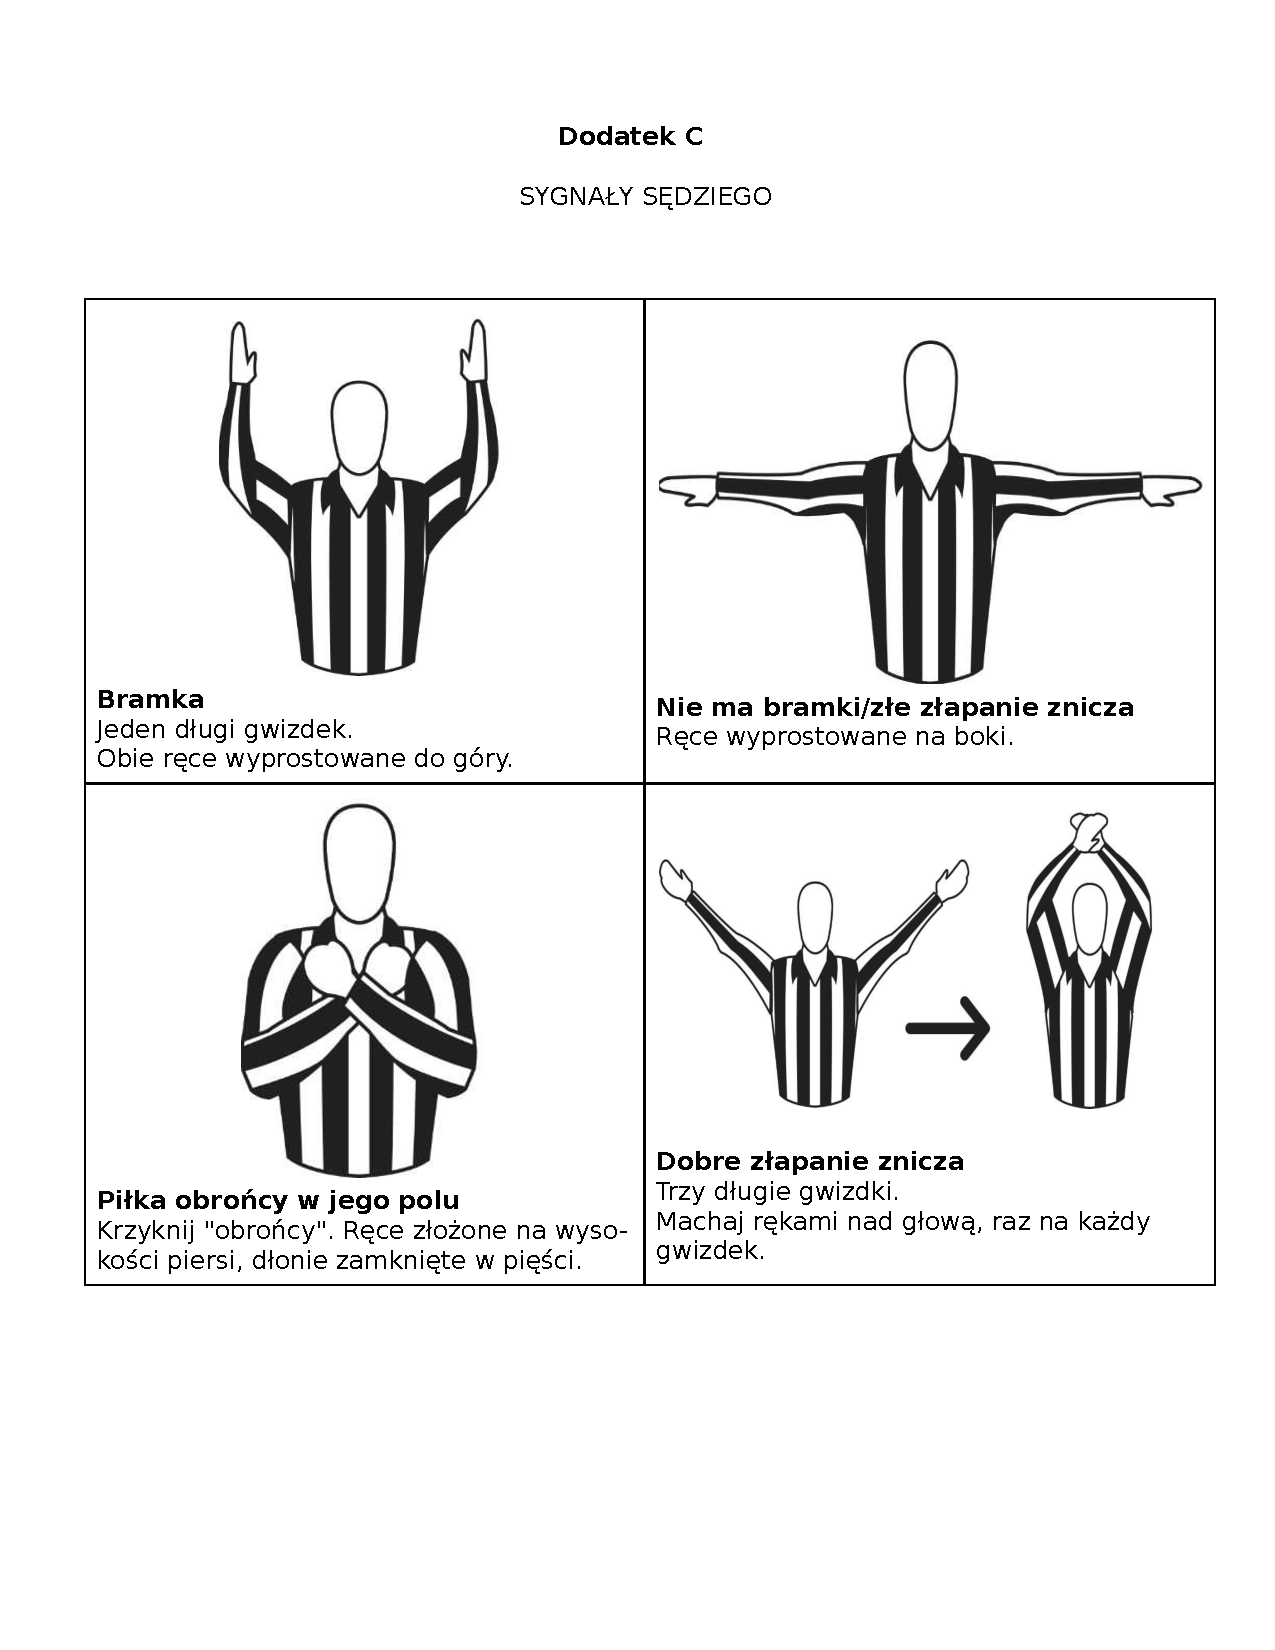
\includepdf[pages={-}]{signals.pdf}

\end{document}
